% !TEX root = ../main.tex

\section{Combinatorial semantics}


\update{Below I will assume that we work with a simple PROP (not coloured)}

Before we begin we first fix some notation.
When $V$ is a set, we denote with $V^{*}$ a set of all finite sequences of the elements of $V$, i.e. $^*$ is a free monoid.
When $\phi : V \to V'$ is a function, we denote with $\phi^{*}$ an extension of $\phi$ to sequences, i.e. $\phi^{*} : V^* \to V'^{*}$ and it applies $\phi$ element-wise.
Similarly, in the case when $\psi \subset V \times V$ is a relation: we denote with $\psi^{*}: \subset V^* \times V^*$ the element-wise relation on ordered sequences.
We will denote with $A +_{f,g} B$ the pushout of $A \xleftarrow{f} C \xrightarrow{g} B$ and will use $i_j$ to denote the $j^{\text{th}}$ injection into a coproduct of the form $X_{j} \xrightarrow{i_{j}} X_{1} + \ldots X_{j} + \ldots X_{n}$ where $+$ denotes the coproduct.

There was a correspondence between hypergraphs and terms in $\textsf{PROP}(\Sigma)$ developed in~\cite{Frobenius, Frobenius2} which we will refer to throughout this section. We first recall the notion of a hypergraph from there.

\Aleksei{Actually, in~\cite{Frobenius} a hypergraph is defined as an object of the corresponding category and labelled hypergraphs are defined as a slice category. This is needed to show adhesiveness. As our category is not adhesive, I think we can follow a more straightforward definition of a tuple.}

\begin{definition}[Category $\catname{Hyp_{\Sigma}}$]


A hypergraph $\mathcal{G}_{\Sigma}$ over a monoidal signature $\Sigma$ is a tuple 
\[
(V_{\mathcal{G}},E_{\mathcal{G}},s,t,l)
\]
\label{def:hypergraph}

where $V_{\mathcal{G}}$ is the set of nodes, $E_{\mathcal{G}}$ is a set of edges, $s : E_{\mathcal{G}} \to V_{\mathcal{G}}^{*}$ is a source function that for each edge returns the ordered list of the edge's source nodes, $t : E_{\mathcal{G}} \to V_{\mathcal{G}}^{*}$ is a target function that for each edge returns the ordered list of the edge's target nodes, $l : E_{\mathcal{G}} \to \Sigma$ is a label function that labels each edge with a generator from monoidal signature $\Sigma$. The label function should satisfy the following conditions: $\forall e,\; \text{s.t.}\; l(e) : m \to n\;. \;|s(e)| = m$ and $\forall e,\; \text{s.t.}\; l(e) : m \to n \;. \;|t(e)| = n$

We will omit the subscripts when they are clear from the context.

A homomorphism $\phi: \mathcal{F} \to \mathcal{G}$ of hypergraphs $\mathcal{F},\mathcal{G}$ is a pair of functions $\phi_V : V_{\mathcal{F}} \to V_{\mathcal{G}}, \phi_E : E_{\mathcal{F}} \to E_{\mathcal{G}}$ such that

\begin{enumerate}
        \item $(s_{\mathcal{F}};\phi_V^*)(e) = (\phi_E;s_{\mathcal{G}})(e)$
    \item $(t_{\mathcal{F}};\phi_V^*)(e) = (\phi_E;t_{\mathcal{G}})(e)$
    \item $l_{\mathcal{F}}(e) = \phi_E;l_{\mathcal{G}}(e)$
\end{enumerate}


Hypergraphs over a monoidal signature $\Sigma$ together with hypergraph homomorphisms form a category $\catname{Hyp_{\Sigma}}$. 
\end{definition}

\begin{definition}[Definition 2.10~\cite{Frobenius}]
Let $\mathbb{C}$ be a category with all finite colimits. A cospan from $X$ to $Y$ is a pair of arrows $X \xrightarrow{} A \xleftarrow{} Y$  in $\mathbb{C}$.

Two cospans $X \xrightarrow{} A \xleftarrow{} Y$ and $X \xrightarrow{} B \xleftarrow{} Y$ are isomorphic if the following diagram commutes and $\alpha$ is iso.

\[
\begin{tikzcd}
                                               & A \arrow[dd, "\alpha"] &                                                \\
X \arrow[ru, bend left] \arrow[rd, bend right] &                        & Y \arrow[ld, bend left] \arrow[lu, bend right] \\
                                               & B                      &                                               
\end{tikzcd}
\]


For $X \in \mathbb{C}$ an $id$-cospan is $X \xrightarrow{id_X} X \xleftarrow{id_X} X$.
The composition of cospans $X \xrightarrow{} A \xleftarrow{f} Y$ and $Y \xrightarrow{g} B \xleftarrow{} Z$ is $X \xrightarrow{} A +_{f,g} B \xleftarrow{} Z$, constructed by taking a pushout of $f,g$.
This data is the category $\catname{Csp(\mathbb{C})}$: the objects are those of $\mathbb{C}$ and the arrows are isomorphism classes of cospans.
Finally, $\catname{Csp(\mathbb{C})}$ is a monoidal category: monoidal product is given by a coproduct (denoted with $+$) in $\mathbb{C}$ and the unit is given by the initial object of $\mathcal{C}$ as can be seen below.

% \[
% \adjustbox{scale=0.75,center}{
% https://q.uiver.app/#q=WzAsMTEsWzAsMCwiQSJdLFsxLDAsIlxcbWF0aGNhbHtHfSJdLFsyLDAsIkIiXSxbMywwLCJcXG90aW1lcyJdLFs0LDAsIkEnIl0sWzYsMCwiQiciXSxbNSwwLCJcXG1hdGhjYWx7Ryd9Il0sWzcsMCwiOj0iXSxbOCwwLCJBK0EnIl0sWzEwLDAsIlxcbWF0aGNhbHtHfStcXG1hdGhjYWx7Ryd9Il0sWzEyLDAsIkIrQiciXSxbMCwxLCJmIl0sWzIsMSwiZyIsMl0sWzQsNiwiZiciXSxbNSw2LCJnJyIsMl0sWzgsOSwiZitmJyJdLFsxMCw5LCJnK2cnIiwyXV0=
% \begin{tikzcd}
% 	A & {\mathcal{G}} & B & \otimes & {A'} & {\mathcal{G'}} & {B'} & {:=} & {A+A'} && {\mathcal{G}+\mathcal{G'}} && {B+B'}
% 	\arrow["f", from=1-1, to=1-2]
% 	\arrow["g"', from=1-3, to=1-2]
% 	\arrow["{f'}", from=1-5, to=1-6]
% 	\arrow["{g'}"', from=1-7, to=1-6]
% 	\arrow["{f+f'}", from=1-9, to=1-11]
% 	\arrow["{g+g'}"', from=1-13, to=1-11]
% \end{tikzcd}
\[
    A \xrightarrow{f} \mathcal{G} \xleftarrow{g} B \otimes A' \xrightarrow{f'} \mathcal{G'} \xleftarrow{g'} B' := A + A' \xrightarrow{f'} \mathcal{G} + \mathcal{G'} \xleftarrow{g'} B + B'
\]

Symmetry is inherited from $\mathcal{C}$ as the coproduct is commutative and is given below.

\[
n + m \xrightarrow{\sigma_{n,m}} m + n \xleftarrow{id + id} m + n
\]

\update{Naturality and SMC laws are implied by $+$ being a coproduct[reference?]}.

\end{definition}


\begin{remark}
    
Taking isomorphism classes of cospans as morphisms turns $\catname{Csp(\mathbb{C})}$ into a proper category since pushouts are defined up to isomorphism and associative.
\end{remark}

When $\mathbb{C} = \catname{Hyp_{\Sigma}}$ we get a category of cospans of hypergraphs.
$\catname{Hyp_{\Sigma}}$ has all finite colimits and, in particular, coproduct is a disjoint union of two hypergraphs.
An empty hypergraph is the initial object in $Hyp_{\Sigma}$ and coproduct and pushout are defined on the underlying sets of nodes and edges.
Following~\cite{Frobenius2} morphisms in an SMC with a signature $\Sigma$ can be interpreted as particular cospans of hypergraphs. 

\begin{definition}[Category $\;\catname{Csp_{D}(Hyp_{\Sigma})}$]
\label{def:cspd}
Category $\catname{Csp_{D}(Hyp_{\Sigma})}$ is a \textit{full} sub-category of $\catname{Csp(Hyp_{\Sigma})}$ which has discrete hypergraphs as objects.
\update{Assuming that $D$ is a functor from PROP to $\catname{Hyp_{\Sigma}}$, $\catname{Csp_{D}(Hyp_{\Sigma})}$ is also a PROP and hence an SMC (Theorem 3.6~\cite{Frobenius}).}
\end{definition}

In particular, this means that any morphism in $\catname{Csp_{D}(Hyp_{\Sigma})}$ is of the form $n \xrightarrow{} \mathcal{G} \xleftarrow{} m$,
where $n,\;m$ are discrete hypergraphs and $\mathcal{G}$ is an arbitrary hypergraph.
When string diagrams are interpreted as cospans of hypergraphs $n,m$ correspond to input and output interfaces of a string diagram respectively.
A pictorial representation of such a cospan is depicted below in Figure~\ref{fig:hypergraph_and_string_diagram}.
We use node labels to define mappings $n \to \mathcal{F}$ and $m \to \mathcal{F}$.

\begin{figure}
    \centering
    \begin{subfigure}{0.45\linewidth}
    \[
    \scalebox{0.6}{
	\tikzfig{combinatorial_semantics/mda-hypergraph-example}
   }
   \]
    \end{subfigure}
    \hfill
    \begin{subfigure}{0.45\linewidth}
        \[
        \raisebox{-0.6cm}{
        \scalebox{0.75}{
        \tikzfig{combinatorial_semantics/mda-hypergraph-example-string}
        }}
        \]
    \end{subfigure}
    \caption{Cospan of hypergraphs and corresponding string diagram}
    \label{fig:hypergraph_and_string_diagram}
\end{figure}

\begin{definition}[Degree of a node] 
The in-degree of a node $v$ in a hypergraph $\mathcal{G}$ is the number of hyperedges $e \in {E_\mathcal{G}}$ such that $v \in s(e)$  Similarly, the out-degree of $v$ is the number of edges $e \in E_\mathcal{G}$ such that $v \in t(e)$.
    
\end{definition}

\begin{definition}[Path]
    A path from $e_0$ to $e_{n-1}$ of length $n$ in a hypergraph $\mathcal{G}$ is an ordered sequence of edges $e_i \in E_{G}$ : $[e_0, e_1, \ldots, e_{n-1}]$ such that for all $i < n - 1$ some node $v \in t(e_i)$ is also in $s(e_{i+1})$.
\end{definition}

\begin{definition}[Acyclicity]
    A hypergraph is acyclic if it contains no paths of length $n > 0$ that start and end in the same edge $e$.
\end{definition}

\begin{definition}[Monogamy]
\label{def:monogamy_hyp}

We call a cospan $n \xrightarrow{f} \mathcal{G} \xleftarrow{g} m$ in $\catname{Csp_{D}(Hyp_{\Sigma})}$ monogamous directed acyclic if

\begin{enumerate}
    \item $\mathcal{G}$ is a directed acyclic hypergraph
    \item $f$ and $g$ are monos
    \item the in-degree and out-degree of every vertex of $\mathcal{G}$ is at most 1
    \item vertices of $\mathcal{G}$ with in-degree 0 are precisely the image of $f$
    \item vertices of $\mathcal{G}$ with out-degree 0 are precisely the image of $g$
\end{enumerate}

\end{definition}

When we narrow our attention to cospans (morphisms) of $\catname{Csp_{D}(Hyp_{\Sigma})}$ which are monogamous we get the category of monogamous directed acyclic (mda-) cospans of hypegraphs $\MdaCospans$.

\begin{definition}[Category $\MdaCospans$]
    We define $\MdaCospans$ as a subcategory of $\catname{Csp_{D}(Hyp_{\Sigma})}$.
\end{definition}

Vertical and horizontal compositions of mda-cospans are mda-cospans, identities and symmetries are mda-cospans, tensor unit is discrete, and hence this is a proper symmetric monoidal category~\cite{Frobenius2}.


\begin{theorem}[Corollary 26~\cite{Frobenius2}]
    $\textsf{PROP}(\Sigma) \cong \MdaCospans$
\end{theorem}
This theorem essentially states a correspondence between morphisms in SMC (string diagrams) and mda-cospans of hypergraphs.

\begin{remark}[Pushout in $\catname{Hyp_{\Sigma}}$]
    Consider a diagram below
    % https://tikzcd.yichuanshen.de/#N4Igdg9gJgpgziAXAbVABwnAlgFyxMJZABgBpiBdUkANwEMAbAVxiRAC0QBfU9TXfIRQBGclVqMWbABrdeIDNjwEiZYePrNWiEAE05fJYKKj11TVJ0AdK3ABmAJzoBjYNIDUursBvYAtgAEAEpcBgr8ykLIAEyk0RqS2iAAitziMFAA5vBEoI4QfkhkIDgQSKISWmx2YfmFiMWlSLGVliCZINQMdABGMAwAChHGOg5YmQAWOLUOBeXUTYgAzOaJbL6OLsBYAPrC3r5YgSEzc4gtiyutSRtOrrvRB7ZHwaE8ebP1F2WIACzUfTAUCQAFolsULEkAFY7aKdEDdPqDYYqUbjKaneoVRb-ECA4HLCFrHQw4SYpBXHGrKo6JhpLhAA

\[
    \adjustbox{scale=1}{
        \begin{tikzcd}
        Z \arrow[r, "f"] \arrow[d, "g"']                                   & X \arrow[d, "\sfrac{i_1}{\sim R}"] \arrow[rdd, "j_1", bend left] &   \\
        Y \arrow[r, "\sfrac{i_2}{\sim R}"] \arrow[rrd, "j_2"', bend right] & \sfrac{X+Y}{\sim R} \arrow[rd, "u"]                              &   \\
                                                                        &                                                                  & Q
        \end{tikzcd}
    }
\]

Pushout of two hypergraphs $X = \{V_{X}, E_{X}, s_{X}, t_{X}\}$ and $Y = \{V_{Y}, E_{Y}, s_{Y}, t_{Y}\}$ (we will omit labelling functions here since they are irrelevant) along $Z$ is computed in two steps.
First, a coproduct of $X$ and $Y$ is taken which is 
\[
    X + Y = \{V_{X} + V_{Y}, E_{X} + E_{Y}, s_{X + Y}, t_{X+Y}\}
\]
where $s_{X+Y} : E_{X} + E_{Y} \to (V_{X} + V_{Y})^{*}$ which can be defined as a copairing $\langle s'_{X}, s'_{Y} \rangle : E_{X} + E_{Y} \to (V_{X} + V_{Y})^{*}$ and $s'_{X} : E_{X} \to (V_{X} + V_{Y})^{*}$, $s'_{Y} : E_{Y} \to (V_{X} + V_{Y})^{*}$ defined as $s'_{X} = s_{X};i_{1,V}^{*}$ and $s'_{Y} = s_{Y};i_{2,V}^{*}$ where $i_1,i_2$ are corresponding coproduct injections, similarly for $t_{X+Y}$.
Recall that each arrow in $\catname{Hyp_{\Sigma}}$ is a pair of arrows for edges and nodes and we will further use subscripts $V$ and $E$ when referring to these functions.
Then, consider relations 
\[
    S_{V} = \{(x_i,y_j) \in (V_{X} + V_{Y}) \times (V_{X} + V_{Y})\; | \; \exists z \in V_{Z} \; . \; x_i = f_{V};i_{1,V}(z) \text{ and } y_j = g_{V};i_{2,V}(z) \text{where $x_i \in V_{X}$ and $y_j \in V_{Y}$ }\}
\]
\[
    S_{E} = \{(x_i,y_j) \in (E_{X} + E_{Y}) \times (E_{X} + E_{Y})\; | \; \exists z \in E_{Z} \; . \; x_i = f_{E};i_{1,E}(z) \text{ and } y_j = g_{E};i_{2,E}(z) \text{where $x_i \in E_{X}$ and $y_j \in E_{Y}$ }\}
\]
and let relations $R_{V}$ and $R_{E}$ be their reflexive symmetric and transitive closures respectively.

\begin{lemma}
    $x R y$ if and only if either $x = y$ or there exists a sequence $(a_1,\ldots,a_{n-1},{a_n})$ such that $x = a_1$ and $y = a_{n}$ such that $a_k S a_{k+1}$ or $a_{k + 1} S a_{k}$ for $k < n$.
\end{lemma}

A quotient of $X+Y$ by these relation is 
\[
    \sfrac{X+Y}{\sim (R_{V},R_{E})} = \{\sfrac{V_{X} + V_{Y}}{\sim R_{V}}, \sfrac{E_{X} + E_{Y}}{\sim R_{E}}, \sfrac{s_{X+Y}}{\sim (R_{V},R_{E})}, \sfrac{t_{X+Y}}{\sim (R_{V},R_{E})}\}
\]
We will then refer to $\sim (R_{V},R_{E})$ just as $\sim$, i.e. writing $\sfrac{V_{X} + V_{Y}}{\sim}$ and the exact relation will be clear from the context.
We have 
\[
    \sfrac{s_{X+Y}}{\sim} : \sfrac{E_{X} + E_{Y}}{\sim} \to (\sfrac{V_{X} + V_{Y}}{\sim})^{*}
\]
In particular, there is an obvious surjective function $[-]_{V} : (V_{X} + V_{Y}) \to (\sfrac{V_{X} + V_{Y}}{\sim})$ that maps elements to their equivalence classes and $[-]_{V}^{*}$ is its extension to sequences. 
Let $s_2 : E_{X} + E_{Y} \to (\sfrac{V_{X} + V_{Y}}{\sim})^{*} = s_{X+Y};[-]^{*}$ and then $\sfrac{s_{X+Y}}{\sim}([e]) = s_{X+Y};[-]^{*}(e) = [s_{X+Y}(e)]^{*}$.
There is also $[-] : E_{X} + E_{Y} \to \sfrac{E_{X} + E_{Y}}{\sim}$ and we will omit subscripts as the correct type will be clear from the argument.
We will also use subscripts when it is important to tell if an element of $E_{X} + E_{Y}$ has in image in either $E_{X}$ or $E_{Y}$ by writing $e_{x}$ or $e_{y}$.
We need to check that if $t_1 \sim t_2$ then $\sfrac{s_{X+Y}}{\sim}([t_1]) = \sfrac{s_{X+Y}}{\sim}([t_2])$. 
There are three options
\begin{enumerate}
    \item $t_1 = e_{y}^{1}$ and $t_2 = e_{y}^{2}$
    \item $t_1 = e_{x}^{1}$ and $t_2 = e_{x}^{2}$
    \item $t_1 = e_{x}$ and $t_2 = e_{y}$ 
\end{enumerate}
We will prove the last point (all the others are analogous).
\begin{proof}
    According to the lemma above $e_{x} \sim e_{y}$ gives us two options.
    \begin{enumerate}
        \item Either $e_{x} = e_{y}$
        \item or there is a sequence $w = (a_1, \ldots, a_{n})$ such that $a_1 = e_{x}$ and $a_{n} = e_{y}$.
    \end{enumerate}
    In the first case the equality holds on the nose.
    We then prove the second case by induction on the length of $w$.
    \begin{itemize}
        \item In the case $|w| = 2$, $e_{x} S e_{y}$ (or $e_{y} S e_{x}$) which means that there exists $z$ in $E_{Z}$ such that $f_{E};i_{1,E}(z) = e_{x}$ and $g_{E};i_{2,E}(z) = e_{y}$.
              Recall that because $f$ and $g$ are homomorphisms, the following equalities hold
              \[
                s_{Z};f_{V}^{*};i_{1,V}^{*}(z) = f_{E};i_{1,E};s_{X+Y}(z) = s_{X+Y}(e_{x})
              \]
              \[
                s_{Z};g_{V}^{*};i_{2,V}^{*}(z) = g_{E};i_{2,E};s_{X+Y}(z) = s_{X+Y}(e_{y})
              \]
              Then,
              \[
                \sfrac{s_{X+Y}}{\sim}([e_{x}]) = [s_{X+Y}(e_{x})]^{*} = [s_{Z};f_{V}^{*};i_{1,V}^{*}(z)]^{*}
              \]
              and
              \[
                \sfrac{s_{X+Y}}{\sim}([e_{y}]) = [s_{X+Y}(e_{y})]^{*} = [s_{Z};g_{V}^{*};i_{2,V}^{*}(z)]^{*}
              \]
              Then, by noting that $f_{V};i_{1,V}(z) = g_{V};i_{2,V}(z)$ for all $z$ in $V_{Z}$ (because $\sfrac{V_{X} + V_{Y}}{\sim}$ is so defined) we have $[s_{X+Y};(e_{x})]^{*} = [s_{X+Y}(e_{y})]^{*}$.
        \item Suppose if $e_{x} S e_{y}$ by a chain of length $n$ or less then $[s_{X+Y}(e_{x})]^{*} = [s_{X+Y}(e_{y})]^{*}$.
        \item Now suppose $e_{x} S e_{y}$ by a chain $w = (a_1, \ldots, a_{n+1})$ and a subchain $(a_1, \ldots, a_{n})$ satisfies the inductive hypothesis and hence $s_{X+Y};s_{1}^{*}(e_{x}) = s_{X+Y};s_{1}^{*}(a_{n})$.
              Note that $S_{E}, S_{V}$ relate only elements with the pre-image in $E_{X}$ (respectively, $V_{X}$) with elements with the pre-image in $E_{Y}$ (respectively, $V_{Y}$). 
              Elements with the pre-image in the same set are not related.
              Then we have $a_n S a_{n+1} = e_{y}$ and need to show that $[s_{X+Y}(a_{n+1})]^{*} = [s_{X+Y}(e_{y})]^{*}$.
              This follows by exactly the same argument as the base case as $a_{n+1}$ is necessarily in $E_{X}$.
              And we finally have $[s_{X+Y}(e_{x})]^{*} = [s_{X+Y}(a_{n+1})]^{*} = [s_{X+Y}(e_{y})]^{*}$.
    \end{itemize}
    \update{Looks fine?}
\end{proof}

Next 
\[
    \sfrac{i_{1,V}}{\sim} : V_{X} \to \sfrac{V_{X} + V_{Y}}{\sim} = [i_{1,V}]
\]
and
\[
\sfrac{i_{1,E}}{\sim} : E_{X} \to \sfrac{E_{X} + E_{Y}}{\sim} = [i_{1,E}]
\]
similarly for $\sfrac{i_{2,E}}{\sim}$ and $\sfrac{i_{2,V}}{\sim}$
We need to show
\begin{enumerate}
    \item $s_{X};(\sfrac{i_{1,V}}{\sim})^{*}(e) = \sfrac{i_{1,E}}{\sim};\sfrac{s_{X+Y}}{\sim}(e)$
    \item $t_{X};(\sfrac{i_{1,V}}{\sim})^{*}(e) = \sfrac{i_{1,E}}{\sim};\sfrac{t_{X+Y}}{\sim}(e)$
\end{enumerate}
and likewise for $i_{2}$.
Let's check the first one for which we first need to check that $([-]_{E},[-]_{V})$ is a homomorphisms, i.e.
\[
[s_{X+Y}(e)]^{*} = \sfrac{s_{X+Y}}{\sim}([e]) = [s_{X+Y}(e)]^{*}
\]
hence, $(\sfrac{i_{1,V}}{\sim}, \sfrac{i_{1,E}}{\sim})$ is a homomorphism because $(i_{1,V},i_{1,E})$ and $([-]_{E},[-]_{V})$ are.

% Note that if $s : e_1 \mapsto \{v_1,v_2\}$ and $s : e_2 \mapsto \{v_3,v_4\}$  and $e_1 \sim e_2$ then $\sfrac{s}{\sim R} : [e_1,e_2] \to \{[v_1,v_3],[v_2,v_4]\}$ because $f$ and $g$ are homomorphisms.
% Then, $\sfrac{i_1}{\sim R}$ maps $y \in Y$ to its equivalence class and likewise for $\sfrac{i_2}{\sim R}$.
% we will denote the equivalence classes in $\sfrac{X + Y}{\sim R}$ as $[x]$ and $[y]$ depending on their pre-image being either in $X$ or $Y$.
% Before we procced, we need to show that $\sfrac{i_1}{\sim R}$ and $\sfrac{i_2}{\sim R}$ are homomorphisms.
% Let $e_{x}$ be an edge in $X$ and $v_x$ is its source. We need to check that $\sfrac{i_1}{\sim R}(v_x) = (\sfrac{i_1}{\sim R};\sfrac{s_{X}}{\sim R})(e_x)$.
% $\sfrac{i_1}{\sim R}(v_x) = [v_x]$ and $(\sfrac{i_1}{\sim R};\sfrac{s_{X}}{\sim R})(e_x) = \sfrac{s_{X}}{\sim R}([e_x]) = [v_x]$ and hence $\sfrac{i_1}{\sim R}$ is a homomorphism, simialrly $\sfrac{i_2}{\sim R}$ is.
Now, the square obviously commutes.
To show that $\sfrac{X + Y}{\sim}$ is a pushout we need to argue that for each $Q$ and morphisms $j_1 = (j_{1,V}, j_{1,E})$ and $j_2 = (j_{2,V}, j_{2,E})$ such that the above square commutes there is a unique $u = (u_{V}, u_{E})$ such that $j_1 = \sfrac{i_{1}}{\sim} ; u$ and $j_2 = \sfrac{i_2}{\sim} ; u$.
We will define such $u$ as $u_{E}([i_{1,E}(e_{x})]) = j_{1,E}(e_{x})$ and $u_{E}([i_{2,E}(e_{y})]) = j_{2,E}(e_y)$ (similarly for $u_{V}$) and claim that it is a well-defined function by showing that if $t_1 \sim t_2$ then $u_{E}(t_1) = u_{E}(t_2)$.
There are three options analogoues to the proof above, so we will show the base case for $t_1 = i_{1,E}(e_{x})$ and $t_2 = i_{2,E}(e_{y})$.
$t_1 \sim t_2$ implies that there exists at least one $z$ in $E_{Z}$ such that $i_{1,E}(e_{x}) = f_{E};i_{1,E}(z)$ (or $e_{x} = f_{E}(z)$) and $[i_{1,E}(e_{x})] = \sfrac{i_{1,V}}{\sim}(e_x)$, and $e_y = g_{E}(z)$ $[in_{2,E}(e_{y})] = \sfrac{i_{2,V}}{\sim}(e_y)$.
By applying $j_{1,E}$ to the first we get $j_{1,E}(f_{E}(z)) = j_{1,E}(e_x)$ and similarly for $j_{2,E}$: $j_{2,E}(g_{E}(z)) = j_{2,E}(e_y)$ and $j_{1,E}(e_{x}) = j_{2,E}(e_{y})$ by commutativity.
Hence, $u_{E}([in_{1,E}(e_x)]) = u_{E}([in_{2,E}(e_y)])$.
\update{Above $e_x$ and $e_y$ are different from $e_x$ and $e_y$ from the first proof, i.e. they are in $E_{X}$ and $E_{Y}$. This is probablty not good.}

\question{Next, $u$ is a homomorphism because $j_1$ and $j_2$ are.}
Finally, $u$ is unique.
Assume, that there exists $w : \sfrac{X+Y}{\sim R} \to Q$ for the same $j_1$ and $j_2$.
In order for them to commute $w_{E}([i_{1,E}(x)]) = j_1(x)$ and $w([in_{2,E}(y)]) = j_2(y)$ (similarly for $w_{V}$) which is the same as $u_{E}$.
That is, $j_1$ and $j_2$ determine $u$ uniquely.

\end{remark}

Now we are ready to define e-hypergraphs which are a combinatorial representation of enriched PROPs.

\begin{definition}[E-hypergraph]

    An e-hypergraph $\mathcal{G}$ over a monoidal signature $\Sigma$ is a tuple \[(V_{\mathcal{G}},E_{\mathcal{G}},s,t,l,<_c,\#)\] where $(V_{\mathcal{G}},E_{\mathcal{G}},s,t)$ are the same as in~\ref{def:hypergraph}.
    The labelling $l$ is modified to include an extra value $\bot \;$ $l :E_{\mathcal{G}} \to \Sigma + 1$. 
    % With an abuse of notation, we will confuse $\mathcal{G}$ with $V_{\mathcal{G}} \cup E_{\mathcal{G}}$, when treating it as a set.
    \question{Shall I use $\cup$ instead of $+$?}
    $<_c \subset (V_\mathcal{G} + E_\mathcal{G}) \times (V_\mathcal{G} + E_\mathcal{G})$ is a child relation imposing a strict partial order on $(V_\mathcal{G} + E_\mathcal{G})$.
    We require that for a given $x \in (V_\mathcal{G} + E_\mathcal{G})$ a set of all predecessors of $x\;$ $[x) = \{x' \in E_\mathcal{G} \;||\; x' <_c x\; \}$ is finite and consists of edges $e \in E_{\mathcal{G}}$ such that $l(e) = \bot$ only.
    Next, each $x$ has at most one immediate predecessor.
    \update{We will denote the fact that $e$ is an immediate predecessor of $v$ as $e <_c^{\mu} v$.}
    Similarly, a set of all successors is $(x] = \{x' \in (V_\mathcal{G} + E_\mathcal{G}) \; ||\; x <_{c} x'\}$ where $x'$ can be a node or an edge. 
    % An edge $e \in E_{\mathcal{G}}$ is unlabelled, i.e. $l(e) = \bot$ iff $(e] \not = \varnothing$.
    Finally, we require that $<_c^{\mu}$ respects connectivity, i.e. if $v \in s(e)$ then $e' <_c^{\mu} e$ iff $e' <_c^{\mu} v$.

    Then, consider a relation $\consistency^{\mu} \subseteq (V_{\mathcal{G}} + E_{\mathcal{G}}) \times (V_{\mathcal{G}} + E_{\mathcal{G}})$ which we will call a \textit{consistency} relation and which has the following properties.
    \begin{enumerate}
        \label{def:consistency_properties}
        \item The relation is an equivalence relation
        \item If $v \in s(e)$ then $v \consistency^{\mu} e$
        \item If $v \in t(e)$ then $v \consistency^{\mu} e$
        \item The relation is defined only for edges $e$ and nodes $v$ such that $[v) = [e) \not = \varnothing$
    \end{enumerate}
    
%     $\langle (V_\mathcal{G} + E_\mathcal{G}), <_c, \# \rangle$ is an event-structure where $\# \subset (V_\mathcal{G} + E_\mathcal{G}) \times (V_\mathcal{G} + E_\mathcal{G})$ is an irreflexive symmetric relation called \textit{conflict} relation which satisfies the following
%     \begin{enumerate}
%         \label{def:e-hypergraph-req}
%         \item 
%         \[
%     \forall x_1, x_2, x_3 \in (V_\mathcal{G} + E_\mathcal{G}) \text{, if } x_1 <_c x_2 \text{ and } x_1 \# x_3 \text{ then } x_2 \# x_3
%     \] 
%     if $x_1 <_c x_2$ we say that conflict $x_2 \# x_3$ is inherited from the conflict $x_1 \# x_3$. If the conflict is not inherited we say it is \textit{immediate} and denote it with $\#_{\mu}$
%     \item $<_c$ and $\#$ are mutually exclusive
%     \item $\#$ is defined \textit{only} for $x \in (V_\mathcal{G} + E_\mathcal{G})$ such that $[x) \not \eq \varnothing$
%     \item $\#$ should respect connectivity
%     \item \update{Complement of $\hashtag_{\mu}$ should be transitive}
%     \item for all distinct $x_1, x_2, x_3 \in (V_\mathcal{G} + E_\mathcal{G})$ $x_1 \#_{\mu} x_2$ and $x_2 \#_{\mu} x_3$ implies $x_1 \#_{\mu} x_3$
%     \item for all $x, x' \in (V_\mathcal{G} + E_\mathcal{G})$ $x \#_{\mu} x'$ implies $[x) = [x')$
%         \end{enumerate}

% The last two requirements are known as \textit{confusion freeness}~\cite{ConfusionFreeEvents}.
\end{definition}

% Intuitively, the child and conflict relation together make it possible to model e-classes in our e-hypergraphs: an unlabelled edge $e$ represents an e-class where the children of $e$ that are in immediate conflict correspond to nodes and edges in different e-class instances.
% Condition (5) states that the following situation is not possible: $x_1 \# x_3$ and $x_1 \bar{\#} x_2$ and $x_2 \bar{\#} x_3$.
% Transitivity of $\bar{\#}$ requires that in this case $x_1 \bar{\#} x_3$.

% \begin{lemma}[Complement of $\#$ is equivalence relation]
% \begin{proof}
% As $\#$ is irreflexive then its complement $\bar{\#}$ is reflexive because $\forall x \; . \; (x,x) \not \in \#$. Because $\#$ is symmetric so is $\bar{\#}$, otherwise if $(x_1, x_2) \in \bar{\#}$ and $(x_2,x_1) \not \in \bar{\#}$ then $(x_2,x_1) \in {\#}$ which is symmetric and hence $(x_1,x_2)$ should be in ${\#}$.
% Finally, the complement is transitive because of (5).

% \end{proof}
% \end{lemma}


\begin{remark}
    We will further call edges $e$ such that $l(e) = \bot$ \textit{hierarchical}.
    We will also refer to edges $e$ and nodes $v$ such that $[e) = \varnothing$ and $[v) = \varnothing$ as top-level.
\end{remark}

\begin{remark}
    Because $\consistency^{\mu}$ respects connectivity and is reflexive, symmetric and transitive, it is essentially a relation between connected components that have the same predecessor.
    This notion will be helpful in the following example.
\end{remark}
% We associate an e-class with a hierarchical edge, i.e. an edge with children. 
% The parent functions satisfy some conditions. First, an edge and any of its source and target vertices must have the same parent: $p_V (v) = p_E(e) = p_V (v')$ for all $v \in s(e)$ and $v' \in t(e)$, respectively.
% Second, the parent relation must be acyclic.
% More precisely, we assume for all $e \in E$ there is some $k \geq 1$ such that $(p_E,\bot)k(e) = \bot$ where $\bot$ is the element of $1$ and $p_{E,\bot} :E+1 \to E+1$ is the extension of $p_E$ adding $p_{E,\bot}(\bot)=\bot$.


% $\#_{V}$ and $\#_{E}$ are conflict relations that tell whether nodes and edges belong to different instances within an e-class: if the elements are in conflict, they belong to different instances. \update{E-classes are represented by edges $e : l_E(e) = \bot$. Hence, the conflict relation $\#_{V}$ between $v_1$ and $v_2$ is defined only when $p_V(e_1) \not \eq \bot$ and $p_V(e_2) \not \eq \bot$. Likewise the conflict relation $\#_{E}$ between $e_1$ and $e_2$ is defined only when $p_{E}(e_1) \not \eq \bot$ and $p_{E}(e_2) \not \eq \bot$}



% The relation should respect connectivity, that is, if $e_1 \#_E e_2$ then $s(e_1) \#_V^* s(e_2)$ and $t(e_1) \#_V^* t(e_2)$, where $\#_V^*$ is element-wise relation. 
% % This guarantees that related nodes and edges are contained within the same e-class.
% \update{
% We also require that if $v_1 \#_{V} v_2$ then $\forall e_1,e_2 : v_1 \in s(e_1)$ and $v_2 \in s(e_2)\; e_1 \#_{E} e_2$  and the same for the case when $v_i \in t(e_1),\;v_j \in t(e_2)$. Finally, the relation should be \textit{hereditary}: if $e_1 \#_E e_2 \text{ and } \forall n,m,k,q > 0, \; v_1,v_2 \in V_{\mathcal{G}} \text{ and } e_1', e_2' \in E_{\mathcal{G}} \text{ s.t. } p^n(v_1) = e_1, \; p^m(v_2) = e_2, \; p^k(e_1') = e_1, \; p^q(e_2') = e_2\; . \;
%  v_1 \#_V v_2 \text{ and } e_1' \#_E e_2'$. Where $p^n(v),\; n > 0$ is $n^{th}$ parent of $v$} The relation is also irreflexive and symmetric.

\begin{example}
    
A few examples of e-hypergraphs (and their corresponding graphical interpretation) can be seen in Figure~\ref{fig:e-hypergraph-example}.
In example~\ref{fig:example_a} the relations $<_{c}$ and $\consistency^{\mu}$ are the following
\[
    <_{c} = \{(v_3,e_1), (e_2, e_1), (v_4, e_1) \}
\] and 
\begin{align*}
    \consistency^{\mu} = \{ (v_1,e_1),
                            (v_2, e_1), 
                            (v_3,e_2), (v_4,e_2)\}^{c}
\end{align*}
where $c$ denotes the reflexive, syymetric and transitive closure.
In other words, $e_1$ is the predecessor of the connected component that contains edge $e_2$ and this connected component is consistent with itself only.
The connected component that contains $e_1$ is also consistent with itself only.

In the next example~\ref{fig:example_b} $e_1$ is the predecessor of two connected components but these components are consistent only with themselves.
We denote this fact by using a vertical line. 
Practically, hierarchical edges such as $e_1$ represent e-classes and connected components which are pairwise not consistent belong to different instances of the same e-class.

In the last example~\ref{fig:example_c} two connected components that contain $e_2$ and $e_3$ respectively are consistent with themselves and with each other.
\end{example}

\begin{figure}[t]
    \begin{subfigure}{0.3\linewidth}
        \[
            \scalebox{0.6}{
                \tikzfig{combinatorial_semantics/e-hypergraph-example-1}
            }
            \]
        \caption{}
        \label{fig:example_a}
    \end{subfigure}
    \hfill
    \begin{subfigure}{0.3\linewidth}
        \[
          \scalebox{0.6}{
            \tikzfig{combinatorial_semantics/e-hypergraph-example-2}
          }  
        \]
        \caption{}
        \label{fig:example_b}
    \end{subfigure}
    \hfill
    \begin{subfigure}{0.3\linewidth}
        \[
          \scalebox{0.6}{
            \tikzfig{combinatorial_semantics/e-hypergraph-example-3}
          }  
        \]
        \caption{}
        \label{fig:example_c}
    \end{subfigure}
    \caption{E-hypergraph examples}
    \label{fig:e-hypergraph-example}
\end{figure}

\begin{example}
An example of an e-hypergraph can be found in Figure~\ref{fig:e-cospan}.
The e-hypergraph is depicted in the area shaded grey.
Edges $g$ and $h$ are in conflict (as well as their incoming and outcoming nodes) and they share the same predecessor --- the edge shaded with lighter colour. 
Vertical line delimits the edges and nodes which are in conflict. 
Intuitively, such lines delimit e-class instances.
\end{example}

\begin{definition}[Convex subgraph]
  We call a subgraph $\mathcal{H}$ of an e-hypergraph $\mathcal{G}$ convex if for all $v_i, v_j \in V_{\mathcal{H}}$ all $v_k \in path(v_i, v_j)$ are also in $\mathcal{H}$.
\end{definition}


\begin{definition}[Down-closed subgraph]
    We call a subgraph $\mathcal{H}$ of an e-hypergraph $\mathcal{G}$ down-closed if for all $e \in E_{\mathcal{H}}$ all elements of $(e]$ are also in $\mathcal{H}$.
\end{definition}

 % \begin{remark}
 %    We will use $p_{E}^n(e)$ as a syntactic sugar for $p_{E,\bot} ; p_{E,\bot} \ldots p_{E,\bot}(e)$ to denote the n$^{th}$ parent of an edge $e$. Similarly
 %     we will use $p_{V}^n(v)$ as a syntactic sugar for $p_{E}^{n-1};p_{V}(v)$ to denote the n$^{th}$ parent of a node $v$.
 % \end{remark}

\begin{remark}
    Both relations can be considered as functions defined on $V_{\mathcal{F}} + E_{\mathcal{F}}$, i.e. on the coproduct of nodes and edges.
    To make things well-typed, we will use corresponding coproduct injections $i_{V_{\mathcal{F}}} \to V_{\mathcal{F}} + E_{\mathcal{F}}$ and $i_{E_{\mathcal{F}}} \to V_{\mathcal{F}} + E_{\mathcal{F}}$ when passing either node or edge into these functions.
    For example, an immediate successor of a node $x$ can be written functionally as $<_{c,\mathcal{F}}^{\mu}(i_{V_{\mathcal{F}}}(x))$.
\end{remark}

\begin{definition}{E-hypergraphs homomorphism}
\label{def:e-homo}    
A homomorphism $\phi: \mathcal{F} \to \mathcal{G}$ of e-hypergraphs $\mathcal{F},\mathcal{G}$ is a pair of functions $\phi_V : V_{\mathcal{F}} \to V_{\mathcal{G}}, \phi_E : E_{\mathcal{F}} \to E_{\mathcal{G}}$ such that

\begin{enumerate}
    \item $\phi$ is hypergraph homomorphism
    
    \item \[
        \phi_{E}(<_{c,\mathcal{F}}^{\mu}(i_{V_{\mathcal{F}}}(x))) = <_{c,\mathcal{G}}^{\mu}(\phi_{V};i_{V_{\mathcal{G}}}(x))
        \] when $x$ is a node,
        and
        \[
        \phi_{E}(<_{c,\mathcal{F}}^{\mu}(i_{E_{\mathcal{F}}}(x))) = <_{c,\mathcal{G}}^{\mu}(\phi_{E};i_{E_{\mathcal{G}}}(x))  
        \] when $x$ is an edge.
          \update{We do not require such an equation when $[x) = \varnothing$}.

    % \item
    % $x_1 \#_{\mathcal{F}} x_2$ iff $\phi(x_1) \#_{\mathcal{G}} \phi(x_2)$, where $x_1, x_2 \in \mathcal{F}$
  
        \item
    if $x_1 \consistency_{\mathcal{F}}^{\mu} x_2$ then $\phi(x_1) \consistency_{\mathcal{G}}^{\mu} \phi(x_2)$, where $x_1, x_2 \in \mathcal{F}$.
    Or, written functionally, when $x \in E_{\mathcal{F}}$
    \[
        \langle \phi_{V};i_{V_{\mathcal{G}}}, \phi_{E};i_{E_{\mathcal{G}}} \rangle^{*}(\consistency_{\mathcal{F}}^{\mu}(i_{E_{\mathcal{F}}}(x)))
        \subseteq
        \consistency_{\mathcal{G}}^{\mu}(\phi_{E};i_{E_{\mathcal{G}}}(x))
    \]
    , where $\phi_{V};i_{V_{\mathcal{G}}} : V_{\mathcal{F}} \to V_{\mathcal{G}} + E_{\mathcal{G}}$, and similarly for $\phi_{E};i_{E_\mathcal{G}}$ so that $\langle \phi_{V};i_{V_{\mathcal{G}}}, \phi_{E};i_{E_{\mathcal{G}}} \rangle : V_{\mathcal{F}} + E_{\mathcal{F}} \to  V_{\mathcal{G}} + E_{\mathcal{G}}$.
    And, when $x \in V_{\mathcal{F}}$
    \[
        \langle \phi_{V};i_{V_{\mathcal{G}}}, \phi_{E};i_{E_{\mathcal{G}}} \rangle^{*}(\consistency_{\mathcal{F}}^{\mu}(i_{V_{\mathcal{F}}}(x)))
        \subseteq
        \consistency_{\mathcal{G}}^{\mu}(\phi_{V};i_{V_{\mathcal{G}}}(x))
    \]
    % Or, on per-component basis, if $i_{E_{\mathcal{F}}}(x_1) \in \hashtag_{\mathcal{F}}(i_{E_{\mathcal{F}}}(x_2))$ then $i_{E_{\mathcal{G}}}(\phi_{E}(x_1)) \in \hashtag_{\mathcal{G}}(i_{E_{\mathcal{G}}}(\phi_{E}(x_2)))$ and similarly for other types of $x_1,x_2$.
\end{enumerate}

% \update{Let's denote the fact of $x_1$ being the immediate predecessor of $x_2$ by $x_1 <_{\mu} x_2$.
%  Also, note that preserving the immediate predecessor implies preserving order.
% Homomorphism definition seems to be fine: by not requiring the \textit{only if} direction in bullet 2 we basically allow either of two things 

% \begin{itemize}
%     \item $\phi(x_1) <_{\mu} \phi(x_2)$ and $x_1 <_{\mu} x_2$
%     \item $\phi(x_1) <_{\mu} \phi(x_2)$ and $x_1$ is unrelated to $x_2$
% \end{itemize}

% We can not have $\phi(x_1) <_{\mu} \phi(x_2)$ and $x_1 < x_2$, i.e. the case where $x_1$ is not the immediate predecessor of $x_2$ because then it would mean that there exists at least $x_3$ such that $x_1 <_{\mu} x_3 <_{\mu} x_2$ and because $\phi$ should preserve them it would mean that $\phi(x_1) <_{\mu} \phi(x_3) <_{\mu} \phi(x_2)$ implying that $\phi(x_2)$ has two immediate predecessors: $\phi(x_1)$ and $\phi(x_3)$.
% Of course, if $\phi$ does not identify $x_1$ and $x_3$.
% The first bullet is fine because it means that $\phi$ reflects the immediate predecessor.
% The second bullet leaves us with two options depicted above.

% }

% \begin{figure}
%     \centering
% \begin{subfigure}{0.4\linewidth}

% \scalebox{0.5}{
% \begin{tikzpicture}
% 	\begin{pgfonlayer}{nodelayer}
% 		\node [style=node, label={above:$x_1$}] (19) at (-3.5, -4.5) {};
% 		\node [style=node, label={above:$x_2$}] (20) at (-4.5, -6.5) {};
% 		\node [style=node, label={above:$x_3$}] (21) at (-2.5, -6.5) {};
% 		\node [style=node, label={above:$x_4$}] (22) at (-3.5, -8.5) {};
% 		\node [style=node, label={above:$x_5$}] (23) at (-1.5, -8.5) {};
% 		\node [style=node, label={right:$x_2$}] (24) at (4.5, -5.5) {};
% 		\node [style=node, label={above:$x_1$}] (25) at (4.5, -2.5) {};
% 		\node [style=node, label={below:$x_5$}] (26) at (4.5, -11.5) {};
% 		\node [style=none] (27) at (4.5, -7.5) {};
% 		\node [style=none] (28) at (4.5, -9.5) {};
% 		\node [style=none] (29) at (4.5, -8.5) {$\vdots$};
% 		\node [style=none] (30) at (0.5, -6.5) {};
% 		\node [style=none] (31) at (2.5, -6.5) {};
% 		\node [style=none] (32) at (1.5, -5.5) {$\phi$};
% 	\end{pgfonlayer}
% 	\begin{pgfonlayer}{edgelayer}
% 		\draw (19) to (20);
% 		\draw (19) to (21);
% 		\draw (21) to (22);
% 		\draw (21) to (23);
% 		\draw (24) to (27.center);
% 		\draw (26) to (28.center);
% 		\draw (25) to (24);
% 		\draw [style=diredge] (30.center) to (31.center);
% 	\end{pgfonlayer}
% \end{tikzpicture}

% }

% \caption{Case 1}
% \end{subfigure}
% \hfill
% \begin{subfigure}{0.4\linewidth}

% \scalebox{0.5}{
% \begin{tikzpicture}
% 	\begin{pgfonlayer}{nodelayer}
% 		\node [style=node, label={above:$x_1$}] (19) at (-6.5, -4.5) {};
% 		\node [style=node, label={above:$x_2$}] (20) at (-7.5, -6.5) {};
% 		\node [style=node, label={above:$x_3$}] (21) at (-5.5, -6.5) {};
% 		\node [style=node, label={above:$x_4$}] (30) at (-3, -4.5) {};
% 		\node [style=node, label={above:$x_1$}] (31) at (2.5, -4.5) {};
% 		\node [style=node, label={above:$x_2$}] (32) at (1.5, -6.5) {};
% 		\node [style=node, label={above:$x_3$}] (33) at (2.75, -6.5) {};
% 		\node [style=node, label={above:$x_4$}] (34) at (4, -6.5) {};
% 		\node [style=none] (35) at (-1.5, -5.5) {};
% 		\node [style=none] (36) at (-0.5, -5.5) {};
% 		\node [style=none] (37) at (-1, -5) {$\phi$};
% 	\end{pgfonlayer}
% 	\begin{pgfonlayer}{edgelayer}
% 		\draw (19) to (20);
% 		\draw (19) to (21);
% 		\draw (31) to (32);
% 		\draw (31) to (33);
% 		\draw (31) to (34);
% 		\draw [style=diredge] (35.center) to (36.center);
% 	\end{pgfonlayer}
% \end{tikzpicture}

% }

% \caption{Case 2}
    
% \end{subfigure}
% \end{figure}

% \update{Case (a) above is impossible on two occasions: for the image of $x_5$ to be a successor of the image of $x_2$, $x_5$ itself should be hierarchical. Then, because $\phi$ should preserve the immediate predecessor, the image of $x_3$ should be the immediate predecessor of the image of $x_5$ and the image of $x_1$ should be the immediate predecessor of the image of $x_3$ and of the image of $x_2$. Since the image of $x_2$ is a successor of the image of $x_5$ on the right there should be two paths from the image of $x_5$ to the image of $x_1$ one through the image of $x_3$ and another through the image of $x_2$, this effectively means that some node on this path has two immediate predecessors.

% The case (b) above typechecks (for typed e-hypergraphs) only if $x_4$ is of type $0 \to 0$. This case is fine because we always can append, e.g. an edge, to a hierarchical edge using the semilattice equations (the one for tensoring the box). This also assumes that the image is down-closed.
% }

% \question{There is an issue with requiring that $\phi$ should reflect the conflict though. When we consider e-cospans and the maps from the interfaces to the carrier we map some nodes from the interface to conflicted nodes in the carrier. However, these nodes in the interface can not be in conflict as they have no predecessors. We can ask that this is a property of a matching morphism $m$ rather than arbitrary homomorphism. The same was done for down-closed-ness, for example.
% }

If we further require that if $[x_1) = \varnothing$ then $[\phi(x_1)) = \varnothing$ we will call such homomorphism \textit{strict}.
\end{definition}


% The last 2 conditions say that if two elements are from different instances of an e-class, then, under a homomorphism they shall remain in different instances. that is, homomorphism should preserve and reflect conflicts.

% \question{If we do not introduce $\bot$ as a parent, we do not need a notion of a weaker homomorphism. That is point 2 above suffices. Is is enough or shall we require the preservation of the immediate predecessor?}

In other words, homomorphism should preserve immediate predecessors and the conflict relation.

\begin{remark}
    When we consider an image of $\mathcal{F}$ under $\phi$ in $\mathcal{G}$ as an e-hypergraph in its own rights we assign $[x) = \varnothing$ for all $x$ whose immediate predecessor $x'$ not in the image of $\phi$.
\end{remark}

\begin{definition}[Category $\catname{EHyp_{\Sigma}}$]
Such e-hypergraphs form a category $\catname{EHyp_{\Sigma}}$ where morphisms are e-hypergraph homomorphisms defined above.
In particular, it has a coproduct which is a disjoint union of e-hypergraphs and a tensor unit which is an empty e-hypergraphs with empty relations which makes it into a monoidal category.
\end{definition}

\begin{definition}[Pushout in $\catname{EHyp_{\Sigma}}$]

    We will compute pushouts in $\catname{EHyp_{\Sigma}}$ similarly to $\catname{Hyp_{\Sigma}}$ but additionally will make a few assumptions.
    Recall the diagram below.
    \[
    \adjustbox{scale=1}{
        \begin{tikzcd}
        Z \arrow[r, "f"] \arrow[d, "g"']                                   & X \arrow[d, "\sfrac{i_1}{\sim R}"] \arrow[rdd, "j_1", bend left] &   \\
        Y \arrow[r, "\sfrac{i_2}{\sim R}"] \arrow[rrd, "j_2"', bend right] & \sfrac{X+Y}{\sim R} \arrow[rd, "u"]                              &   \\
                                                                        &                                                                  & Q
        \end{tikzcd}
    }
    \]

    \begin{enumerate}
    \item $Z$ is a \textit{discrete} e-hypergraph, i.e. it has no edges.
    \item $[f_{V}(v_i)) = [f_{V}(v_j))$ and $[g_{V}(v_i)) = [g_{V}(v_j))$ for all $v_i,v_j \in V_{Z}$. \update{This essentially means that $f,g$ do not map nodes to levels of different hierarchy.}
    \item If $[f_{V}(v)) \not = \varnothing$ then $[g_{V}(v)) = \varnothing$ and vice versa.
    \item $\consistency^{\mu}(f(v_i)) = \consistency^{\mu}(f(v_j))$ and $\consistency^{\mu}(f(g_i)) = \consistency^{\mu}(g(v_j))$.
    \item $f$ and $g$ are mono.
    \label{pushout:assumptions}
    \end{enumerate}

    Then, the pushout of e-hypergraphs $X$ and $Y$ is computed in two steps.
    First, a coproduct of $X+Y$ is computed which is 
    \[
        X + Y = \{V_{X} + V_{Y}, E_{X} + E_{Y}, s_{X+Y}, t_{X+Y}, \consistency_{X+Y}, <_{c,X+Y} \}
    \]
    
    once again omitting the labelling function and where source and target functions are as before.
    And consider the same relations $S_{V},S_{E}$ and $R_{V}, R_{E}$.

    % \update{Now $<_{c,{X+Y}} : V_{X} + V_{Y} + E_{X} + E_{Y} \to E_{X} + E_{Y} + \bot_{X} + \bot_{Y}$
    % And let's get back to the case when $<_{c,Z}^{\mu}(z) = \bot_{Z}$, $<_{c,X}^{\mu}(f_{V}(z)) = \bot_{X}$, $f_{E}(\bot_{Z}) = \bot_{X}$ and $g_{E}(\bot_{Z}) = <_{c,Y}^{\mu}(g_{V}(z))$
    % We then want to show that $[<_{c,X+Y}^{\mu}(f_{V};i_{1,V}(z))] = [<_{c,X+Y}^{\mu}(g_{V};i_{2,V}(z))]$
    % Note that we have $[i_{1,E}(\bot_{X})] = [i_{2,E}(<_{c,Y}^{\mu}(g_{V}(z)))]$ and $[<_{c,X+Y}^{\mu}(f_{V};i_{1,V}(z))] = [i_{1,V}(\bot_{X})]$ because $i_{1,V}$ is a coproduct injection and $<_{c}^{\mu}(\bot) = \bot$.
    % Now, because $g_{V};i_{2,V}$ is a homomorphism: $<_{c,X+Y}^{\mu}(g_{V};i_{2,V}(z)) = g_{V};i_{2,V}(<_{c,Z}(z)) = i_{2,V}(<_{c,Y}^{\mu}(g_{V}(z)))$
    % }
    We then quotient the sets of edges and nodes in $X + Y$ by $R_{V},R_{E}$
    \[
        \sfrac{X + Y}{\sim (R_{V},R_{E})} = \{\sfrac{V_{X} + V_{Y}}{\sim R_{V}}, \sfrac{E_{X} + E_{Y}}{\sim R_{E}}, \sfrac{s_{X+Y}}{\sim (R_{V},R_{E})}, \sfrac{t_{X,Y}}{\sim (R_{V},R_{E})}, \#_{\sfrac{X+Y}{\sim (R_{V},R_{E})}}, <_{c,\sfrac{X + Y}{\sim (R_{V},R_{E})}} \}    
    \]
    where quotienting on source and target functions is taken as in $Hyp_{\Sigma}$ and we will further omit writing the relations explicitly.
    Recall that $<_{c}$ is essentially a transitive clousure of $<_{c}^{\mu}$ and hence we can first define 
    \[<_{c,\sfrac{X+Y}{\sim}}^{\mu}(i_{\sfrac{E_{X} + E_{Y}}{\sim}}[u]_{E})
    \] and 
    \[
        <_{c,\sfrac{X+Y}{\sim}}^{\mu}(i_{\sfrac{V_{X} + V_{Y}}{\sim}}[u]_{V})
    \] where $i_*$ are injections into $\sfrac{V_{X} + V_{Y}}{\sim} + \sfrac{E_{X} + E_{Y}}{\sim}$.
    We will consider several cases.
    Assume that $u$ is an element of $V_{X+Y}$ and
    \begin{enumerate}
        % \item $u$ has a pre-image $z$ in $V_{Z}$, $[z) \not = \varnothing$.
        %       The last requirement means that there necessarily exist $x = <_{c,X}^{\mu}(f_{E}(z)) = f_{E}(<_{c,Z}^{\mu}(z))$ and $y = <_{c,Y}^{\mu}(g_{E}(z)) = g_{E}(<_{c,Z}^{\mu}(z))$.
        %       We then define $<_{c,\sfrac{X+Y}{\sim}}^{\mu}([u]) = [<_{c,X+Y}^{\mu}(u)]$
        \item $u$ has a pre-image $z$ in $V_{Z}$ (by discreteness, $[z) = \varnothing$) and $[f_{V}(z)) = \varnothing$ $[g_{V}(z)) \not = \varnothing$.
              The last condition means that there exists $e_y = <_{c,Y}^{\mu}(i_{V_{Y}}(g_{V}(z)))$.
              We then define 
              \[
                <_{c,\sfrac{X+Y}{\sim}}^{\mu}(i_{\sfrac{V_{X} + V_{Y}}{\sim}}[u]) = [g_{V};i_{V_{Y}};<_{c,Y}^{\mu};i_{2,E}(z)] = [i_{2,E}(e_y)]
              \]
        \item $u$ has a pre-image $z$ in $V_{Z}$, (by discreteness, $[z) = \varnothing$) and $[f_{V}(z)) \not = \varnothing$ $[g_{V}(z)) = \varnothing$.
              The one before the last condition means that there exists $e_x = <_{c,X}^{\mu}(i_{V_{X}}(f_{V}(z)))$.
              We then define 
              \[
                <_{c,\sfrac{X+Y}{\sim}}^{\mu}(i_{\sfrac{V_{X} + V_{Y}}{\sim}}[u]) = [f_{V};i_{V_{X}};<_{c,X}^{\mu};i_{1,E}(z)] = [i_{1,E}(e_x)]
              \]
        \item $u$ has no pre-image in $Z$ and $<_{c,X+Y}^{\mu}(i_{V_{X} + V_{Y}}(u)) = e'$
        \[
            <_{c,\sfrac{X+Y}{\sim}}^{\mu}(i_{\sfrac{V_{X} + V_{Y}}{\sim}}[u]) = [<_{c,X+Y}^{\mu}(i_{V_{X} + V_{Y}}(u))] = [e']
        \]
        \item $u$ has no pre-image in $Z$ and $<_{c,X+Y}^{\mu}(i_{V_{X} + V_{Y}}(u))$ is undefined (i.e. $[u) = \varnothing$), but there exists $[e]$ such that $<_{c,\sfrac{X+Y}{\sim}}^{\mu}(i_{\sfrac{E_{X} + E_{Y}}{\sim}}([e])) = [e']$ and $[u] \in t([e])$ or $[u] \in s([e])$, then
              \[ 
                <_{c,\sfrac{X+Y}{\sim}}^{\mu}(i_{\sfrac{V_{X} + V_{Y}}{\sim}}[u]) = <_{c,\sfrac{X+Y}{\sim}}^{\mu}(i_{\sfrac{E_{X} + E_{Y}}{\sim}}[e])
              \]
              \update{Assumptions above guarantee that the predecessor of such node does not depend on the choice of $e$ if there are several of them.}
    \end{enumerate}
    \question{In the case when images of $f$ and $g$ are top-level the function is undefined. Shall we introduce bottom?}
    Now, if $u$ is an element of $E_{X+Y}$.
    We have the only case of $u$ having no pre-image in $E_{Z}$ because it is empty.
              Consider two cases.
              \begin{enumerate}
                \item  $<_{c,X+Y}^{\mu}(i_{E_{X} + E_{Y}}(u)) = u_1$.
                        Then we define
                    \[
                        <_{c,\sfrac{X+Y}{\sim}}^{\mu}(i_{\sfrac{E_{X} + E_{Y}}{\sim}}[u]) = [<_{c,X+Y}^{\mu}(i_{E_{X} + E_{Y}}(u))]
                    \]
                \item $[u) = \varnothing$ and for some $[v_i] \in s([u])$ and $[v_j] \in t([u])$ $[[v_i]) \not = \varnothing$ and $[[v_j]) \not = \varnothing$.
                      Then we define 
                    \[
                        <_{c,\sfrac{X+Y}{\sim}}^{\mu}(i_{\sfrac{E_{X} + E_{Y}}{\sim}}[u]) = <_{c,\sfrac{X+Y}{\sim}}^{\mu}(i_{\sfrac{V_{X} + V_{Y}}{\sim}}[v])
                    \] where $[v]$ is either in $s([u])$ or $t([u])$.
                     The second assumption in~\ref{pushout:assumptions} guarantees that all candidates for $[v]$ share the same predecessor, i.e. the definition does not depend on a particular $[v]$.
              \end{enumerate}
    \update{We will also build this relation in steps, first we do steps for nodes (1) - (3), then step (1) for edges and finally, we will interleave step (2) for edges and step (4) for nodes until fixed point.
            Essentially, this interleaving means that nodes inherit the relation from incident edges and vice versa.
    }
    Clearly, all the cases above are disjoint.

    Let's check that this is a well-defined function.
    Suppose $t_1, t_2$ are nodes and $t_1 \sim t_2$, then $<_{c,\sfrac{X+Y}{\sim}}^{\mu}(i_{\sfrac{V_{X}+V_{Y}}{\sim}}[t_1]) = <_{c,\sfrac{X+Y}{\sim}}^{\mu}(i_{\sfrac{V_{X} + V_{Y}}{\sim}}[t_2])$.
    $t_1 \sim t_2$ implies there is $z$ such that $t_1 = f_{V};i_{1,V}(z)$ and $t_2 = g_{V};i_{2,V}(z)$ and two cases
    \begin{itemize}
        \item $[f_{V}(z)) \not = \varnothing$ and $[g_{V}(t_2)) = \varnothing$
        \item $[f_{V}(z)) = \varnothing$ and $[g_{V}(t_2)) \not = \varnothing$
    \end{itemize} 
    Consider the first case, then, by definition.
    \[
        <_{c,\sfrac{X+Y}{\sim}}^{\mu}(i_{\sfrac{V_{X} + V_{Y}}{\sim}}[t_1]) = [f_{V};i_{V_{X}};<_{c,X}^{\mu};i_{1,E}(z)]
    \]
    and
    \[
        <_{c,\sfrac{X+Y}{\sim}}^{\mu}(i_{\sfrac{V_{X} + V_{Y}}{\sim}}[t_2]) = [f_{V};i_{V_{X}};<_{c,X}^{\mu};i_{1,E}(z)]
    \]
    so we have well-defined-ness on the nose. We do not need to check well-defined-ness for edges as $e_1 \sim e_2$ just implies $e_1 = e_2$ for edges.

    % \begin{itemize}
        % \item If there exists $z' = <_{c,Z}^{\mu}(z)$ then 
        % \[
        %     [<_{c,X+Y}^{\mu}(f_{E};i_{1,E}(z))] = [f_{E};i_{1,E}(<_{c,Z}^{\mu}(z))] = [f_{E};i_{1,E}(z')]
        % \]
        % \[
        %     [<_{c,X+Y}^{\mu}(g_{E};i_{2,E}(z))] = [g_{E};i_{2,E}(<_{c,Z}^{\mu}(z))] = [g_{E};i_{2,E}(z')]
        % \]
        % and
        % \[ 
        %     [f_{E};i_{1,E}(z')] = [g_{E};i_{2,E}(z')]
        % \]
        % by commutativity.
        % \item The other conditions satisfy functionality by definition.

    % \end{itemize}

    We also need to makes sure that $[]_{E} : E_{X} + E_{Y} \to \sfrac{E_{X} + E_{Y}}{\sim}$ and $[]_{V} : V_{X} + V_{Y} \to \sfrac{V_{X} + V_{Y}}{\sim}$ are homomorphisms.
    \begin{enumerate}
        \item $s_{X+Y};[]_{V}^{*}(e) = []_{E};s_{\sfrac{X+Y}{\sim}}(e)$
              This is the same as in $\catname{Hyp_{\Sigma}}$.
        \item $[<_{c,X+Y}^{\mu}(i_{E_{X} + E_{Y}}(e))]_{E} = <_{c,\sfrac{X+Y}{\sim}}^{\mu}(i_{\sfrac{V_{X} + V_{Y}}{\sim}}([e]_{E}))$ for $e$ such that $[e) \not = \varnothing$.
              Note that by requiring $[e) \not = \varnothing$ we use the first definition for edges.
              This is homomorphic by definition. 
        \item $[<_{c,X+Y}^{\mu}(i_{V_{X} + V_{Y}}(v))]_{E} = <_{c,\sfrac{X+Y}{\sim}}^{\mu}(i_{\sfrac{V_{X} + V_{Y}}{\sim}}([v]_{V}))$.
              Let's make case analysis on $[v]_{V}$.
              \begin{itemize}
                \item $v$ has a pre-image $z$ in $V_{Z}$ such that $v = f_{V};i_{1,V}(z)$.
                    \begin{itemize}
                        \item If $[f_{V}(z)) = \varnothing$ and $[g_{V}(z)) \not = \varnothing$, then, because $i_{1,V}$ is a coproduct injection, it must be the case that $[i_{1,V}(f_{V}(z))) = \varnothing$ and we do not require any equalities for such $v$.
                        \item If $[f_{V}(z)) \not = \varnothing$ and $[g_{V}(z)) = \varnothing$, then,
                              by definition, we have $<_{c,\sfrac{X+Y}{\sim}}^{\mu}(i_{V_{X} + V_{Y}}[v]) = [f_{V};i_{V_{X}};<_{c,X}^{\mu};i_{1,E}(z)] = [i_{1,E}(<_{c,X}^{\mu}(f_{V};i_{V_{X}}(z)))] = [i_{1,E}(e_x)]$.
                              Because $i_{1,E}$ is a homomorphism, we also have $[<_{c,X+Y}^{\mu}(f_{V};i_{1,V};i_{V_{X} + V_{Y}}(z))] = [i_{1,E}(<_{c,X}^{\mu}(f_{V};i_{V_{X}}(z)))] = [i_{1,E}(e_x)]$.
                    \end{itemize}
                \item The case when $v = g_{V};i_{2,V}(z)$ is symmetric.
                \item If $v$ has no pre-image in $V_{Z}$ then homomorphism-ness of $[]_{V}$ is similar to the case for $[]_{E}$ above.
              \end{itemize}
    \end{enumerate}
    Then $<_{c,\sfrac{X+Y}{\sim}} : V_{\sfrac{X+Y}{\sim}} + E_{\sfrac{X+Y}{\sim}} \to (E_{\sfrac{X+Y}{\sim}})^{*}$ is defined as a transitive closure of $<_{c,\sfrac{X+Y}{\sim}}^{\mu}$.
        
    Let's now define $\consistency_{\sfrac{X+Y}{\sim}}^{\mu}$.
    We can consider the original consistency relation as a function $\consistency_{X+Y}^{\mu} : (V_{X} + V_{Y}) + (E_{X} + E_{Y}) \to 2^{(V_{X} + V_{Y}) + (E_{X} + E_{Y})}$.
    Quotienting the range of the function gives us $\consistency_{X+Y}'^{\mu} : V_{X} + V_{Y} + E_{X} + E_{Y} \to 2^{(\sfrac{V_{X} + V_{Y}}{\sim}) + \sfrac{(E_{X} + E_{Y})}{\sim}}$, which is essentially $\langle []_{V};i_{\sfrac{V_{X} + V_{Y}}{\sim}}, []_{E};i_{\sfrac{E_{X} + E_{Y}}{\sim}} \rangle^{*}$ (a copairing extended to sequences that we will further denote as $\langle []_{V}^{\consistency^{\mu}} []_{E}^{\consistency^{\mu}} \rangle$) applied to the return value of $\consistency_{X+Y}^{\mu}$.
    We then first define an auxiliary relation $\consistency^{\hashtag}$ for edges as
    \begin{enumerate}
        \item If $\consistency_{X+Y}^{\mu}(i_{E_{X} + E_{Y}}(e)) \not = \varnothing$, then
                \begin{align*}
                    \consistency_{\sfrac{X+Y}{\sim}}^{\hashtag}(i_{\sfrac{E_{X} + E_{Y}}{\sim}}([e]_{E})) =
                    \langle []_{V}^{\consistency}, []_{E}^{\consistency}\rangle^{*}(\consistency_{X+Y}^{\mu}(i_{E_{X} + E_{Y}}(e)))
                \end{align*}
        \item $\consistency_{X+Y}^{\mu}(i_{E_{X} + E_{Y}}(e)) = \varnothing$ and there exists $[v]$ in $s([e])$ or $t([e])$ such that $\consistency_{\sfrac{X+Y}{\sim}}^{\hashtag}(i_{\sfrac{V_{X} + V_{Y}}{\sim}}([v]) \not = \varnothing$, then
        \[
            \consistency_{\sfrac{X+Y}{\sim}}^{\hashtag}(i_{\sfrac{E_{X} + E_{Y}}{\sim}}([e]_{E})) = \consistency_{\sfrac{X+Y}{\sim}}^{\hashtag}(i_{V_{X} + V_{Y}}([v]_{V}))
        \]
    \end{enumerate}
    

    and for nodes
    \begin{enumerate}

    \item If there exists $v' \in V_{X+Y}$ such that $\consistency_{X+Y}^{\mu}(i_{V_{X} + V_{Y}}(v')) \not = \varnothing$ and $v' \sim v$
    \[
        \consistency_{\sfrac{X+Y}{\sim}}^{\hashtag}(i_{\sfrac{V_{X} + V_{Y}}{\sim}}([v]_{V})) = \langle []_{V}^{\consistency}, []_{E}^{\consistency} \rangle^{*}(\bigcup_{v' \in V_{X} + V_{Y} | [v']_{V} = [v]_{V}} \consistency_{X+Y}^{\mu}(i_{V_{X} + V_{Y}}(v')))
    \]
    \item If for all $v' \in V_{X+Y}$ such that $v' \sim v$, $\consistency_{X+Y}^{\mu}(i_{V_{X} + V_{Y}}(v')) = \varnothing$ and there exists $e \in E_{X+Y}$ such that either $[v] \in s([e])$ or $[v] \in t([e])$ and $\consistency_{\sfrac{X+Y}{\sim}}^{\hashtag}(i_{\sfrac{E_{X} + E_{Y}}{\sim}}([e])) \not = \varnothing$, then
    \[
        \consistency_{\sfrac{X+Y}{\sim}}^{\hashtag}(i_{\sfrac{V_{X} + V_{Y}}{\sim}}([v]_{V})) = \consistency_{\sfrac{X+Y}{\sim}}^{\hashtag}(i_{E_{X} + E_{Y}}([e]_{E}))
    \]
    \end{enumerate}
    where $i_*$ are injections into $\sfrac{V_{X} + V_{Y}}{\sim} + \sfrac{E_{X} + E_{Y}}{\sim}$.
    We also build this relation step by step as the relation above: first steps (1) for nodes and edges and then we interleave steps for edges and for nodes. 

    We then define
    \[
      \consistency_{\sfrac{X+Y}{\sim}}^{\mu}(i_{\sfrac{V_{X} + V_{Y}}{\sim}}([v])) = (\consistency_{\sfrac{X+Y}{\sim}}^{\hashtag}(i_{\sfrac{V_{X} + V_{Y}}{\sim}}([v])))^{c}
    \]
    \[
      \consistency_{\sfrac{X+Y}{\sim}}^{\mu}(i_{\sfrac{E_{X} + E_{Y}}{\sim}}([e])) = (\consistency_{\sfrac{X+Y}{\sim}}^{\hashtag}(i_{\sfrac{E_{X} + E_{Y}}{\sim}}([e])))^{c}  
    \]
    where $c$ is a reflexive, symmetric and transitive closure.

    Again, we need to check that this is a well-defined function and that our $([]_{V},[]_{E})$ is indeed a homomorphism with respect to $\consistency^{\mu}$.

    \begin{itemize}
        \item Let us show well-definedness.
        \begin{itemize}

            \item  Assume that $v_1, v_2 \in V_{X+Y}$ and $v_1 \sim v_2$ then $\consistency_{\sfrac{X+Y}{\sim}}^{\mu}(i_{E_{X} + E_{Y}}[v_1]) = \consistency_{\sfrac{X+Y}{\sim}}^{\mu}(i_{E_{X} + E_{Y}}[v_2])$.
              $v_1 \sim v_2$ implies there exists $z \in V_{Z}$ such that $v_1 = f_{V};i_{1,V}(z)$ and $v_2 = g_{V};i_{2,V}(z)$ and supposing that for any of $v_i$ $\consistency_{X+Y}^{\mu}(i_{V_{X} + V_{Y}}(v_i)) \not = \varnothing$, then
              \begin{align*}
                \consistency_{\sfrac{X+Y}{\sim}}^{\mu}(i_{\sfrac{V_{X} + V_{Y}}{\sim}}([v_1])) = (\langle []_{V}^{\consistency}, []_{E}^{\consistency} \rangle^{*}(\bigcup_{v_i \in \{v_1, v_2\}} \consistency_{X+Y}^{\mu}(i_{V_{X} + V_{Y}}(v_i))))^{c}
                %      \langle []_{V}^{\hashtag}, []_{E}^{\hashtag} \rangle^{*}(\hashtag_{X+Y}(i_{E_{X} + E_{Y}}(t_1))) = \langle []_{V}^{\hashtag}, []_{E}^{\hashtag} \rangle^{*}(\hashtag_{X+Y}(f_{E};i_{1,E};i_{E_{X} + E_{Y}}(z)) = \\
                %      \text{By homomorphism-ness of $f_{E};i_{1,E}$} \\
                %      = \langle []_{V}^{\hashtag}, []_{E}^{\hashtag} \rangle^{*}(\langle f_{V};i_{1,V};i_{V_{X} + V_{Y}} ,f_{E};i_{1,E};i_{E_{X} + E_{Y}} \rangle^{*}(\hashtag_{Z}(i_{E_{Z}}(z)))
              \end{align*}
              Similarly,
              \[
                \consistency_{\sfrac{X+Y}{\sim}}^{\mu}(i_{\sfrac{V_{X} + V_{Y}}{\sim}}([v_2])) = (\langle []_{V}^{\consistency}, []_{E}^{\consistency} \rangle^{*}(\bigcup_{v_i \in \{v_1, v_2\}} \consistency_{X+Y}^{\mu}(i_{V_{X} + V_{Y}}(v_i))))^{c}
              \]
              and we get well-definedness on the nose.
              We do not need to check well-definedness for edges as $e_1 \sim e_2$ implies $e_1 = e_2$.
            \item Now suppose that both $\consistency_{X+Y}^{\mu}(i_{V_{X} + V_{Y}}(v_1)) = \varnothing$ and $\consistency_{X+Y}^{\mu}(i_{V_{X} + V_{Y}}(v_2)) = \varnothing$.
                  This would mean that for all $v_i \in V_{Z}$ $\consistency^{\mu}(f_{V}(v)) = \varnothing$ and $\consistency^{\mu}(g_{V}(z)) = \varnothing$ and automatically
                  \[
                    \consistency_{\sfrac{X+Y}{\sim}}^{\mu}(i_{\sfrac{V_{X} + V_{Y}}{\sim}}([v_1])) = \consistency_{\sfrac{X+Y}{\sim}}^{\mu}(i_{\sfrac{V_{X} + V_{Y}}{\sim}}([v_2]))
                  \]
            \end{itemize}
        \item Putting $\phi = ([]_{V},[]_{E})$ into the definition of a homomorphism gives us
            \[
             \langle []_{V};i_{\sfrac{V_{X} + V_{Y}}{\sim}}, []_{E};i_{\sfrac{E_{X} + E_{Y}}{\sim}} \rangle^{*}(\consistency_{X+Y}^{\mu}(i_{V_{X} + V_{Y}}(x)))
             \subseteq
             \consistency_{\sfrac{X+Y}{\sim}}^{\mu}([]_{V};i_{\sfrac{V_{X} + V_{Y}}{\sim}}(x))
             \]
            By definition, 
            \[
                \consistency_{\sfrac{X+Y}{\sim}}^{\hashtag}([]_{V};i_{\sfrac{V_{X} + V_{Y}}{\sim}}(x)) = \langle []_{V}^{\consistency}, []_{E}^{\consistency} \rangle^{*} (\bigcup_{x' \in V_{X} + V_{Y} | [x']_{V} = [x]_{V}} \consistency_{X+Y}^{\mu}(i_{V_{X} + V_{Y}}(x)))
            \]
            and by recalling that $[]_V^{\consistency} = []_{V};i_{\sfrac{V_{X} + V_{Y}}{\sim}}$ and similarly for $[]_{E}^{\consistency}$ we get the inclusion $\subseteq \consistency_{\sfrac{X+Y}{\sim}}^{\hashtag}([]_{V};i_{\sfrac{V_{X} + V_{Y}}{\sim}}(x))$ and the latter is the subset of $\consistency_{\sfrac{X+Y}{\sim}}^{\mu}([]_{V};i_{\sfrac{V_{X} + V_{Y}}{\sim}}(x))$ because it is a closure.
            If $\consistency_{X+Y}^{\mu}(i_{V_{X} + V_{Y}}(x)) = \varnothing$ then homomorphismness is true because empty set is a subset of any set.
            Similarly for edges.
    \end{itemize}

    Let's now prove the universal property.
    Let $u_{E}([i_{1,E}(x)]) = j_{1,E}(x)$ and $u_{E}([i_{2,E}(y)]) = j_2(y)$.
    We will need to check that this a well-defined function, while homomorphism-ness follows from homomorphism-ness of $j_{1,E}$ and $j_{2,E}$.

    Let's say that $t_1 \sim t_2$ then $u_{E}([t_1]) = u_{E}([t_2])$.
    $u_{E}([t_1]) = u_{E}(f_{E};i_{1,E}(z)) = j_1{f_{E}(z)}$ and $u_{E}([t_2]) = u_{E}(g_{E};i_{2,E}(z)) = j_{2}(g_{E}(z))$ which are equal by commutativity.
    
\end{definition}

\begin{lemma}
    \label{lemma:choice_of_nodes_agnostic}
    Suppose $[e) = \varnothing$ and there exists $[v_1] \in s([e])$ and $[v_2] \in s([e])$ such that $[[v_1]) \not = \varnothing$ and $[[v_2]) \not = \varnothing$, then $<_{c,\sfrac{X+Y}{\sim}}^{\mu}(i_{V_{X} + V_{Y}}([v_1])) = <_{c,\sfrac{X+Y}{\sim}}^{\mu}(i_{V_{X} + V_{Y}}([v_2]))$.
    \begin{proof}
        We will show the statement is true for the base case when $[v_1]$ and $[v_2]$ do not inherit their relations.
        In other words, $[[v_1]) \not = \varnothing$ and $[[v_2]) \not = \varnothing$ mean that was achieved after running steps (1)-(3) for nodes.
        From $[v_1] \in s([e])$ we get that there exists $v'_1$ such that $v_1 \sim v'_1$ and $v'_1 \in s(e)$ and similarly $v'_2 \sim v_2$.
        \begin{itemize}
            \item $v_1 = v'_1$, $v_1 \in s(e)$, and $v_2 = v'_2$, $v_2 \in s(e)$.
            \begin{itemize}
                \item $v_1$ has a pre-image $f_{V};i_{1,V}(z)$ and hence $[f_{V}(z)) = \varnothing$ (because $[e) = \varnothing$) and $v_2$ has a pre-image $f_{V};i_{1,V}(z')$.
                      Then, $<_{c,\sfrac{X+Y}{\sim}}^{\mu}(i_{\sfrac{V_{X} + V_{Y}}{\sim}}([v_1])) = [i_{2,E}(e_{y})]$ and $<_{c,\sfrac{X+Y}{\sim}}^{\mu}(i_{\sfrac{V_{X} + V_{Y}}{\sim}}([v_2])) = [i_{2,E}(e'_{y})]$.
                      Because $e_{y} = <_{c,Y}^{\mu}(i_{V_{Y}}(g_{V}(z)))$ and $e'_{y} = <_{c,Y}^{\mu}(i_{V_{Y}}(g_{V}(z')))$ we have $e_{y} = e'_{y}$ because under our assumptions nodes in the image of $g_{V}$ should share the same predecessor.
                      Hence, $[i_{2,E}(e_{y})] = [i_{2,E}(e'_{y})]$.
                \item Case for $v_1 = g_{V};i_{2,V}(z)$ is symmetric.
                \item Case when $v_1$ has no pre-image in $V_Z$ is not possible, because it would mean that $<_{c,\sfrac{X+Y}{\sim}}^{\mu}(i_{\sfrac{V_{X} + V_{Y}}{\sim}}([v_1])) = [<_{c,X+Y}^{\mu}(i_{V_{X} + V_{Y}}(v_1))]$ (according to step (3)) which is not possible as it would mean that $[e) \not = \varnothing$ (because $[v_1) \not = \varnothing$).
            \end{itemize}
            \item $v_1 \not = v'_1$ and $v'_2 \not = v_2$ and hence $v'_1 \in s(e)$ and $v'_2 \in s(e)$.
            \begin{itemize}
                \item $v'_1$ has a pre-image $f_{V};i_{1,V}(z)$ and hence $[f_{V}(z)) = \varnothing$ and $<_{c,\sfrac{X+Y}{\sim}}^{\mu}(i_{\sfrac{V_{X} + V_{Y}}{\sim}}([v'_1])) = [i_{2,E}(e_{y})]$.
                      $v'_2$ has a pre-image $f_{V};i_{1,V}(z')$ and for the same reason 
                      \begin{align*}
                        &<_{c,\sfrac{X+Y}{\sim}}^{\mu}(i_{\sfrac{V_{X} + V_{Y}}{\sim}}([v_1])) = <_{c,\sfrac{X+Y}{\sim}}^{\mu}(i_{\sfrac{V_{X} + V_{Y}}{\sim}}([v'_1])) =\\ 
                        &[i_{2,E}(e_{y})] = [i_{2,E}(e'_{y})] =\\
                        &<_{c,\sfrac{X+Y}{\sim}}^{\mu}(i_{\sfrac{V_{X} + V_{Y}}{\sim}}([v'_2])) = <_{c,\sfrac{X+Y}{\sim}}^{\mu}(i_{\sfrac{V_{X} + V_{Y}}{\sim}}([v_2]))
                    \end{align*}
                \item Case when $v'_1 = g_{V};i_{2,V}(z)$ is similar.
            \end{itemize}
            \item $v_1 = v'_1$, $v'_2 \sim v_2$ and $v_1 \in s(e)$, $v'_2 \in s(e)$.
            \begin{itemize}
                \item $v_1 = f_{V};i_{1,V}(z)$ and hence $v'_2 = f_{V};i_{1,V}(z')$ and $[f_{V}(z)) = \varnothing$ as well as $[f_{V}(z')) = \varnothing$.
                      Then, $<_{c,\sfrac{X+Y}{\sim}}^{\mu}(i_{\sfrac{V_{X} + V_{Y}}{\sim}}([v_1])) = [i_{2,E}(e_{y})]$ and similarly $<_{c,\sfrac{X+Y}{\sim}}^{\mu}(i_{\sfrac{V_{X} + V_{Y}}{\sim}}([v_2])) = [i_{2,E}(e'_{y})]$.
                      And by the following the same reasoning as above we get the equality.
                \item Case when $v_1 = g_{V};i_{2,V}(z)$ is similar.
            \end{itemize}
            \item The remaining case is similar.
        \end{itemize}
        The proofs for the cases when $[v_1] \in t([e])$ and $[v_2] \in t([e])$ and for the combinations of $t,s$ are similar.
    \end{proof}
\end{lemma}

\begin{lemma}
    \label{lemma:choice_of_edges_agnostic}
    Suppose $[v) = \varnothing$ and there exist $e_1$ and $e_2$ such that $[[e_1]) \not = \varnothing$ and $[[e_2]) \not = \varnothing$ and $[v] \in s([e_1])$, $[v] \in s([e_2])$.
    Then, $<_{c,\sfrac{X+Y}{\sim}}^{\mu}(i_{\sfrac{E_{X} + E_{Y}}{\sim}}([e_1])) = <_{c,\sfrac{X+Y}{\sim}}^{\mu}(i_{\sfrac{E_{X} + E_{Y}}{\sim}}([e_2]))$
    \begin{proof}
        We will again show the base case when $[e_1]$ and $[e_2]$ inherit the relation atmost at 1 step.
        That is, $[[e_1]) \not = \varnothing$ and $[[e_2]) \not = \varnothing$ mean that this was achieved after performing steps (1) - (2) for edges.
        We then have the following cases.
        \begin{itemize}
            \item $v \in s(e_1)$ and $v \in s(e_2)$.
                  The only possible case for $e_1$ and $e_2$ is that $[e_1) = \varnothing$ and $[e_2) = \varnothing$ (because $[v) = \varnothing$).
                  Then, 
                  \[
                    <_{c,\sfrac{X+Y}{\sim}}^{\mu}(i_{\sfrac{E_{X} + E_{Y}}{\sim}}([e_1])) = <_{c,\sfrac{X+Y}{\sim}}^{\mu}(i_{\sfrac{V_{X} + V_{Y}}{\sim}}([v_1]))
                  \], where $[v_1] \in s([e_1])$ and $[[v_1]) \not = \varnothing$.
                  And 
                  \[
                    <_{c,\sfrac{X+Y}{\sim}}^{\mu}(i_{\sfrac{E_{X} + E_{Y}}{\sim}}([e_2])) = <_{c,\sfrac{X+Y}{\sim}}^{\mu}(i_{\sfrac{V_{X} + V_{Y}}{\sim}}([v_2]))
                  \], where $[v_2] \in s([e_2])$ and $[[v_2]) \not = \varnothing$.
                  The cases are following.
                  \begin{itemize}
                    \item $<_{c,\sfrac{X+Y}{\sim}}^{\mu}(i_{\sfrac{V_{X} + V_{Y}}{\sim}}([v_1])) = [i_{1,E}(e_{x})]$ and 
                          $<_{c,\sfrac{X+Y}{\sim}}^{\mu}(i_{\sfrac{V_{X} + V_{Y}}{\sim}}([v_2])) = [i_{1,E}(e'_{x})]$. 
                          Then, $e'_{x} = e_{x}$ because the nodes in the image of $f$ should have the same predecessor.
                    \item $<_{c,\sfrac{X+Y}{\sim}}^{\mu}(i_{\sfrac{V_{X} + V_{Y}}{\sim}}([v_1])) = [i_{1,E}(e_{x})]$ and 
                          $<_{c,\sfrac{X+Y}{\sim}}^{\mu}(i_{\sfrac{V_{X} + V_{Y}}{\sim}}([v_2])) = [i_{2,E}(e_{y})]$
                          $e_1$ and $e_2$ should both have pre-image in either $E_{Y}$ or $E_{X}$ (because they are from the same connected component).
                          \begin{itemize}
                            \item $v_1 = f_{V};i_{1,V}(z)$ and $[f_{V}(z)) \not = \varnothing$.
                                  Then, necessarily, $v'_1 \in s(e_1)$ and $v_1 \sim v'_1$ and $v'_1 = g_{V};i_{2,V}(z)$ and hence $e_1$, $e_2$ have pre-image in $E_{Y}$.
                                  If $v_2 \in s(e_2)$ then it should have a pre-image in $V_{Y}$ and it can not be the case that $<_{c,\sfrac{X+Y}{\sim}}^{\mu}(i_{\sfrac{V_{X} + V_{Y}}{\sim}}([v_2])) = [i_{2,E}(e_y)]$.
                                  If $v'_2 \in s(e_2)$ and $v_2 \sim v'_2$ then $v'_2$ has a pre-image in $V_{Y}$ and $v_2$ has a pre-image in $V_{X}$, i.e. $v_2 = f_{V};i_{1,V}(z_2)$. 
                                  The equation above implies that $[g_{V}(z_2)) \not = \varnothing$ which is not the case as $[v'_2) = \varnothing$.
                            \item $v_1 = g_{V};i_{2,V}(z_1)$ and $[g_{V}(z_1)) = \varnothing$. 
                                  Then, necessarily, $v_1 \in s(e_1)$ and $v_1 \sim v'_1$ and $v'_1 = f_{V};i_{1,V}(z_1)$ and hence $e_1$, $e_2$ have pre-image in $E_{Y}$.
                                  If $v_2 \in s(e_2)$ then it should have a pre-image in $V_{Y}$, i.e. $v_2 = g_{V};i_{2,V}(z_2)$ and then it should be $[g_{V}(z_2)) \not = \varnothing$ which is not the case.
                                  If $v'_2 \in s(e_2)$ then it should have a pre-image in $V_{Y}$, i.e. $v'_2 = g_{V};i_{2,V}(z_2)$ and then it should be $[g_{V}(z_2)) \not = \varnothing$ which is not the case.
                          \end{itemize}
                    \item Other cases are not possible, for example, $<_{c,\sfrac{X+Y}{\sim}}^{\mu}(i_{\sfrac{V_{X}+V_{Y}}{\sim}}([v_1])) = [i_{1,E}(e_{x})]$ and $<_{c,\sfrac{X+Y}{\sim}}^{\mu}(i_{\sfrac{V_{X}+V_{Y}}{\sim}}([v_2])) = [<_{c,X+Y}^{\mu}(i_{V_{X} + V_{Y}})(v_2)]$
                          would mean that $e_2$ has a predecessor because $v_2$ does and $v_2 \in s(e_2)$ because $v_2$ has no pre-image in $V_{Z}$. $[v_2]$ can not inherit the relation because we consider inheritance only upto 1 step: inheritance for $v_2$ would mean that $v$ inherits the relation in more than 1 step.
                  \end{itemize}
            \item $v' \in s(e_1)$ and $v \in s(e_2)$ and $v' \sim v$
                  Suppose $[e_1) \not = \varnothing$. Then,
                  \[
                    <_{c,\sfrac{X+Y}{\sim}}^{\mu}(i_{\sfrac{E_{X} + E_{Y}}{\sim}}([e_1])) = [<_{c,X+Y}^{\mu}(i_{E_{X} + E_{Y}}(e_1))]
                  \] and $[e_2) = \varnothing$ and
                  \[
                    <_{c,\sfrac{X+Y}{\sim}}^{\mu}(i_{\sfrac{E_{X} + E_{Y}}{\sim}}([e_2])) = <_{c,\sfrac{X+Y}{\sim}}^{\mu}(i_{\sfrac{V_{X} + V_{Y}}{\sim}}([v_2]))
                  \],
                  where $[v_2] \in s([e_2])$ and $[[v_2]) \not = \varnothing$.
                  \begin{itemize}
                    \item $<_{c,\sfrac{X+Y}{\sim}}^{\mu}(i_{\sfrac{V_{X} + V_{Y}}{\sim}}([v_2])) = [i_{1,E}(e_x)]$.
                          If $v_2 = f_{V};i_{1,V}(z_2)$, then $[f_{V}(z_2)) \not = \varnothing$ and hence $v'_2 \in s(e_2)$ and $v'_2 \sim v_2$.
                          It should be the case that $v = g_{V};i_{2,V}(z)$ (if it had a pre-image in $V_{X}$ it would share the predecessor with the pre-image of $v_2$, but $[v) = \varnothing$) and $v' = f_{V};i_{1,V}(z)$, then $e_1$ has a pre-image in $E_{X}$ and $e_2$ has a pre-image in $E_{Y}$.
                          Then $v'$ and $v_2$ both have pre-image in $V_{X}$ and because of the assumption $[f_{V}(z)) = [f_{V}(z_2))$ and $[<_{c,X+Y}^{\mu}(i_{E_{X} + E_{Y}}(e_1))] = [<_{c,X+Y}^{\mu}(i_{V_{X} + V_{Y}}(v'))] = [i_{1,E}(e_x)] = <_{c,\sfrac{X+Y}{\sim}}^{\mu}(i_{\sfrac{V_{X} + V_{Y}}{\sim}}([v_2]))$.
                          The case when $v_2 = g_{V};i_{2,V}(z_2)$ is symmetric.
                    \item $<_{c,\sfrac{X+Y}{\sim}}^{\mu}(i_{\sfrac{V_{X} + V_{Y}}{\sim}}([v_2])) = [<_{c,X+Y}^{\mu}(i_{V_{X} + V_{Y}})(v_2)]$ is not possible as it would mean that $v_2 \in s(e_2)$, but $[e_2) = \varnothing$.
                    \item $<_{c,\sfrac{X+Y}{\sim}}^{\mu}(i_{\sfrac{V_{X} + V_{Y}}{\sim}}([v_2])) = <_{c,\sfrac{X+Y}{\sim}}^{\mu}(i_{\sfrac{E_{X} + E_{Y}}{\sim}}([e']))$ is also not possible as it would mean that $e_2$ inherits the relation in more than 1 step.
                \end{itemize}
                Cases $[e_1) = \varnothing$ and $[e_2) = \varnothing$ and $[e_1) = \varnothing$, $[e_2) \not = \varnothing$ are not possible.
            \item $v \in s(e_1)$ and $v' \in s(e_2)$ and $v' \sim v$
                  This is symmetric to the above.
            \item $v' \in s(e_1)$ and $v'' \in s(e_2)$ and $v' \sim v$, $v'' \sim v$. 
                  The last bit also means that $v'' \sim v'$, but because $f$ and $g$ are mono we have at most 2 elements in each equivalence class so it reduces to the cases above.
        \end{itemize}
        The proofs for the cases when $[v] \in t([e_1])$ and $[v] \in t([e_2])$ and for the combinations of $t,s$ are similar.
    \end{proof}
\end{lemma}

\begin{remark}
    To get the result for arbitrary number of steps we take the above lemmas as base case and procceed by induction on the number of steps.
\end{remark}

\begin{corollary}
    \label{corollary:nodes}
    If $[v) = \varnothing$ and $[[v]) \not = \varnothing$ then there exist $v''$ such that there exists an undirected path from $v$ to $v''$ and there exists $v' \sim v''$ such that
    \begin{align*}
         [v') \not = \varnothing,\\
         <_{c,\sfrac{X+Y}{\sim}}^{\mu}(i_{\sfrac{V_{X} + V_{Y}}{\sim}}([v])) = <_{c,\sfrac{X+Y}{\sim}}^{\mu}(i_{\sfrac{V_{X} + V_{Y}}{\sim}}([v']))
    \end{align*}
    In other words, there exists the node which initiates the inheritance for nodes that had no predecessor.
\end{corollary}
\begin{corollary}
    \label{corollary:edges}
    If $[e) = \varnothing$ and $[[e]) \not = \varnothing$ then there exist $[v]$ such that there is an undirected path from $e$ to $v$ and such that there exists $v' \sim v$
    \begin{align*}
        [v') \not = \varnothing,\\
        <_{c,\sfrac{X+Y}{\sim}}^{\mu}(i_{\sfrac{E_{X} + E_{Y}}{\sim}}([e])) = <_{c,\sfrac{X+Y}{\sim}}^{\mu}(i_{\sfrac{V_{X} + V_{Y}}{\sim}}([v']))
    \end{align*}  
    In other words, there exists the node which initiates the inheritance for edges that had no predecessor.
\end{corollary}

\begin{lemma}
    $<_{c,\sfrac{X+Y}{\sim}}^{\mu}$ is irreflexive, assymetric and respects connectivity.
    \begin{proof}
        We will separately consider each property.
        \begin{itemize}
            \item Suppose there exist $[e]$ such that $[e] = <_{c,\sfrac{X+Y}{\sim}}^{\mu}(i_{\sfrac{E_{X} + E_{Y}}{\sim}}([e]))$.
                  Then we have two cases.
                  \begin{itemize}
                    \item Assume $<_{c,X+Y}^{\mu}(i_{E_{X} + E_{Y}}(e)) = e_1$, then  $<_{c,\sfrac{X+Y}{\sim}}^{\mu}(i_{\sfrac{E_{X} + E_{Y}}{\sim}}([e])) = [e_1]$. 
                          This would mean that $e_1 = e$ which would mean that the relation $<_{c,X+Y}^{\mu}$ is not irreflexive because $e_1$ is the predecessor of $e$.
                    \item Assume $[e) = \varnothing$, then, by Corollary~\ref{corollary:edges} there exists $v$ such there is a path from $e$ to $v$ and there exists $v' \sim v$ and $[v') \not = \varnothing$ and therefore $<_{c,\sfrac{X+Y}{\sim}}^{\mu}(i_{\sfrac{E_{X} + E_{Y}}{\sim}}([e])) = <_{c,\sfrac{X+Y}{\sim}}^{\mu}(i_{\sfrac{E_{X} + E_{Y}}{\sim}}([v]))$.
                          \begin{itemize}
                            \item $v$ has a pre-image $f_{V};i_{1,V}(z)$ in $V_{Z}$ and since there is a path from $e$ to $v$ $[f_{V}(z)) = \varnothing$ and $v' = g_{V};i_{2,V}(z)$, $[g_{V}(z)) \not = \varnothing$.
                                  Then, $<_{c,\sfrac{X+Y}{\sim}}^{\mu}(i_{\sfrac{V_{X} + V_{Y}}{\sim}}([v])) = [g_{V};i_{V_{Y}};<_{c,Y}^{\mu};i_{2,E}(z)] = [e]$.
                                  This means that $e$ has a pre-image in $E_{Y}$, but because there is a path from $e$ to $v$, $e$ should have a pre-image in $E_{X}$ (because $v$ has one in $V_{X}$). 
                                  Contradiction.
                            \item Case when $v = g_{V};i_{2,V}(z)$ is symmetric.
                          \end{itemize}
                  \end{itemize}                  
                    We do not need to check this requirement for nodes because a node can not be a predecessor.
            \item Let $e_1,e_2$ be edges. 
                  Then, if $[e_1] = <_{c,\sfrac{X+Y}{\sim}}^{\mu}(i_{\sfrac{E_{X} + E_{Y}}{\sim}}([e_2]))$ it must not be the case that $[e_2] = <_{c,\sfrac{X+Y}{\sim}}^{\mu}(i_{\sfrac{E_{X} + E_{Y}}{\sim}}([e_1]))$.
                  For $[e_1] = <_{c,\sfrac{X+Y}{\sim}}^{\mu}(i_{\sfrac{E_{X} + E_{Y}}{\sim}}([e_2]))$ we have two cases.
                  \begin{itemize}
                    \item If $<_{c,X+Y}^{\mu}(i_{E_{X} + E_{Y}}(e_2)) = e_3$ then $[e_1] = [e_3]$ which yields $e_1 = e_3$.
                          Having at the same time $[e_2] = <_{c,\sfrac{X+Y}{\sim}}^{\mu}(i_{\sfrac{E_{X} + E_{Y}}{\sim}}([e_1]))$ gives us also two cases.
                    \begin{itemize}
                        \item $<_{c,X+Y}^{\mu}(i_{E_{X} + E_{Y}}(e_1)) = e_4$ then $[e_2] = [e_4]$ and $e_2 = e_4$.
                         This would mean that $e_1$ is a predecessor of $e_2$ and vice versa which violates the e-hypergraphness of $X+Y$.
                        \item $[e_1) = \varnothing$ and then by Corollary~\ref{corollary:edges} there exists $v$ such that there is a path from $e_1$ to $v$ and there exists $v' \sim v$ such that $[v') \not = \varnothing$.
                              Then, $[e_2] = [<_{c,\sfrac{X+Y}{\sim}}^{\mu}(i_{\sfrac{V_{X} + V_{Y}}{\sim}}([v])]$.
                              \begin{itemize}
                                % \item If $v$ has no pre-image in $V_{Z}$, then 
                                % \[
                                %     [<_{c,\sfrac{X+Y}{\sim}}^{\mu}(i_{\sfrac{V_{X} + V_{Y}}{\sim}}([v])] = [<_{c,X+Y}^{\mu}(i_{V_{X} + V_{Y}}(v))] = [e_2]
                                % \]
                                %       It would mean that $e_2$ is a predecessor of $v$ and, by connectivity, a predecessor of $e_1$.
                                %       However, $[e_1) = \varnothing$ and we get a contradiction.
                                \item If $v$ has a pre-image $f_{V};i_{1,V}(z)$ in $V_{Z}$ (and hence $e_1$ has a pre-image in $E_{X}$) then necessarily $[f_{V}(z)) = \varnothing$ (because $[e_1) = \varnothing$) and hence $[g_{V}(z)) \not = \varnothing$.
                                      Then,
                                      \[
                                        [<_{c,\sfrac{X+Y}{\sim}}^{\mu}(i_{\sfrac{V_{X} + V_{Y}}{\sim}}([v])] = [i_{2,E}(e_y)] = [e_2]
                                      \]
                                      This means that $e_2$ has a pre-image in $E_{Y}$, but because $e_1$ is the predecessor of $e_2$ they both should have pre-image in either $E_{X}$ or $E_{Y}$.
                                \item Case when $v$ has a pre-image $g_{V};i_{2,V}(z)$ is symmetric to the above.
                              \end{itemize}
                        \end{itemize}
                        \item $[e_2) = \varnothing$ and by Corollary~\ref{corollary:edges} there exits $v_2$ such that there is a path from $e_2$ to $v_2$ and there exists $v'_2 \sim v_2$ such that $[v'_2) \not = \varnothing$. 
                              Then, 
                              \[
                                <_{c,\sfrac{X+Y}{\sim}}^{\mu}(i_{\sfrac{E_{X}+E_{Y}}{\sim}}([e_2])) = <_{c,\sfrac{X+Y}{\sim}}^{\mu}(i_{\sfrac{V_{X} + V_{Y}}{\sim}}([v_2])) = [e_1]
                              \]
                              The case when $[e_1) \not = \varnothing$ are similar to the above, so we will just jump to the interesting case when 
                              $[e_1) = \varnothing$ and
                              \[
                                <_{c,\sfrac{X+Y}{\sim}}^{\mu}(i_{\sfrac{E_{X}+E_{Y}}{\sim}}([e_1])) = <_{c,\sfrac{X+Y}{\sim}}^{\mu}(i_{\sfrac{V_{X} + V_{Y}}{\sim}}([v_1])) = [e_2]
                              \]
                              The cases we have are the following.
                              \begin{itemize}
                                \item $v_2 = f_{V};i_{1,V}(z_2)$ and necessarily $[f_{V}(z_2)) = \varnothing$ and $v'_2 = g_{V};i_{2,V}(z_2)$.
                                Then, $<_{c,\sfrac{X+Y}{\sim}}^{\mu}(i_{\sfrac{V_{X} + V_{Y}}{\sim}}([v_2])) = [g_{V};i_{V_{Y}};<_{c,Y}^{\mu};i_{2,E}(z_2)] = [e_1]$ which also implies that $e_1$ has a pre-image in $E_{Y}$.
                                \begin{itemize}
                                    \item $v_1 = g_{V};i_{2,V}(z_1)$ (because there is a path from $e_1$ to $v_1$) and necessarily $[g_{V}(z_1)) = \varnothing$ (because $[e_1) = \varnothing$) and $v'_1 = f_{V};i_{1,V}(z_1)$.
                                    Then, $<_{c,\sfrac{X+Y}{\sim}}^{\mu}(i_{\sfrac{V_{X} + V_{Y}}{\sim}}([v_1])) = [f_{V};i_{V_{X}};<_{c,X}^{\mu};i_{1,E}(z_1)] = [e_2]$  
                                    However, it means that $[f_{V}(z_2)) = \varnothing$ and $[f_{V}(z_1)) \not = \varnothing$ which violates our assumptions.
                                \end{itemize}
                                \item Case when $v_2 = g_{V};i_{2,V}(z_2)$ is symmetric.
                              \end{itemize}
                            %   \begin{itemize}
                            %     \item $v$ has no pre-image in $V_{Z}$. 
                            %           Then $<_{c,\sfrac{X+Y}{\sim}}^{\mu}(i_{\sfrac{V_{X} + V_{Y}}{\sim}}([v])) = [<_{c,X+Y}^{\mu}(i_{V_{X} + V_{Y}}(v))] = [e_1]$
                            %           This implies that $e_1$ is the predecessor of $e_2$ because it is the predecessor of $v$ and $v$ is $e_2$'s sources of targets.
                            %           \begin{itemize}
                            %             \item $v'$ has no pre-image in $V_{Z}$.
                            %             Then $<_{c,\sfrac{X+Y}{\sim}}(i_{\sfrac{V_{X} + V_{Y}}{\sim}}([v'])) = [<_{c,X+Y}^{\mu}(i_{V_{X} + V_{Y}}(v'))] = [e_2]$.
                            %             This implies that $e_2$ is the predecessor of $v'$ and hence of $e_1$. 
                            %             This contradicts the assymetry of $<_{c,X+Y}^{\mu}$.
                            %             \item $v'$ has a pre-image $f_{V};i_{1,E}(z) = v'$ in $V_{Z}$ (and so should $e_1$ do) and therefore $[f_{V}(z)) = \varnothing$ and $[g_{V}(z)) \not = \varnothing$ because $[e_1) = \varnothing$.
                            %                   Then, $<_{c,\sfrac{X+Y}{\sim}}(i_{\sfrac{V_{X} + V_{Y}}{\sim}}([v'])) = [i_{2,E}(e_y)] = [e_2]$.
                            %                   This means that $e_2$ has a pre-image in $E_{Y}$ but $e_1$ is the predecessor of $e_2$ and hence they should both have pre-image in $E_{X}$ (as $e_1$ does so).
                            %             \item Case when $v' = g_{V};i_{2,V}(z)$ is symmetric.
                            %             \end{itemize}
                            %     \item $v$ has a pre-image $f_{V};i_{1,V}(z)$ (and so should $e_2$ do) in $Z_{V}$ and therefore $[f_{V}(z)) = \varnothing$ and $[g_{V}(z)) \not = \varnothing$.
                            %           Then, $<_{c,\sfrac{X+Y}{\sim}}(i_{\sfrac{V_{X} + V_{Y}}{\sim}}([v])) = [g_{V};i_{V_{Y}};<_{c,Y}^{\mu};i_{2,E}(z)] = [i_{2,E}(e_{y})] = [e_1]$.
                            %           This implies that $e_1$ has a pre-image in $E_{Y}$.
                            %           \begin{itemize}
                            %             \item $v'$ has no pre-image in $V_{Z}$.
                            %                   Then $<_{c,\sfrac{X+Y}{\sim}}^{\mu}(i_{\sfrac{V_{X} + V_{Y}}{\sim}}([v'])) = [<_{c,X+Y}^{\mu}(i_{V_{X} + V_{Y}}(v'))] = [e_2]$.
                            %                   This implies that $e_2$ is the predecessor of $v'$ and hence of $e_1$.
                            %                   But $[e_1) = \varnothing$ and hence we have a contradiction.
                            %             \item $v'$ has a pre-image $f_{V};i_{1,V}(z') = v'$ in $V_{Z}$ (and so should $e_1$ do) and therefore $[f_{V}(z')) = \varnothing$ and $[g_{V}(z')) \not = \varnothing$.
                            %                   This also means that $[g_{V}(z)) = [g_{V}(z'))$.
                            %                   By definition we have that $e_1$ is the image of the predecessor of $g_{V}(z')$ and $e_2$ is the image of the predecessor of $g_{V}(z)$ and because their predecessors are equal it implies $e_1 = e_2$ but the relation is irreflexive.
                            %             \item $v'$ has a pre-image $g_{V};i_{2,V}(z') = v'$ in $V_{Z}$ and therefore $[f_{V}(z')) \not = \varnothing$ and $[g_{V}(z')) = \varnothing$.
                            %                   This is impossible as it violates the requirement that $[f_{V}(z)) = [f_{V}(z'))$ for all $z,z' \in V_{Z}$.
                            %         \end{itemize}
                            %     \item The case when $v$ has a pre-image $g_{V};i_{2,V}(z)$ is symmetric.
                            %     \end{itemize}
                  \end{itemize} 
                  Once again, we do not need to check for nodes as a node can not be on the lefthand side of the relation.
            \item We need to show that if $[v] \in s([e_1])$ and $[e_2] = <_{c,\sfrac{X+Y}{\sim}}^{\mu}(i_{\sfrac{E_{X} + E_{Y}}{\sim}}([e_1]))$ then $[e_2] = <_{c,\sfrac{X+Y}{\sim}}^{\mu}(i_{\sfrac{V_{X} + V_{Y}}{\sim}}[v])$.
                  $[e_2] = <_{c,\sfrac{X+Y}{\sim}}^{\mu}(i_{\sfrac{E_{X} + E_{Y}}{\sim}}([e_1]))$ gives us two cases.
                  \begin{itemize}
                    \item If $<_{c,X+Y}^{\mu}(i_{E_{X} + E_{Y}}(e_1)) = e_3$, then $<_{c,\sfrac{X+Y}{\sim}}^{\mu}(i_{\sfrac{E_{X} + E_{Y}}{\sim}}([e_1])) = [<_{c,X+Y}^{\mu}(i_{E_{X} + E_{Y}}(e_1))] = [e_3] = [e_2]$ which means that $e_2$ is the predecessor of $e_1$.
                          $[v] \in s([e_1])$ means that there exists $v'$ such that $[v] = [v']$ and $v' \in s(e_1)$.
                          \begin{itemize}
                            \item $v = v'$ then $v \in s(e_1)$ and because $e_2$ is the predecessor of $e_1$ it is also a predecessor of $v$ because $X+Y$ is an e-hypergraph.
                                That is, $e_2 = <_{c,X+Y}^{\mu}(i_{V_{X} + V_{Y}}(v))$ and we have $[e_2] = [<_{c,X+Y}^{\mu}(i_{V_{X} + V_{Y}}(v))] = <_{c,\sfrac{X+Y}{\sim}}^{\mu}(i_{\sfrac{V_{X} + V_{Y}}{\sim}}([v]))$.
                            \item $v \sim v'$ which means there exists $z \in V_{Z}$ such that $v = f_{V};i_{1,V}(z)$ and $v' = g_{V};i_{2,V}(z)$ and $v' \in s(e_1)$.
                                  Once again, $e_2 = <_{c,X+Y}^{\mu}(i_{E_{X} + E_{Y}}(e_1))$ implies $e_2 = <_{c,X+Y}^{\mu}(i_{V_{X} + V_{Y}}(v'))$ and 
                                  \[
                                    [e_2] = [<_{c,X+Y}^{\mu}(i_{V_{X} + V_{Y}}(v'))] = <_{c,\sfrac{X+Y}{\sim}}^{\mu}(i_{\sfrac{V_{X} + V_{Y}}{\sim}}([v'])) = <_{c,\sfrac{X+Y}{\sim}}^{\mu}(i_{\sfrac{V_{X} + V_{Y}}{\sim}}([v]))
                                  \]
                            \end{itemize}
                    \item $[e_1) = \varnothing$ and by Corollary~\ref{corollary:edges} there exists $v_1$ such that there is a path from $e_1$ to $v_1$ and there exists $v'_1 \sim v_1$ such that $[v'_1) \not = \varnothing$.
                          Then, $<_{c,\sfrac{X+Y}{\sim}}^{\mu}(i_{\sfrac{E_{X} + E_{Y}}{\sim}}([e_1])) = <_{c,\sfrac{X+Y}{\sim}}^{\mu}(i_{\sfrac{V_{X} + V_{Y}}{\sim}}([v_1]))$.
                          Suppose $v_1 = f_{V};i_{1,V}(z)$ and then $v'_1 = g_{V};i_{2,V}(z)$ and $[g_{V}(z)) \not = \varnothing$ and $<_{c,\sfrac{X+Y}{\sim}}^{\mu}(i_{\sfrac{V_{X} + V_{Y}}{\sim}}([v_1])) = [g_{V};i_{V_{Y}};<_{c,Y}^{\mu};i_{2,E}(z)] = [e_2]$ and hence $e_2$ has a pre-image in $E_{Y}$.
                          \begin{itemize}
                            \item $v = v'$ and then $v \in s(e_1)$ and $[v) = \varnothing$.
                                  Because there is a path from $e_1$ to $v_1$ there is also a path from $v$ to $v_1$ and hence $<_{c,\sfrac{X+Y}{\sim}}^{\mu}(i_{\sfrac{V_{X} + V_{Y}}{\sim}}([v])) = <_{c,\sfrac{X+Y}{\sim}}^{\mu}(i_{\sfrac{V_{X} + V_{Y}}{\sim}}([v_1])) = [e_2]$
                            \item $v \sim v'$ and $v' \in s(e_1)$ and $[v') = \varnothing$.
                                  By the same argument, 
                                  \[
                                    <_{c,\sfrac{X+Y}{\sim}}^{\mu}(i_{\sfrac{V_{X} + V_{Y}}{\sim}}([v])) = <_{c,\sfrac{X+Y}{\sim}}^{\mu}(i_{\sfrac{V_{X} + V_{Y}}{\sim}}([v'])) = <_{c,\sfrac{X+Y}{\sim}}^{\mu}(i_{\sfrac{V_{X} + V_{Y}}{\sim}}([v_1])) = [e_2]
                                  \]
                          \end{itemize}                    
                  \end{itemize}
            \item Finally, we need to check that if $[v] \in s([e_1])$ and $[e_2] = <_{c,\sfrac{X+Y}{\sim}}^{\mu}(i_{\sfrac{V_{X} + V_{Y}}{\sim}}([v]))$ then $[e_2] = <_{c,\sfrac{X+Y}{\sim}}^{\mu}(i_{\sfrac{E_{X} + E_{Y}}{\sim}}([e_1]))$.
            Once again, $[v] \in s([e_1])$ means that there exists $v' \in s(e_1)$ such that $v' \sim v$.
            \begin{itemize}
                \item $v' = v$ and hence $v \in s(e_1)$.
                \begin{itemize}
                    \item If $v$ has no pre-image in $V_{Z}$, then $[e_2] = <_{c,\sfrac{X+Y}{\sim}}^{\mu}(i_{\sfrac{V_{X} + V_{Y}}{\sim}}([v])) = [<_{c,X+Y}^{\mu}(i_{V_{X} + V_{Y}}(v))]$.
                          This essentially means that $e_2$ is the predecessor of $v$ and, by e-hypergraphness of $X+Y$, $e_2 = <_{c,X+Y}^{\mu}(i_{E_{X} + E_{Y}}(e_1))$ and $[e_2] = [<_{c,X+Y}^{\mu}(i_{E_{X} + E_{Y}}(e_1))] = <_{c,\sfrac{X+Y}{\sim}}^{\mu}(i_{\sfrac{E_{X} + E_{Y}}{\sim}}([e_1]))$ which is what we want.
                    \item $v$ has no pre-image in $V$ and $[v) = \varnothing$.
                          By Corollary~\ref{corollary:nodes} there exists $v'$ such that there is a path from $v$ to $v'$ and $v'' \sim v'$ such that $[v'') \not = \varnothing$.
                          Then, $<_{c,\sfrac{X+Y}{\sim}}^{\mu}(i_{\sfrac{V_{X} + V_{Y}}{\sim}}([v])) = <_{c,\sfrac{X+Y}{\sim}}^{\mu}(i_{\sfrac{V_{X} + V_{Y}}{\sim}}([v'])) = [e_2]$.
                          Because $v \in s(e_1)$ there should also be a path from $e_1$ to $v'$ and $<_{c,\sfrac{X+Y}{\sim}}^{\mu}(i_{\sfrac{E_{X} + E_{Y}}{\sim}}([e_1])) = <_{c,\sfrac{X+Y}{\sim}}^{\mu}(i_{\sfrac{V_{X} + V_{Y}}{\sim}}([v'])) = [e_2]$
                    \item $v$ has a pre-image $f_{V};i_{1,V}(z)$ and $[f_{V}(z)) \not = \varnothing$ and $[g_{V}(z)) = \varnothing$, then
                    \[ 
                        [e_2] = <_{c,\sfrac{X+Y}{\sim}}^{\mu}(i_{\sfrac{V_{X} + V_{Y}}{\sim}}([v])) = [f_{V};i_{V_{X}};<_{c,X}^{\mu};i_{1,E}(z)]
                    \]
                    This means that the pre-image of $e_2$ is the predecessor of $f_{V};(z)$ and hence $e_2$ should be the predecessor of $f_{V};i_{1,V}(z)$ and hence of $e_1$ since $v_1 \in s(e_1)$ and $X+Y$ is an e-hypergraph.
                    That is, $e_2 = <_{c,X+Y}^{\mu}(i_{E_{X} + E_{Y}}(e_1))$ and $[e_2] = [<_{c,X+Y}^{\mu}(i_{E_{X} + E_{Y}}(e_1))] = <_{c,\sfrac{X+Y}{\sim}}^{\mu}(i_{\sfrac{E_{X} + E_{Y}}{\sim}}([e_1]))$.
                    \item $v$ has a pre-image $f_{V};i_{1,V}(z)$ and $[f_{V}(z)) = \varnothing$ and $[g_{V}(z)) \not = \varnothing$, then
                    \[ 
                        [e_2] = <_{c,\sfrac{X+Y}{\sim}}^{\mu}(i_{\sfrac{V_{X} + V_{Y}}{\sim}}([v])) = [i_{2,E}(e_y)]
                    \]
                    This means that $e_2$ has a pre-image in $E_{Y}$ and $[e_1) = \varnothing$ since $e_1$ necessarily has a pre-image in $E_{X}$.
                    Then, by definition, $<_{c,\sfrac{X+Y}{\sim}}^{\mu}([e_1]) = <_{c,\sfrac{X+Y}{\sim}}^{\mu}(i_{\sfrac{V_{X} + V_{Y}}{\sim}}[v]) = [i_{2,E}(e_y)] = [e_2]$.
                    \item Cases when $v$ has a pre-image $g_{V};i_{2,V}(z)$ are symmetric.
                \end{itemize}
                \item $v \sim v'$.
                    Follows by the same argument as above by recalling that $<_{c,\sfrac{X+Y}{\sim}}^{\mu}(i_{\sfrac{V_{X} + V_{Y}}{\sim}}([v'])) = <_{c,\sfrac{X+Y}{\sim}}^{\mu}(i_{\sfrac{V_{X} + V_{Y}}{\sim}}([v]))$.
            \end{itemize}    
        \end{itemize}
    \end{proof}
\end{lemma}

\begin{lemma}
    If for all $v' \in V_{X+Y}$ such that $v' \sim v$, $\consistency_{X+Y}^{\mu}(i_{V_{X} + V_{Y}}(v')) = \varnothing$ and there exist $e_1 \in E_{X+Y}$ such that either $[v] \in s([e_1])$ or $[v] \in t([e_1])$ and $\consistency_{\sfrac{X+Y}{\sim}}^{\hashtag}(i_{\sfrac{E_{X} + E_{Y}}{\sim}}([e_1])) \not = \varnothing$ and $e_2 \in E_{X+Y}$ such that either $[v] \in s([e_2])$ or $[v] \in t([e_2])$ and $\consistency_{\sfrac{X+Y}{\sim}}^{\hashtag}(i_{\sfrac{E_{X} + E_{Y}}{\sim}}([e_2])) \not = \varnothing$ then
    \[
      \consistency_{\sfrac{X+Y}{\sim}}^{\hashtag}(i_{\sfrac{E_{X} + E_{Y}}{\sim}}([e_1])) = \consistency_{\sfrac{X+Y}{\sim}}^{\hashtag}(i_{\sfrac{E_{X} + E_{Y}}{\sim}}([e_2]))
    \]
    \begin{proof}
        The proof is analogous to the proof of an analogous lemma for $<_{c,\sfrac{X+Y}{\sim}}^{\mu}$.
    \end{proof}
\end{lemma}

\begin{lemma}
    If $\consistency_{X+Y}^{\mu}(i_{E_{X} + E_{Y}}(e)) = \varnothing$ and there exist $v_1$ such that either $[v_1] \in s([e])$ or $[v_1] \in t([e])$ and $v_2$ such that either $[v_2] \in s([e])$ or $[v_2] \in t([e])$ and $\consistency_{\sfrac{X+Y}{\sim}}^{\hashtag}(i_{\sfrac{V_{X} + V_{Y}}{\sim}}([v_1])) \not = \varnothing$ and $\consistency_{\sfrac{X+Y}{\sim}}^{\hashtag}(i_{\sfrac{V_{X} + V_{Y}}{\sim}}([v_2])) \not = \varnothing$ then
    \[
        \consistency_{\sfrac{X+Y}{\sim}}^{\hashtag}(i_{\sfrac{V_{X} + V_{Y}}{\sim}}([v_2])) = \consistency_{\sfrac{X+Y}{\sim}}^{\hashtag}(i_{\sfrac{V_{X} + V_{Y}}{\sim}}([v_1]))
    \]
    \begin{proof}
        The proof is analogous to the proof of the analogous lemma for $<_{c,\sfrac{X+Y}{\sim}}^{\mu}$.
    \end{proof}
\end{lemma}

\begin{corollary}
    \label{corollary:consistency_nodes}
    If $\consistency_{X+Y}^{\mu}(i_{V_{X} + V_{Y}}(v)) = \varnothing$ and $\consistency_{\sfrac{X+Y}{\sim}}^{\hashtag}(i_{\sfrac{V_{X} + V_{Y}}{\sim}}([v])) \not = \varnothing$ then there exists $v'$ such that there is a path from $v$ to $v'$ and there exists $v'' \sim v'$ such that
    \[
        \consistency_{X+Y}^{\mu}(i_{V_{X} + V_{Y}}(v'')) \not = \varnothing
    \]
    \[
        \consistency_{\sfrac{X+Y}{\sim}}^{\hashtag}(i_{\sfrac{V_{X} + V_{Y}}{\sim}}([v])) = \consistency_{\sfrac{X+Y}{\sim}}^{\hashtag}(i_{\sfrac{V_{X} + V_{Y}}{\sim}}([v']))
    \]
\end{corollary}

\begin{corollary}
    \label{corollary:consistency_edges}
    If $\consistency_{X+Y}^{\mu}(i_{E_{X} + E_{Y}}(e)) = \varnothing$ and $\consistency_{\sfrac{X+Y}{\sim}}^{\hashtag}(i_{\sfrac{E_{X} + E_{Y}}{\sim}}([e])) \not = \varnothing$ then there exists $v$ such that there is a path from $e$ to $v$ and there exists $v' \sim v$ such that
    \[
        \consistency_{X+Y}^{\mu}(i_{V_{X} + V_{Y}}(v')) \not = \varnothing
    \]
    \[
        \consistency_{\sfrac{X+Y}{\sim}}^{\hashtag}(i_{\sfrac{E_{X} + E_{Y}}{\sim}}([e])) = \consistency_{\sfrac{X+Y}{\sim}}^{\hashtag}(i_{\sfrac{V_{X} + V_{Y}}{\sim}}([v']))
    \]
\end{corollary}

\begin{lemma}
    $\consistency_{\sfrac{X+Y}{\sim}}^{\mu}$ satisfies properties~\ref{def:consistency_properties}.
    The property (1) is satisfied by construction because we explicitly perform a closure.
    Hence we need to check whether properties (2),(3) and (4) are satisfied.
    \begin{proof}
        \begin{itemize}
            \item Suppose $[v] \in s([e])$ and $[[v]) = [[e]) \not = \varnothing$, then it must be the case that $i_{\sfrac{E_{X} + E_{Y}}{\sim}}([e]) \in \consistency_{\sfrac{X+Y}{\sim}}^{\mu}(i_{\sfrac{V_{X} + V_{Y}}{\sim}}([v]))$.
                  $[v] \in s([e])$ means there exists $v' \in s(e)$ such that $v \sim v'$.
                  We then have two cases.
                  \begin{itemize}
                    \item $v = v'$ and then $v \in s(e)$.
                    \begin{itemize}
                        \item $[v) \not = \varnothing$ and then $[e) \not = \varnothing$ and necessarily $i_{E_{X} + E_{Y}}(e) \in \consistency_{X+Y}^{\mu}(i_{V_{X} + V_{Y}}(v))$.
                                By applying $([]_{V},[]_{E})$ we get 
                                \[
                                i_{\sfrac{E_{X}+E_{Y}}{\sim}}([e]) \in \langle []_{V};i_{\sfrac{V_{X} + V_{Y}}{\sim}},[]_{E};i_{\sfrac{E_{X} + E_{Y}}{\sim}}) \rangle^{*}(\consistency_{X+Y}^{\mu}(i_{V_{X} + V_{Y}}(v))) \subseteq \consistency_{\sfrac{X+Y}{\sim}}^{\hashtag}(i_{\sfrac{V_{X} + V_{Y}}{\sim}}[v]) \subseteq \consistency_{\sfrac{X+Y}{\sim}}^{\mu}(i_{\sfrac{V_{X} + V_{Y}}{\sim}}[v])
                                \]
                        \item $[v) = \varnothing$ and then $[e) = \varnothing$ then there exists $v'$ such that there is a path from $e$ to $v'$ and $v'' \sim v'$ such that $[v'') \not = \varnothing$.
                              It is then also the case that $\consistency_{X+Y}^{\mu}(i_{V_{X} + V_{Y}}(v)) = \varnothing$ and $\consistency_{X+Y}^{\mu}(i_{E_{X} + E_{Y}}(e)) = \varnothing$ and $\consistency_{X+Y}^{\mu}(i_{V_{X} + V_{Y}}(v'')) \not = \varnothing$.
                              Then, by definition, $\consistency_{\sfrac{X+Y}{\sim}}^{\hashtag}(i_{\sfrac{E_{X} + E_{Y}}{\sim}}([e])) = \consistency_{\sfrac{X+Y}{\sim}}^{\hashtag}(i_{\sfrac{V_{X} + V_{Y}}{\sim}}([v])) = \consistency_{\sfrac{X+Y}{\sim}}^{\hashtag}(i_{\sfrac{V_{X} + V_{Y}}{\sim}}([v'']))$ and by reflexivity $i_{\sfrac{E_{X} + E_{Y}}{\sim}}([e]) \in \consistency_{\sfrac{X+Y}{\sim}}^{\mu}(i_{\sfrac{E_{X} + E_{Y}}{\sim}}([e])) = \consistency_{\sfrac{X+Y}{\sim}}^{\mu}(i_{\sfrac{V_{X} + V_{Y}}{\sim}}([v]))$    
                    \end{itemize}
                    \item $v \sim v'$ follows by the same argument by using functionality, 
                        \[
                            \consistency_{\sfrac{X+Y}{\sim}}^{\mu}(i_{\sfrac{V_{X} + V_{Y}}{\sim}}[v']) = \consistency_{\sfrac{X+Y}{\sim}}^{\mu}(i_{\sfrac{V_{X} + V_{Y}}{\sim}}[v])
                        \]
                   \end{itemize}
                  \item The case when $[v] \in t([e])$ is symmetric.
                  \item If $i_{\sfrac{V_{X} + V_{Y}}{\sim}}([v_1]) \in \consistency_{\sfrac{X+Y}{\sim}}^{\mu}(i_{\sfrac{V_{X} + V_{Y}}{\sim}}([v_2]))$ then
                        $<_{c,\sfrac{X+Y}{\sim}}^{\mu}(i_{\sfrac{V_{X}+V_{Y}}{\sim}}([v_1])) = <_{c,\sfrac{X+Y}{\sim}}^{\mu}(i_{\sfrac{V_{X}+V_{Y}}{\sim}}([v_2]))$.
                        By definition, either
                        \[
                            \consistency_{\sfrac{X+Y}{\sim}}^{\mu}(i_{\sfrac{V_{X} + V_{Y}}{\sim}}([v_2])) = (\langle []_{V}^{\consistency}, []_{E}^{\consistency} \rangle^{*} (\bigcup_{v' \in V_{X} + V_{Y} | [v']_{V} = [v_2]_{V}} \consistency_{X+Y}^{\mu}(i_{V_{X} + V_{Y}}(v'))))^{c}
                        \]
                        which means that either $v_1 \consistency_{X+Y}^{\mu} v_2$ or $v'_1 \consistency_{X+Y}^{\mu} v_2$ and $v'_1 \sim v_1$, or $v_1 \consistency_{X+Y}^{\mu} v_2'$ and $v_2' \sim v_2$, or $v_1' \consistency_{X+Y}^{\mu}(v_2')$ and $v_1' \sim v_1$, $v_2' \sim v_2$.
                        Suppose, $v_1' \consistency_{X+Y}^{\mu} v_2$ and $v_1' \sim v_1$.
                        It implies that $[v_1') = [v_2)$ and that 
                        \[
                            <_{c,\sfrac{X+Y}{\sim}}^{\mu}(i_{\sfrac{V_{X} + V_{Y}}{\sim}}([v_1])) = <_{c,\sfrac{X+Y}{\sim}}^{\mu}(i_{\sfrac{V_{X} + V_{Y}}{\sim}}([v_1'])) = [<_{c,X+Y}^{\mu}(i_{V_{X} + V_{Y}}(v_1'))] = [<_{c,X+Y}^{\mu}(i_{V_{X} + V_{Y}}(v_2))] = <_{c,\sfrac{X+Y}{\sim}}^{\mu}(i_{\sfrac{V_{X} + V_{Y}}{\sim}}([v_2]))
                        \]
                        The rest cases are analogous.
                        Or there exists $v_3$ such that there is a path from $v_2$ to $v_3$ and there is $v_3' \sim v_3$ such that $\consistency_{X+Y}^{\mu}(v_3') \not = \varnothing$ and
                        \[
                            \consistency_{\sfrac{X+Y}{\sim}}^{\mu}(i_{\sfrac{V_{X} + V_{Y}}{\sim}}([v_2])) = \consistency_{\sfrac{X+Y}{\sim}}^{\mu}(i_{\sfrac{V_{X} + V_{Y}}{\sim}}([v_3]))
                        \]
                        Then the argument is the same but with using $v_3$ in place of $v_2$.
                    \item Case for edges is analogous.
        \end{itemize}
    \end{proof}
\end{lemma}

\begin{proposition}[$\sfrac{X+Y}{\sim}$ is an e-hypergraph]
For this we need to check that the defined relations satisfy all the needed properties.
\begin{proof}
    This proposition then follows by taking two lemmas above.
\end{proof}
\end{proposition}

\begin{example}
    Consider an example span in Figure~\ref{fig:pushout_fail}.
\begin{figure}[h!]
    \centering
    \[    
    \scalebox{0.5}{\tikzfig{combinatorial_semantics/pushout_fail_example}
    }
    \]
    \caption{Pushout failure}
    \label{fig:pushout_fail}
\end{figure}

    The pushout defined above does not exist for this span because it does not satisfy the assumptions on two occasions.
    First, the carrier e-hypergraph $Z$ is not descrete.
    Second, it is not true that if $[f_V(z)) = \varnothing$ then $[g_{V}(z)) = \varnothing$.
\end{example}

\begin{example}
    Consider an example span in Figure~\ref{fig:pushout_success_example}.
    The span satisfies the assumptions since $Z$ is discrete, $[f_{V}(1)) = [f_{V}(2)) = \varnothing$ and $\consistency^{\mu}(g_{V}(1)) = \consistency^{\mu}(g_{V}(2))$.
    The pushout can be seen in the lower left corner.
    Note how $\consistency^{\mu}$ and $<_{c}^{\mu}$ get inherited from the right foot of the span.
\end{example}

\begin{figure}[h!]
    \centering
    \[
    \scalebox{0.5}{
        \tikzfig{combinatorial_semantics/pushout_success_example}
    }
    \]
    \caption{Pushout example}
    \label{fig:pushout_success_example}
\end{figure}

To build a proper correspondence between terms in an enriched category and e-hypergraphs we introduce e-hypergraphs with interfaces.

\update{I will build below $\Ecospans$ (E for extended) instead of $ECsp(\mathcal{C})$ for arbitrary $\mathcal{C}$ with colimits to avoid talking about pushouts in general below, because we use set difference.}
\begin{definition}[Category $\Ecospans$]
    We will build the category of \textit{extended} cospans of e-hypergraphs as follows.
    Let the objects of $\Ecospans$ be only discrete e-hypergraphs (sets of edges and nodes are empty as well as both child and conflict relations) of $\catname{EHyp_{\Sigma}}$ and morphisms from $W \to Z$ be the cospans

    \[
    W \xrightarrow{f} X \xrightarrow{g} A \xleftarrow{h} Y \xleftarrow{k} Z
    \]

    where
    \begin{enumerate}
        \item $A \in \text{obj}(\catname{EHyp_{\Sigma}})$
        \item $W, X, Y, Z$ are discrete and $f,g,h,k$ are monos
        \item \update{The image of $f;g$ (respectively, $k;h$) constitutes of nodes $v$ such that $[v) = \varnothing$}
    \end{enumerate}
    Since $f$ and $k$ are monos, $W$ and $Z$ are essentially subgraphs of $X$ and $Y$ and hence we will introduce the following notation which better depicts that such cospans are effectively e-hypergraphs with \textit{external} interfaces
 
    \[
    X_{ext} \xrightarrow{f_{ext}} X \xrightarrow{f} A \xleftarrow{g} Y \xleftarrow{g_{ext}} Y_{ext}
    \]
    
    Two cospans

    \[
    \scalebox{0.75}{
        \tikzfig{combinatorial_semantics/isomorphic_e_cospans}
    }
    \]

% https://q.uiver.app/#q=WzAsOCxbMCwxLCJleHQoWCkiXSxbMSwwLCJYIl0sWzIsMCwiQSJdLFszLDAsIn5ZIl0sWzQsMSwiZXh0KFkpIl0sWzEsMiwiWCciXSxbMiwyLCJBJyJdLFszLDIsIlknIl0sWzAsMSwiIiwyLHsiY3VydmUiOi0yfV0sWzEsMl0sWzMsMl0sWzQsMywiIiwwLHsiY3VydmUiOjJ9XSxbNCw3LCIiLDIseyJjdXJ2ZSI6LTJ9XSxbNyw2XSxbNSw2XSxbMCw1LCIiLDAseyJjdXJ2ZSI6Mn1dLFsxLDUsIlxcYWxwaGEiLDFdLFsyLDYsIlxcYmV0YSIsMV0sWzMsNywiXFxnYW1tYSIsMV1d

% \[
% \begin{tikzcd}
% 	& X & A & {~Y} \\
% 	{X_{ext}} &&&& {Y_{ext}} \\
% 	& {X'} & {A'} & {Y'}
% 	\arrow[curve={height=-12pt}, from=2-1, to=1-2]
% 	\arrow[from=1-2, to=1-3]
% 	\arrow[from=1-4, to=1-3]
% 	\arrow[curve={height=12pt}, from=2-5, to=1-4]
% 	\arrow[curve={height=-12pt}, from=2-5, to=3-4]
% 	\arrow[from=3-4, to=3-3]
% 	\arrow[from=3-2, to=3-3]
% 	\arrow[curve={height=12pt}, from=2-1, to=3-2]
% 	\arrow["\alpha"{description}, from=1-2, to=3-2]
% 	\arrow["\beta"{description}, from=1-3, to=3-3]
% 	\arrow["\gamma"{description}, from=1-4, to=3-4]
% \end{tikzcd}
% \]

are isomorphic if $\alpha$, $\beta$ and $\gamma$ are isomorphisms and the diagram above commutes.

An identity cospan is

\[
X \xrightarrow{id_X} X \xrightarrow{id_X} X \xleftarrow{id_X} X \xleftarrow{id_X} X
\]\label{morphism:identity}

Composition of two morphisms $f : X_{ext} \to Y_{ext}$ and $g : Y_{ext} \to Z_{ext}$ is computed in two stages
First, $A +_{f_{ext};f, g_{ext};g} B$ is computed which is a pushout below

% https://q.uiver.app/#q=WzAsMTAsWzAsMCwiZXh0KFgpIl0sWzEsMSwiWCJdLFsyLDIsIkEiXSxbMywwLCJZIl0sWzQsMCwiZXh0KFkpIl0sWzUsMCwiWSciXSxbNiwyLCJCIl0sWzcsMSwiWiJdLFs4LDAsImV4dChaKSJdLFs0LDMsIl57XFx1bGNvcm5lcn1BK197Zl97ZXh0fTtmLGdfe2V4dH07Z31CIl0sWzAsMV0sWzEsMl0sWzMsMiwiZiJdLFs0LDMsImZfe2V4dH0iXSxbNCw1LCJnX3tleHR9IiwyXSxbNSw2LCJnIiwyXSxbNyw2XSxbOCw3XSxbMiw5XSxbNiw5XV0=

\[
\scalebox{0.9}
{\tikzfig{combinatorial_semantics/pushout_e_cospans}}
\]

Then, new feet for $A +_{f_{ext};f,g_{ext};g} B$ are computed as below

\[
X_{ext} \xrightarrow{a_{ext};i_1} X \uplus (Y' \setminus Y_{ext}) \xrightarrow{h} A +_{f_{ext};f,g_{ext};g} B \xleftarrow{k} Z \uplus (Y \setminus Y_{ext}) \xleftarrow{g_{ext};i_1} Z_{ext}
\]
where $i_1$ is a coproduct injection.
Since $X,Y,Z,Y', Y_{ext}$ are all discrete, $\uplus$ and $\setminus$ are standard set operations.
\[
    h = \langle a;p_1, g|_{Y' \setminus Y_{ext}};p_2 \rangle
\]
 
\[
    k = \langle b;p_2, f|_{Y \setminus Y_{ext}};p_1 \rangle
\]
\update{I've put copairings above}
% \[
% \begin{tikzcd}
% Y_{ext} \arrow[d] & 0 \arrow[l] \arrow[d]    \\
% Y'          & Y' \setminus Y_{ext} \arrow[l]
% \end{tikzcd}
% \]

% and then the disjoint union is just a coproduct. 
Defining cospans up to isomorphism, associativity of coproducts and pushouts, and the presence of an id-cospan turns this construction into a proper category.

\update{Similarly to~\ref{def:cspd} this category has a symmetric monoidal product given by a coproduct in $\catname{EHyp_{\Sigma}}$ which makes it into an SMC if $D$ is a functor from PROP to $\catname{EHyp_{\Sigma}}$.}
More precisely, below are cospans for tensor product and symmetry.
Tensor unit is given by the initial object in $\catname{EHyp_{\Sigma}}$.


% https://q.uiver.app/#q=WzAsMTcsWzAsMCwiZXh0KFgpIl0sWzEsMCwiWCJdLFsyLDAsIkEiXSxbMywwLCJZIl0sWzQsMCwiZXh0KFkpIl0sWzAsMiwiZXh0KFgnKSJdLFsxLDIsIlgnIl0sWzIsMiwiQiJdLFszLDIsIlknIl0sWzQsMiwiZXh0KFknKSJdLFsyLDEsIlxcb3RpbWVzIl0sWzUsMSwiOj0iXSxbNiwxLCJleHQoWCkrZXh0KFgnKSJdLFs4LDEsIlgrWCciXSxbMTAsMSwiQStCIl0sWzEyLDEsIlkrWSciXSxbMTQsMSwiZXh0KFkpK2V4dChZJykiXSxbMCwxLCJmX3tleHR9Il0sWzQsMywiZ197ZXh0fSIsMl0sWzMsMiwiZyIsMl0sWzEsMiwiZiJdLFs1LDYsImYnX3tleHR9Il0sWzYsNywiZiciXSxbOCw3LCJnJyIsMl0sWzksOCwiZydfe2V4dH0iLDJdLFsxMiwxMywiZl97ZXh0fStmJ197ZXh0fSJdLFsxMywxNCwiZitmJyJdLFsxNSwxNCwiZytnJyIsMl0sWzE2LDE1LCJnX3tleHR9ICsgZydfe2V4dH0iLDJdXQ==
\[
\adjustbox{scale=0.6, center}{
\begin{tikzcd}
	{X_{ext}} & X & A & Y & {Y_{ext}} \\
	&& \otimes &&& {:=} & {X_{ext}+X'_{ext}} && {X+X'} && {A+B} && {Y+Y'} && {Y_{ext}+Y'_{ext}} \\
	{X'_{ext}} & {X'} & B & {Y'} & {Y'_{ext}}
	\arrow["{f_{ext}}", from=1-1, to=1-2]
	\arrow["{g_{ext}}"', from=1-5, to=1-4]
	\arrow["g"', from=1-4, to=1-3]
	\arrow["f", from=1-2, to=1-3]
	\arrow["{f'_{ext}}", from=3-1, to=3-2]
	\arrow["{f'}", from=3-2, to=3-3]
	\arrow["{g'}"', from=3-4, to=3-3]
	\arrow["{g'_{ext}}"', from=3-5, to=3-4]
	\arrow["{f_{ext}+f'_{ext}}", from=2-7, to=2-9]
	\arrow["{f+f'}", from=2-9, to=2-11]
	\arrow["{g+g'}"', from=2-13, to=2-11]
	\arrow["{g_{ext} + g'_{ext}}"', from=2-15, to=2-13]
\end{tikzcd}
}
\]\label{morphism:tensoring}


% https://q.uiver.app/#q=WzAsNSxbMCwwLCJYICsgWSJdLFsyLDAsIlggKyBZIl0sWzQsMCwiWSArIFgiXSxbNiwwLCJZICsgWCJdLFs4LDAsIlkgKyBYIl0sWzAsMSwiaWRfWCArIGlkX1kiXSxbMSwyLCJcXHNpZ21hX3tYLFl9Il0sWzQsMywiaWRfWSArIGlkX1giLDJdLFszLDIsImlkX1kgKyBpZF9YIiwyXV0=
\[
\adjustbox{scale=0.75, center}{
\begin{tikzcd}
	{X + Y} && {X + Y} && {Y + X} && {Y + X} && {Y + X}
	\arrow["{id_X + id_Y}", from=1-1, to=1-3]
	\arrow["{\sigma_{X,Y}}", from=1-3, to=1-5]
	\arrow["{id_Y + id_X}"', from=1-9, to=1-7]
	\arrow["{id_Y + id_X}"', from=1-7, to=1-5]
\end{tikzcd}
}
\]\label{morphism:symmetry}

\question{Or shall we say that symmetry is inherited from $\catname{EHyp_{\Sigma}}$ because coproduct is commutative and associative?}
\end{definition}

\begin{remark}
    When writing things like $Y' \setminus Y_{ext}$ we mean $Y' \setminus g(Y')$ and so on.
\end{remark}

\begin{remark}
An example of such a morphism in $\Ecospans$ can be found in Figure~\ref{fig:e-cospan}.
The feet of a cospan are depicted on top and at the bottom from the grey-shaded area.
These rectangles correspond to $X_{ext}$, $X$, $Y$, and $Y_{ext}$ respectively.
\end{remark}

\begin{figure}[h!]
    \centering
    \[
    \scalebox{0.5}{
    \tikzfig{combinatorial_semantics/e-hypergraph-example}
    }
    \]
    \caption{Morphism in $\Ecospans$}
    \label{fig:e-cospan}
\end{figure}


Consider a cospan

\[
    X_{ext} \xrightarrow{f_{ext}} X \xrightarrow{f} A \xleftarrow{g} Y \xleftarrow{g_{ext}} Y_{ext}
\]
\label{mda-cospan}

\begin{definition}[Interface]

When talking about cospans we will call $X$ and $Y$ input and output interfaces respectively.
We will also call $X_{ext}$ and $Y_{ext}$ the outermost or external input and output interfaces and $X \setminus X_{ext}$ and $Y \setminus Z_{ext}$ the internal input and output interfaces.
By abusing the notation we will also refer to the images of $f_{ext}$, $g_{ext}$ and $f$, $g$ (as well as their versions narrowed to $X \setminus X_{ext}$ and $Y \setminus Y_{ext}$), as to interfaces of the corresponding type.
\end{definition}

\begin{remark}
    Pushout for composition is computed by first taking a coproduct of $A$ and $B$ and then identifying the nodes that share the same pre-image in $Y_{ext}$.
    Consider an example in Figure~\ref{fig:e-hyp_composition_example} below.
    The pushout is depicted in Figure~\ref{fig:e-hyp_composition_example_2}.
    New interfaces are shown in Figure~\ref{fig:e-hyp_composition_example_3}.
    They are computed as shown: a disjoint union of the input interface of the left component of the composition with the input interface of the right component of the composition except for the nodes in the image of the outermost output interface of the left component is taken.
    Similarly for the output interface.
    In particular, $\{0,1,2,3\} \uplus (\{6,7,8,9,10\} \setminus \{6\}) = \{0,1,2,3,7,8,9,10\}$.
    % The conflict and child relations in the pushout are a disjoint union of the corresponding relations from pushout components.
    \update{Note that pushout for such composition always exists as the interface in the middle is descrete and nodes in the images of the middle interface are at the outermost level as well.
    Furthermore, $f_{ext};f$ and $g_{ext};g$ are monos and hence the span satisfies our assumptions.
    }
\end{remark}

\begin{figure}
    \centering

\begin{subfigure}{0.55\linewidth}
    
\centering
\[
    \scalebox{0.35}{
  
    \tikzfig{combinatorial_semantics/e-hypergraph-composition_1}
    }
    \]

\caption{Composition (nodes in the image of $Y$ are highlighted)}
\label{fig:e-hyp_composition_example_1}
\end{subfigure}
\hfill
\begin{subfigure}{0.35\linewidth}
\centering
\[
    \scalebox{0.35}{
  
    \tikzfig{combinatorial_semantics/e-hypergraph-composition_2}
    }
    \]

\caption{Coproduct of the carriers with the nodes in the image of $Y$ identified}
\label{fig:e-hyp_composition_example_2}
\end{subfigure}
\hfill
\begin{subfigure}{\linewidth}

\centering
\[
    \scalebox{0.35}{
  
    \tikzfig{combinatorial_semantics/e-hypergraph-composition_3}
    }
\]

\caption{Composition result}
\label{fig:e-hyp_composition_example_3}

\end{subfigure}

\caption{$\Ecospans$ composition example}
\label{fig:e-hyp_composition_example}
\end{figure}

Next, we will define $+$ operation on morphisms of $\Ecospans$. This will help us make this category into a semilattice-enriched SMC but for now, we will not require that $+$ should satisfy any equations.

\update{below definition depends on whether we require the homomorphism to reflect the conflicts}

\begin{definition}
    $+$ of two morphisms 
    \[
    X_{ext} \xrightarrow{f_{ext}} X \xrightarrow{f} A \xleftarrow{g} Y \xleftarrow{g_{ext}} Y_{ext}
    \]
    \[
    X_{ext} \xrightarrow{f'_{ext}} X' \xrightarrow{f'} B \xleftarrow{g'} Y' \xleftarrow{g'_{ext}} Y_{ext}
    \]

    is defined in the Figure~\ref{fig:A+B}. And is a cospan

    \[
    X_{ext} \xrightarrow{i_{1}} X_{ext} + X + X' \xrightarrow{h + f+f'} C \xleftarrow{k + g+g'} Y_{ext} + Y + Y' \xleftarrow{i_1} Y_{ext}
    \]
    \label{morphism:composition_ecospans}

    $A$ and $B$ are generic e-hypergraphs that represent the carriers of the morphisms.
    $C$ is a coproduct of e-hypergraphs $A$ and $B$ with the extra requirement that all nodes and edges of $A$ are now consistent with each other and similarly for edges and nodes from $B$.
    There is also a new hierarchical edge in $E_{C}$ that has $|X_{ext}|$ sources and $|Y_{ext}|$ targets and is the immediate predecessor of the edges $e$ and nodes $v$ from $A$ and $B$ such that $[e) = \varnothing$ and $[v) = \varnothing$.
    And such that its sources and targets are top-level nodes.
    $h$ and $k$ are morphisms that map $X_{ext}$ and $Y_{ext}$ to these sources and targets respectively. In particular, in Figure~\ref{fig:A+B}, $h = \{c_1 \mapsto c_1, \ldots, c_n \mapsto c_n\}$ and $k = \{d_1 \mapsto d_1, \ldots, d_l \mapsto d_l\}$.
    Since both $A$ and $B$ have the same outermost input and output interfaces they are added as the outermost interfaces of their $C$.
\end{definition}

\begin{remark}
    We can generalise the above definition to a plus of $n$ cospans in an obvious way.
\end{remark}

\begin{figure}
    \[
    \scalebox{0.75}{
    \tikzfig{combinatorial_semantics/f_plus_g_new}
    }
    \]
    \caption{$+$ of two morphisms in $\Ecospans$}
    \label{fig:A+B}
\end{figure}


\begin{definition}[Mda-cospan in $\Ecospans$]

Consider a cospan

\[
X_{ext} \xrightarrow{f_{ext}} X \xrightarrow{f} A \xleftarrow{g} Y \xleftarrow{g_{ext}} Y_{ext}
\]

We will call such cospan \textit{monogamous directed acyclic} (mda-) if

\begin{enumerate}
        \item $A$ is a directed acyclic e-hypergraph.
        \item $f_{ext}$, $f$, $g$, $g_{ext}$ are monomorphic.
        \item The in-degree and out-degree of every node in $A$ are at most 1.
        \item Nodes with the in(out)-degree of 0 are exactly the nodes in the image of $f$ (respectively, $g$).
        \item $[v) \not = \varnothing$ for all $v$ in the image of $f$ (respectively, $g$) which pre-image is not in $X_{ext}$ (respectively, $Y_{ext}$). 
        % the item below is not assumed by the definition of a cospan of e-hypergraphs
        % \item $[v) = \varnothing$ for all $v$ in the image of $f_{ext};f$, and for all $v$ in the image of $g_{ext};g$. 
\end{enumerate}
\label{def:monogamy_ehyp} 

\end{definition}

The cospan in Figure~\ref{fig:e-cospan} is also an mda-cospan.

\update{We can probably omit the proofs below because they are obvious. But keeping them here serves as a sanity check.}

% \begin{lemma}
%     \begin{enumerate}
%         \item The tensor product of two mda-cospans is an mda-cospan.
%         \item $+$ of two mda-cospans is an mda-cospan.
%     \end{enumerate}
%     \begin{proof}
%         Tensoring does not introduce any new edges or nodes apart from those already in $A$ and $B$.
%         Hence, everything is preserved component-wise by copairing and coproduct.
%     \end{proof}
%     \begin{proof}
%         By construction in Figure~\ref{fig:A+B}.
%     \end{proof}
% \end{lemma}



% \begin{proposition}
%     Composition of two mda-cospans 
%     \[
% X_{ext} \xrightarrow{f_{ext}} X \uplus (Y' \setminus Y_{ext}) \xrightarrow{h} A +_{f_{ext};f,g_{ext};g} B \xleftarrow{k} Z \uplus (Y \setminus Y_{ext}) \xleftarrow{g_{ext}} Z_{ext}
% \]

% is again an mda-cospan.
    
%     \begin{proof}
%         Pushout glues out-degree 0 nodes on the left and in-degree 0 nodes on the right which does not introduce any cycles. This also does not increase their degree to more than 1. $f_{ext}$ is mono because its image $X$ is unchanged. The image of $B \xrightarrow{i_2} A + B$ is mono, $g$ is mono and their composition is hence mono. Pushout is then obtained by identifying the nodes with the pre-image in $Y_{ext}$ which are removed in $Y' \setminus Y_{ext}$ and hence $g';i_2$ is mono where $g'$ is $g$ narrowed to $Y' \setminus Y_{ext}$. $g';i_2$ yields $h$ and therefore $h$ is mono. Likewise, $k$ is mono.
%     \end{proof}
%     \update{Is this proof ok?}
% \end{proposition}

% \begin{proposition}
%     $+$ of two mda-cospans

%         \[
%     X_{ext} \xrightarrow{} X \xrightarrow{} A \xleftarrow{} Y \xleftarrow{} Y_{ext}
%     \]
%     \[
%     X_{ext} \xrightarrow{} X' \xrightarrow{} B \xleftarrow{} Y' \xleftarrow{} Y_{ext}
%     \]

    
%     is an mda-cospan.

%     \begin{proof}
%         By construction in Figure~\ref{fig:A+B}.
%     \end{proof}
% \end{proposition}

\begin{definition}[Category $\MdaEcospans$]

    Narrowing the morphisms of $\Ecospans$ to mda-cospans gives us a subcategory $\MdaEcospans$.


    This category is also symmetric monoidal and has $+$ by the lemma above.
\end{definition}

\begin{proposition}
    $\MdaEcospans$ is an SMC.
\begin{proof}
To show the statement above we need to first show that $\MdaEcospans$ is a proper category and then show that it has a symmetry, tensor product and the tensor unit.
In particular we need to show that the cospans that correspond to particular morphisms are mda-ones according to~\ref{def:monogamy_ehyp}.
\begin{enumerate}
    \item Id cospan is an mda-cospan. Recall the id cospan in~\ref{morphism:identity}.
    Discrete e-hypergraph $X$ is obviously directed and acyclic.
    Id-morphisms are monos.
    The degree of all the nodes is 0 and all the nodes are in the image of $id_{X}$.
    Set of nodes for bullet (5) is empty and $[v) = \varnothing$ for bullet (6) is implied by discreteness.
    \item Composition~\ref{morphism:composition_ecospans} of two mda-cospans yields an mda-cospan.
    Pushout glues out-degree 0 nodes on the left and in-degree 0 nodes on the right which does not introduce any cycles.
    This also does not increase their degrees to more than 1.
    $a_{axt};i_{1}$ is mono because $a_{ext}$ is mono and $i_{1}$ is a coproduct injection.
    $p_1$ is mono because it only identifies $v_{1}, v_{2}$ in $V_{A}$ if there exist $y_1, y_2 \in V_{Y_{ext}}$ such that $v_{1} = f_{ext};f(y_1)$, $v_{2} = f_{ext};f(y_2)$ and there exists $v_3 \in V_{B}$ such that $v_3 = g_{ext};g(y_1)$ and $v_3 = g_{ext};g(y_2)$, but $g_{ext};g$ is mono.
    Therefore, $a;p_1$ is mono.
    $g|Y'\setminus Y_{ext}$ is mono because $g$ is and hence $g|Y'\setminus Y_{ext};p_2$ is mono and eventually $h$ is mono.
    Likewise, $k$ is mono.
    \item Tensor product~\ref{morphism:tensoring} of two mda-cospans is an mda-cospan.
          Tensoring does not introduce any new edges or nodes apart from those already in $A$ and $B$.
          Hence, everything is preserved component-wise by coproduct.
    \item Symmetry~\ref{morphism:symmetry} is an mda-cospan.
          $X$ and $Y$ are both discrete as well as their coproduct and $\sigma_{X,Y}$ is obviously mono.
          Furthermore, all nodes of $X + Y$ are in the image of $\sigma_{X,Y}$ and $id_{X} + id_{Y}$.
    \item The tensor unit is discrete because it is an empty e-hypergraph and hence does not break monogamous property.
\end{enumerate}

The bullets above makes $\MdaEcospans$ into a proper SMC.
\end{proof}    
\end{proposition}

\question{Proofs ok?}

\begin{proposition}
    $+$ of two mda-cospans is an mda-cospan.
    \begin{proof}
        By construction in Figure~\ref{fig:A+B}.
    \end{proof}
\end{proposition}

% To show the equivalence between terms in an enriched category and e-hypergraphs we introduce the notion of e-hypergraphs with interfaces. An e-hypergraph $\mathcal{G}$ with input and output interfaces is a cospan in the category $\catname{EHyp_\Sigma}$


% where $n,m$ are ordered discrete e-hypergraphs. The objects of $\catname{EHyp_{\Sigma}}$ and such cospans constitute a monoidal category $Csp(\catname{EHyp_{\Sigma}})$. Objects of $Csp(\catname{EHyp_{\Sigma}})$ are the same as of $\catname{EHyp_{\Sigma}}$ and morphisms are isomorphism classes of cospans. Cospans are isomorphic if their legs are the same and the carriers are isomorphic.



% Consider a cospan 
% \[
% n \xrightarrow{f} \mathcal{G} \xleftarrow{g} m
% \]

% \begin{definition}[Interfaces]
% \label{interfaces}
% The input interface $in(e)$ of an edge $e \in E_{\mathcal{G}}$ is the subgraph of vertices $v$ of $n$ such that $(f;p_{V,\mathcal{G}})(v) = e$. Similarly, the output interface $out(e)$ of an edge $e$ is the subgraph of $m$ satisfying $(g; p_{V,\mathcal{G}})(v) = e$. The outermost (external) input $in_{ext}(e)$ and output $out_{ext}(e)$ interfaces are the subgraphs of the interfaces whose image has parent $\bot$. 
% \end{definition}


% By slightly overloading the notation we denote with $in(\mathcal{G})$ ($out(\mathcal{G})$) the image of $f$ ($g$) and with $in_{ext}(\mathcal{G})$ ($out_{ext}(\mathcal{G})$) the set of nodes $v_i$ in the image with $p_V(v_i) = \bot$.

% An example could be seen below in Figure~\ref{fig:e-cospan}. We delimit external and internal interfaces with a vertical line. In this particular example $in(\mathcal{G}) = \{0, 1, 2, 3\}$, $in_{ext}(\mathcal{G}) = \{0,1\}$, and $out(\mathcal{G}) = \{6,4,5\}$, $out_{ext}(\mathcal{G}) = \{6\}$

% Say that D just picks discrete ehypergraphs, no arrow from PROP+

% \begin{definition}[Category of e-hypergraphs with interfaces]
%     We call a full subcategory $\catname{Csp_{D}(EHyp_{\Sigma})}$ of $\catname{Csp(EHyp_{\Sigma})}$ as a category of e-hypergraphs with interfaces. Functor $D : \text{PROP}^{+} \to EHyp_{\Sigma}$ chooses only discrete e-hypergraphs from $\catname{EHyp_{\Sigma}}$.
% \end{definition}

% say that H_e inherits ehypergraphneess

\begin{definition}[Input and output nodes of a hierarchical edge]

Consider an mda-cospan
\[
    X_{ext} \xrightarrow{f_{ext}} X \xrightarrow{f} C \xleftarrow{g} Y \xleftarrow{g_{ext}} Y_{ext}
\]
and an edge $e$ in $E_{C}$ such that $l(e) = \bot$.
Then we take all nodes that are immediate successors of $e$.
We call the nodes that have a pre-image in $X$ input nodes of $e$ and those that have a pre-image in $Y$ output nodes.
\end{definition}

\begin{definition}[Well-typed cospan]

    Consider a hierarchical edge $e$ in $E_{C}$ and the sets $V_{e, in}$ and $V_{e,out}$ of its input and output nodes respectively.
    Then consider partitions $V_{e, in}^{\consistency}$ and $V_{e,out}^{\consistency}$  of the nodes according to $\consistency^{\mu}$ relation.
    We call $e$ well-typed if for all $v \in V_{e,in}^{\consistency}$ $|v| = |s(e)|$ and for all $v \in V_{e,out}^{\consistency}$ $|v| = |t(e)|$.
    We will call an mda-cospan in $\MdaEcospans$ well-typed if all hierarchical edges in its carrier are well-typed.
\end{definition}



\update{I have run out of possible names for a category}

\begin{definition}[Category $\WellTypedMdaEcospans$]

The objects of $\MdaEcospans$ and well-typed morphisms (cospans) form the category $\WellTypedMdaEcospans$
\end{definition}

\begin{proposition}
    $\WellTypedMdaEcospans$ is a proper SMC.
\begin{proof}
    As before, we need to show the well-typedness of the key ingredients of an SMC.
    \begin{enumerate}
        \item Id-cospan~\ref{morphism:identity} is well-typed.
              Discrete e-hypergraphs do not have any hierarchical edges and hence are well-typed.
        \item Composition~\ref{morphism:composition_ecospans} of two well-typed mda-cospans is a well-typed mda-cospan.
              Composition does not introduce any new hierarchical edges.
              Furthermore, as composition identifies only nodes in the image of the outermost interfaces, input and
              output nodes of hierarchical edges are not affected and the number of sources and targets of an edge remains unchanged as well.
        \item The tensor product of two mda-cospans is again an mda-cospan.
              The tensor product does not introduce any new hierarchical edges and does not affect the existing hierarchical edges.
        \item The tensor unit is descrete and hence tensoring with it does not break well-typedness.
    \end{enumerate}
    All the items above show that $\WellTypedMdaEcospans$ is indeed an SMC.
\end{proof}
\end{proposition}



\begin{proposition}
    $+$ of two \textit{well-typed} mda-cospans

        \[
    X_{ext} \xrightarrow{} X \xrightarrow{} A \xleftarrow{} Y \xleftarrow{} Y_{ext}
    \]
    \[
    X_{ext} \xrightarrow{} X' \xrightarrow{} B \xleftarrow{} Y' \xleftarrow{} Y_{ext}
    \]

    
    is a \textit{well-typed} mda-cospan.

    \begin{proof}
        By construction in Figure~\ref{fig:A+B}.
    \end{proof}
\end{proposition}


There is an obvious inclusion 

\[
\mathcal{I} : \catname{MACsp_{D}(Hyp_\Sigma)}
\xrightarrow{} \WellTypedMdaEcospans
\]\label{functor:I} 

For any mda-cospan $X \xrightarrow{} A \xleftarrow{} Y$ in $\MdaCospans$ there is a corresponding well-typed mda-cospan in $\WellTypedMdaEcospans$: $X \xrightarrow{} X \xrightarrow{} B \xleftarrow{} Y \xleftarrow{} Y$, where $B$ is an e-hypergraph lifting of $A$ where  $\consistency^{\mu} = \varnothing$, and $<_{c} = \varnothing$.
It is well-typed on the nose as it has no hierarchical edges.

\subsection{DPO rewriting}

\Aleksei{Should this be a separate section rather than a subsection?}

% \begin{definition}[\cite{Frobenius}]
% A rewriting system $\mathcal{R}$ in a PROP $\mathbb{A}$ consists of a set of rewriting rules, i.e. pairs $\langle l , r \rangle$ of morphisms $l , r : i \to j$ in $\mathbb{A}$ with the same arities and co-arities.
% Given $a, b : m \to n$ in $\mathbb{A}$, $a$ rewrites into $b$ via $\mathcal{R}$, written $a\Rightarrow_{\mathcal{R}} b$ ,if they are decomposable as in Figure~\ref{fig:prop_rewriting}, for some rule $\langle l,r \rangle \in \mathcal{R}$    
% \end{definition}

% \begin{figure}[h!]
    
%     \[
%     \scalebox{0.75}{\tikzfig{combinatorial_semantics/prop_rewriting}}
%     \]
%     \caption{Rewriting in $\textsf{PROP}(\Sigma)$}
%     \label{fig:prop_rewriting}
% \end{figure}

% \begin{definition}
% Given a rewriting system $\mathcal{R}$ for a $\textsf{PROP}(\Sigma)$ we define 
%  a rewriting system $\mathcal{R}^{+}$ in a $\textsf{PROP}^{+}(\Sigma)$  as a set of pairs $\langle l , r \rangle$ for each pair $\langle l, r \rangle$ in $\mathcal{R}$.
% However, the rewriting happens modulo semilattice enriched laws rather than SMC laws.
% We define what $a \Rightarrow_{\mathcal{R}^+} b$ means for some rule $\langle l , r\rangle $ based on the structure of $a$ and $b$.

% If they are decomposable as in Figure~\ref{fig:prop_rewriting} then we say that $a$ rewrites to $b$ under rule $\langle l, r \rangle$ in $\mathcal{R}^{+}$.
% Another case is when some $a'$ rewrites to some $b'$ under rule $\langle l, r \rangle$ in the sense above ($\Rightarrow_{\mathcal{R}})$)) and then we say that $a$ rewrites to $b$ under the same rule if they are decomposable as in Figure~\ref{fig:enriched_prop_rewriting}.

% \begin{figure}

%     \[
%     \scalebox{0.6}{
%     \tikzfig{combinatorial_semantics/prop_plus_rewriting}
%     }
%     \]
%     \caption{Rewriting in $\textsf{PROP}^{+}(\Sigma)$}
%     \label{fig:enriched_prop_rewriting}
% \end{figure}

% \end{definition}

We will later mimic rewrites in $\textsf{PROP}^{+}(\Sigma)$ at the level of $\WellTypedMdaEcospans$ by utilising a generalisation of double-pushout with interfaces (DPOI) approach defined in~\cite{Frobenius}.
First, we will recall standard double-pushout (DPO) rewriting.

DPO is a technique for formalising rewriting in graph-like categories.
For a given rewrite rule $\langle l, r \rangle$ it corresponds to an intuitive notion of removing an occurrence of $l$ within a graph and then plugging $r$ in there.
More specifically, a DPO rule is a span $L \xleftarrow{} K \xrightarrow{} R$ in some category $\mathcal{C}$ with pushouts, where $L$ stands for the $l$ part of a rewrite rule, $R$ stands for the $r$, and $K$ is the invariant that should be maintained during rewriting.

A typical DPO square looks like this


\[
\begin{tikzcd}
L \arrow[d, "m"'] & K \arrow[d] \arrow[l, "f"'] \arrow[r, "g"] & R \arrow[d]   \\
G^{\urcorner}     & C \arrow[l] \arrow[r]                      & ^{\ulcorner}H
\end{tikzcd}
\]

where the two marked squares are pushouts. Morphisms $K \to C \to G$ are called a \textit{pushout complement} and morphism $m$ is called a \textit{match} and is defined when the corresponding pushout complement exists. When $f,g$ are injective, constructing $C$ can be intuitively understood as finding an occurrence of $L$ in $G$ and removing from this occurrence everything that has no pre-image in $K$ and then inserting in there everything from $R$ that has no pre-image in $K$ (hence the two pushouts: one for deletion and one for insertion). Then we say that $G$ is rewritten into $H$ under a rewrite rule $L \xleftarrow{} K \xrightarrow{} R$. 

However, this notion of DPO does not account for hypergraphs with interfaces, i.e. those from $\MdaCospans$ where $l,r$ from $\langle l, r \rangle$ are cospans. To support this we first assume that we only need to maintain the interfaces of $i \xrightarrow{} L \xleftarrow{} j$ and $i \xrightarrow{} R \xleftarrow{} j$ during rewriting, then we can take $K \cong i + j$, i.e. take $K$ to be the coproduct of $i,j$ (remark 3.14~\cite{Frobenius}). What remains is to account for the interfaces in $G$, $C$, and $H$, which brings us to the following modified DPOI square. $J \cong n + m$ where $n$ and $m$ are the input and output interfaces of $G$, $C$, and $H$ respectively. The only difference from DPO square above is that we now explicitly require that the initial object $G$, intermediate object $C$ and final object $H$ all share the same interfaces.


\[
\begin{tikzcd}
L \arrow[d, "m"'] & K \arrow[d] \arrow[l, "f"'] \arrow[r, "g"] & R \arrow[d]   \\
G^{\urcorner}     & C \arrow[l] \arrow[r]                      & ^{\ulcorner}H \\
                  & J \arrow[lu] \arrow[u] \arrow[ru]          &              
\end{tikzcd}
\]

To mimic rewrites in $\textsf{PROP}(\Sigma)$ we need to put some restrictions on pushout complements as not all of them lead to mda-cospans.

\begin{definition}[Boundary complement for $\catname{MACsp_{D}(Hyp_{\Sigma}))}$]
\label{def:boundary_original}
For monogamous cospans $i \xrightarrow{a_1} L \xleftarrow{a_2} j$ and $n \xrightarrow{b_1} G \xleftarrow{b_2} m$
and mono $f : L \to G$, a pushout complement as depicted below

\begin{figure}[h!]
    \centering
    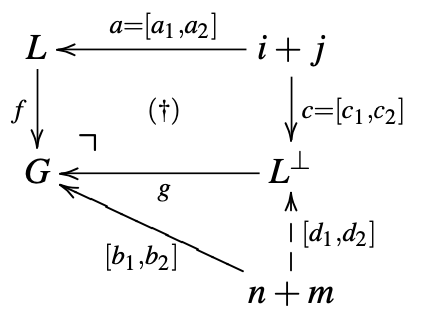
\includegraphics[width=0.3\linewidth]{figures/combinatorial_semantics/boundary_complement.png}
\end{figure}

is called a boundary complement if $[c_1, c_2]$ is mono and there exist $d_1 : n \to L^{\bot}$ and $d_2 : m \to L^{\bot}$ making the above triangle commute and such that
\[
    n + j \xrightarrow{[d_1,c_2]} L^{\bot} \xleftarrow{[d_2,c_1]} m + i
\]
is a monogamous cospan. 
\end{definition}

Intuitively, such a pushout complement requires that inputs get only glued to outputs and vice-verse in the two pushout squares.

\begin{definition}{Convex match}

We call a match $m : L \to G$ convex if it is mono and its image is a convex subgraph of $G$. 
    
\end{definition}

\begin{definition}{Rewriting in $\catname{MACsp_{D}({Hyp_{\Sigma}})}$}

Given $G \xleftarrow{} n+m$ and $H \xleftarrow{} n + m$ in $\catname{Hyp_{\Sigma}}$, $G$ rewrites convexly into $H$ with interface $n + m$ --- notation $(G \xleftarrow{} n + m ) \Rrightarrow_{\mathcal{R}}  (H \xleftarrow{} n + m )$ --- if there exist rule $L \xleftarrow{} i + j \xrightarrow{} R$ in $\mathcal{R}$ and object $C$ and cospan arrows $i+j \xrightarrow{} C \xleftarrow{} n+m$ in $\catname{Hyp_{\Sigma}}$ such that the DPOI diagram above commutes and its marked squares are pushouts and the following conditions hold

\begin{itemize}
    \item $m : L \to G$ is a convex match;
    \item $i + j \to C \to G$ is a boundary complement in the leftmost pushout.
\end{itemize}
    
\end{definition}

\textbf{Update: 4 Oct}

\begin{theorem}[Theorem 35~\cite{Frobenius2}]
\label{theorem:rewriting_no_frob}
    Let $R$ be any rewriting system on $\textsf{PROP}(\Sigma)$. Then,
    \[
    g \Rightarrow_{\mathcal{R}} h \;\text{ iff }\; \llangle ^{\ulcorner}g^{\urcorner} \rrangle \Rrightarrow_{\llangle \mathcal{R} \rrangle} \llangle ^{\ulcorner}h^{\urcorner} \rrangle 
    \]

    where $\llangle \cdot \rrangle : \textsf{PROP}(\Sigma) + Frob \to \catname{Csp_{D}(Hyp_{\Sigma})}$ is an isomorphism of props.
    \update{
        Last time I confused functors $\llangle \cdot \rrangle$ and $\llbracket \cdot \rrbracket$.
        Note that the result above is a weaker version of the same result for rewriting in $\textsf{PROP}(\Sigma) + Frob$.
        $Frob$ is an SMT with the signature $\Sigma_{Frob}$ which constitutes of \textit{only} Frobenius generators and terms are quotiented by both SMC laws and Frobenius equations.
        So, essentially, $Frob = \textsf{PROP}(\Sigma_{Frob}, \mathcal{E}_{Frob})$. 
        \question{Is it true that by quotienting $\textsf{PROP}(\Sigma)$ by SMC laws and quotienting $Frob$ by SMC and Frob laws we automatically quotient $\textsf{PROP}(\Sigma) + Frob$ by SMC and Frob laws?} 
    }
\end{theorem}

\begin{definition}[\;$\ulcorner \cdot \urcorner$]

    This is a syntactic operation which is defined for terms in $\textsf{PROP}(\Sigma) + Frob$ and is given below
    \[
        \tikzfig{combinatorial_semantics/bending_wires}
    \]
    
\end{definition}

\begin{remark}
    We need the operation above because we defined the rewriting for cospans of hypergraphs only for cospans of the form $0 \to G \xleftarrow{} n + m$ (for $\catname{Csp_{D}(Hyp_{\Sigma})},\; \MdaCospans,\; \MdaEcospans$), but the functors take arbitrary terms (string diagrams) as input.
    This operation turns an arbitrary term into a term with no inputs.
    Now the left-hand and right-hand sides are equivalent in the sense that $f \Rightarrow_{\langle l, r \rangle} g$ if and only if $\ulcorner f \urcorner \Rrightarrow_{\langle \ulcorner l \urcorner, \ulcorner r \urcorner \rangle} 
 \ulcorner g \urcorner$ and the latter string diagram can be interpreted as $0 \xrightarrow{} G \xleftarrow{} n + m$ for which we defined rewriting above.

\end{remark}

% \begin{proposition}
%     $m \xrightarrow{} \mathcal{G} \xleftarrow{} n$ is mda-cospan in $\MdaCospans$ iff $0 \xrightarrow{} \mathcal{G} \xleftarrow{} n + m$ is an mda-cospan.
% \end{proposition}

% In particular, the above proposition means that by fullness of $\llbracket \cdot \rrbracket$ there exists a corresponding SMC morphism for some $0 \xrightarrow{} \mathcal{G}\xleftarrow{} n + m$.
Theorem above essentially makes two routes below. In forward direction:

\[
\textsf{PROP}(\Sigma) \xrightarrow{i_1} \textsf{PROP}(\Sigma) + Frob \xrightarrow{\ulcorner \cdot \urcorner} \textsf{PROP}(\Sigma) + Frob \xrightarrow{\llangle \cdot \rrangle} \catname{Csp_{D}(Hyp_{\Sigma})}
\]

The proof of the theorem above in the forward direction then relies on the proof for rewriting in $\textsf{PROP}(\Sigma) + Frob$ and functoriality of $\llangle \cdot \rrangle$ and checking that a match is convex.

In backwards direction

\[
  \catname{Csp_{D}(Hyp_{\Sigma})} \xrightarrow{\llbracket \cdot \rrbracket}^{-1} \textsf{PROP}(\Sigma)  
\]

relies on decomposition of a hypergraph given a convex match and on fullness of 

\[
    \llbracket \cdot \rrbracket : \textsf{PROP}(\Sigma) \to \MdaCospans
\]

\question{What options we have?
\begin{enumerate}
    \item Define $PROP(\Sigma)^{+}$ and $PROP(\Sigma)^{+} + Frob$
    \item Say that $n \xrightarrow{} \mathcal{G} \xleftarrow{} m$ rewrites into $n \xrightarrow{} \mathcal{F} \xleftarrow{} m$ iff $0 \xrightarrow{} \mathcal{G} \xrightarrow{} n + m$ rewrites into $0 \xrightarrow{} \mathcal{F} \xrightarrow{} n + m$.
          This gives the following route
          \[
            \textsf{PROP}(\Sigma)^{+} \xrightarrow{\llbracket \cdot \rrbracket} \MdaEcospans \xrightarrow{\ulcorner \cdot \urcorner} \MdaEcospans
          \]

          and the same in the other direction with flipped arrows.
\end{enumerate}
}
\Aleksei{TODO: discuss this}

If we quotient $\MdaCospans$ by $\llangle \mathcal{R} \rrangle$ by the theorem~\ref{theorem:rewriting_no_frob} and faithfulness and fullness of $\llbracket \cdot \rrbracket$ we get the following result.
$f = g$ in $\textsf{PROP}(\Sigma,\mathcal{E})$ iff $\llangle ^{\ulcorner} f ^{\urcorner} \rrangle = \llangle ^{\ulcorner} f ^{\urcorner} \rrangle$ in $\MdaCospans$.

\question{Do we want the same result for $\textsf{PROP}(\Sigma, \mathcal{E})^{+}$ and $\WellTypedMdaEcospans$?}

\textbf{End of update}

We have a more general notion of interface and hence we need to adjust DPOI rewriting a little bit.
The first issue is that whole interfaces are not preserved during rewriting, consider an example in Figure~\ref{fig:example_rewrite_ecospans} which corresponds to a rewrite rule of $\langle f, f+g \rangle$.

\begin{figure}[t]
    \centering
    \[
    \scalebox{0.6}{\tikzfig{combinatorial_semantics/f_to_f_plus_g_example}}
    \]
    \caption{Example rewrite rule in $\WellTypedMdaEcospans$}
    \label{fig:example_rewrite_ecospans}
\end{figure}

The input interface on the left-hand side of the rule is $\{1, 2\}$, while the input interface on the right-hand side of the rule is $\{1,2,5,6,7,8\}$.
Note that the outermost interfaces are preserved.

Another concern is when we delete the occurrence of the left-hand side of a rewrite rule from an e-hypergraph we also modify this e-hypergraph's interfaces.
Consider a hypothetical DPO square below in Figure~\ref{fig:interface_change_example} where long arrows denote matching between carriers of cospans.

The first row of the diagram shows the span for a rewrite rule of $\langle f + g, f \rangle$ which is like a projection rule.
Note once again the difference between the interfaces of the left-hand and right-hand sides of the rewrite rule.
The entry in the middle of the span depicts the outermost interfaces which are preserved.
The second row depicts the e-hypergraph to be rewritten on the left and the result of the rewrite on the right.
The result is obtained by first deleting the image of the left-hand side of the rewrite rule from the initial e-hypergraph (depicted in the middle) and then gluing the right-hand side of the rewrite rule into it. 
Note that the interfaces of the initial e-hypergraph and the residual e-hypergraph are different. 
Here, the outermost and the whole interfaces for the eventual e-hypergraph coincide, but if the nested-ness of the initial e-hypergraph was more intense the result could have inner interfaces as well as we would remove the interfaces of the inner edges when deleting the image of the left-hand side part of the rule from the initial e-hypergraph.


\update{$i,j$ are replaced}

To account for such changes in the interfaces we put some additional constraints on DPOI rewriting.
Consider a DPOI diagram with extra constraints below which encodes
 the notion that cospan 
 $n_{ext} \xrightarrow{} g_i \xrightarrow{} G \xleftarrow{} g_o \xleftarrow{} m_{ext}$
 rewrites into a cospan 
 $n_{ext} \xrightarrow{} h_i \xrightarrow{} H \xleftarrow{} h_o \xleftarrow{} m_{ext}$ via a rewrite rule $\langle l, r \rangle$,
 where
 $l := x_{ext} \xrightarrow{} l_i \xrightarrow{} L \xleftarrow{} l_o \xleftarrow{} y_{ext}$
 and
 $r := x_{ext} \xrightarrow{} r_i \xrightarrow{} L \xleftarrow{} r_o \xleftarrow{} y_{ext}$.
 Note there are arrows from $x_{ext} + y_{ext} \to l_i + l_o$ (respectively, $r_i + r_o$) from the corresponding cospans which are not shown in the diagram.
 Similarly for the arrows from $n_{ext} + m_{ext}$.

% \[\begin{tikzcd}
% 	&&&& {i + j} \\
% 	{l_i+l_o} && L &&&& R && {r_i+r_o} \\
% 	\\
% 	{g_i+g_o} && {G^{\urcorner}} && C && {^{\ulcorner}H} && {h_i+h_o} \\
% 	\\
% 	&&&& {n+m}
% 	\arrow[color={rgb,255:red,214;green,92;blue,92}, from=1-5, to=2-3]
% 	\arrow[color={rgb,255:red,214;green,92;blue,92}, from=1-5, to=2-7]
% 	\arrow["m", color={rgb,255:red,214;green,92;blue,92}, from=2-3, to=4-3]
% 	\arrow["{[i_c,j_c]}", color={rgb,255:red,214;green,92;blue,92}, from=1-5, to=4-5]
% 	\arrow[color={rgb,255:red,214;green,92;blue,92}, from=2-7, to=4-7]
% 	\arrow["{[n_c,m_c]}"', color={rgb,255:red,214;green,92;blue,92}, from=6-5, to=4-5]
% 	\arrow[color={rgb,255:red,214;green,92;blue,92}, from=4-5, to=4-7]
% 	\arrow[color={rgb,255:red,214;green,92;blue,92}, from=4-5, to=4-3]
% 	\arrow[color={rgb,255:red,214;green,92;blue,92}, from=6-5, to=4-3]
% 	\arrow[color={rgb,255:red,214;green,92;blue,92}, from=6-5, to=4-7]
% 	\arrow[from=2-1, to=2-3]
% 	\arrow["{[f_i,f_o]}", from=2-1, to=4-1]
% 	\arrow[from=4-1, to=4-3]
% 	\arrow[from=2-9, to=2-7]
% 	\arrow[from=4-9, to=4-7]
% 	\arrow["{[h_i,h_o]}"{description}, from=2-9, to=4-9]
% 	\arrow[from=6-5, to=4-9]
% 	\arrow[from=6-5, to=4-1]
% 	\arrow["{[i_l,j_l]}"{description}, from=1-5, to=2-1]
% 	\arrow["{[i_r,j_r]}"{description}, from=1-5, to=2-9]
% \end{tikzcd}\]


% https://q.uiver.app/#q=WzAsMTEsWzIsMCwiTCJdLFs0LDAsInhfe2V4dH0gKyB5X3tleHR9Il0sWzIsMiwiR157XFx1cmNvcm5lcn0iXSxbNCwyLCJDIl0sWzQsNCwibl97ZXh0fSttX3tleHR9Il0sWzAsMCwibF9pK2xfbyJdLFswLDIsImdfaStnX28iXSxbNiwwLCJSIl0sWzYsMiwiXntcXHVsY29ybmVyfUgiXSxbOCwyLCJoX2kraF9vIl0sWzgsMCwicl9pK3JfbyJdLFsxLDAsIiIsMCx7ImNvbG91ciI6WzAsNjAsNjBdfV0sWzAsMiwibSIsMCx7ImNvbG91ciI6WzAsNjAsNjBdfSxbMCw2MCw2MCwxXV0sWzEsMywiW2lfYyxqX2NdIiwwLHsiY29sb3VyIjpbMCw2MCw2MF19LFswLDYwLDYwLDFdXSxbNCwzLCJbbl9jLG1fY10iLDIseyJjb2xvdXIiOlswLDYwLDYwXX0sWzAsNjAsNjAsMV1dLFszLDIsIiIsMix7ImNvbG91ciI6WzAsNjAsNjBdfV0sWzQsMiwiIiwyLHsiY29sb3VyIjpbMCw2MCw2MF19XSxbNSwwXSxbNiwyXSxbNCw4LCIiLDAseyJjb2xvdXIiOlswLDYwLDYwXX1dLFszLDgsIiIsMCx7ImNvbG91ciI6WzAsNjAsNjBdfV0sWzcsOCwiIiwyLHsiY29sb3VyIjpbMCw2MCw2MF19XSxbMSw3LCIiLDIseyJjb2xvdXIiOlswLDYwLDYwXX1dLFsxMCw3XSxbOSw4XV0=
\[
 \scalebox{0.75}{
    \tikzfig{combinatorial_semantics/DPOI_square_coloured}
 }
\]

The parts of the original DPOI square is shown in blue.
The extra bits simply account for more complicated interfaces.
For example, the left-hand side $L$ of a rewrite rule
 $\langle L, R \rangle$ which originally was some cospan
 $i \xrightarrow{} L \xleftarrow{} j$ in $\MdaCospans$ 
 now is a cospan
 $x_{ext} \xrightarrow{} l_i \to L \xleftarrow{} l_o \xleftarrow{} y_{ext}$
from $\WellTypedMdaEcospans$ where $l_i, l_o$ are whole input and output interfaces respectively.
The top half of this diagram says that the outermost interfaces
 should coincide for $L$ and $R$.
The bottom half puts the same restrictions on $G$ and $H$.
For the pushout to exist we impose our assumptions~\ref{pushout:assumptions} on the correspoding arrow.


We also adjust the definition of a boundary complement a bit.

\begin{definition}[Boundary complement in $\WellTypedMdaEcospans$]
\label{def:boundary_new}

% https://q.uiver.app/#q=WzAsNyxbMiwwLCJMIl0sWzQsMCwieF97ZXh0fSArIHlfe2V4dH0iXSxbMiwyLCJHXntcXHVyY29ybmVyfSJdLFs0LDIsIkMiXSxbNCw0LCJuX3tleHR9K21fe2V4dH0iXSxbMCwwLCJsX2krbF9vIl0sWzAsMiwiZ19pK2dfbyJdLFsxLDAsIiIsMCx7ImNvbG91ciI6WzAsNjAsNjBdfV0sWzAsMiwibSIsMCx7ImNvbG91ciI6WzAsNjAsNjBdfSxbMCw2MCw2MCwxXV0sWzEsMywiW2lfYyxqX2NdIiwwLHsiY29sb3VyIjpbMCw2MCw2MF19LFswLDYwLDYwLDFdXSxbNCwzLCJbbl9jLG1fY10iLDIseyJjb2xvdXIiOlswLDYwLDYwXX0sWzAsNjAsNjAsMV1dLFszLDIsIiIsMix7ImNvbG91ciI6WzAsNjAsNjBdfV0sWzQsMiwiIiwyLHsiY29sb3VyIjpbMCw2MCw2MF19XSxbNSwwXSxbNiwyXV0=
\[
\scalebox{0.75}{
    \tikzfig{combinatorial_semantics/DPOI_pushout_complement}
}
\]

Consider the diagram above where the marked square is a pushout
 and $x_{ext} + y_{ext}$ and $n_{ext} + m_{ext}$ are 
 the \textit{outermost} interfaces for the corresponding 
 cospans.
We say that $x_{ext} + y_{ext} \to C \to G^{\urcorner}$ is 
 a \textit{boundary} complement if $[i_c, i_j]$ is mono 
 and there exist $n_c : n_{ext} \to C$ and $m_c : m_{ext} \to C$ 
 making the above triangle commute and such that
there exists a \textit{not necessarily well-typed} mda-cospan

\[
n_{ext} \xrightarrow{} c_i + y_{ext} \xrightarrow{} C \xleftarrow{} c_o + x_{ext} \xleftarrow{} m_{ext}
\]

where $c_i$ and $c_o$ are computed as
 $c_i = g_i \setminus (l_i \setminus x_{ext})$ and
 $c_o = g_o \setminus (l_o \setminus y_{ext})$.
\end{definition}

\begin{figure}
    \centering
    \[
    \scalebox{0.5}{\tikzfig{combinatorial_semantics/interfaces_change_example}}\]
    \caption{Hypothetical DPO square for $\catname{MACsp_{D}(EHyp_{\Sigma})}$}
    \label{fig:interface_change_example}
\end{figure}

% The second point above means that when cutting the mono-occurrence of $L$ out from $G$ we also need to remove the inner interfaces of $L$ from the whole interface of $G$. \question{According to the pushout squares above, $c_i$ is constructed by removing from $g_i$ everything from $l_i$ which does not have a pre-image in $i$, i.e., everything except the outermost interfaces (same holds for $c_o$)}

\begin{remark}
Note that cospan $n_{ext} \xrightarrow{} c_i + y_{ext} \xrightarrow{} C \xleftarrow{} c_o + x_{ext} \xleftarrow{} m_{ext}$ is not well-typed.
The cospan's input interface contains nodes that previously were a part of the output interface.
\end{remark}

First, let's check that this notion generalises the ordinary boundary complement from~\ref{def:boundary_original}.
For this, we assume that $<_{c}$ and $\consistency^{\mu}$ relations are empty in which case $x_{ext} + y_{ext}$ and $l_i + l_o$ coincide as well as $g_i + g_o$ and $n_{ext} + m_{ext}$.
Hence, $g_i \setminus (l_i \setminus x_{ext}) + y_{ext} = g_i + y_{ext} = n_{ext} + y_{ext}$ and the same for the output interfaces.
Thus we have $n_{ext} + y_{ext} \xrightarrow{} C \xleftarrow{} m_{ext} + x_{ext}$, which corresponds to the definition from~\ref{def:boundary_original}.

% Next, consider an example from figure~\ref{fig:dpoir}. The outermost interfaces of $L$ coincide with the whole interfaces, i.e. $l_i + l_o = i + j$. However, $n + m = \{0'', 1''\}$ and $g_i + g_o = \{0'',0,2,1,3,1''\}$. According to the definition of a boundary complement the following mda cospan should exist: $g_i \setminus (l_i \setminus i) + j = \{0'', 0, 2\} \setminus \varnothing \cup \{1\} = \{0'',0,2,1\} \xrightarrow{} C \xleftarrow{} \{0,1,3,1''\} = \text{same procedure for output interfaces}$.

% \question{We need to show that this boundary complement is unique and that after performing a pushout on the right the result is also an mda hypergraph}

% We can now present a complete DPOI square

% \[
% \begin{tikzcd}
%                    &                    & i+j \arrow[ld] \arrow[lld] \arrow[ddd, "f"] \arrow[rrd] \arrow[rd] &                    &              &  &                       &               &                       &               \\
% L \arrow[dd, "m"'] & l_i+l_o \arrow[l]  &                                                                    & r_i+r_j \arrow[r]  & R \arrow[dd] &  & i \arrow[r] \arrow[d] & r_i \arrow[d] & j \arrow[d] \arrow[r] & r_o \arrow[d] \\
%                    &                    &                                                                    &                    &              &  & c_i \arrow[r]         & h_i           & c_o \arrow[r]         & h_o           \\
% G                  &                    & C \arrow[ll] \arrow[rr]                                            &                    & H            &  &                       &               &                       &               \\
%                    & g_i+g_o \arrow[lu] & n+m \arrow[u] \arrow[l] \arrow[llu] \arrow[r] \arrow[rru]          & h_i+h_o \arrow[ru] &              &  &                       &               &                       &              
% \end{tikzcd}
% \]



% \begin{remark}
%     Note that in all pushout squares for the interfaces all the morphisms are monos. \question{Does it follow from anything above? Because the corresponding triangles commute?}
% \end{remark}



\begin{proposition}
    The boundary complement in~\ref{def:boundary_new} when exists is unique
    \begin{proof}
        \update{I will try to reinvent a similar proof from~\cite{Frobenius2} as the cited proof does not make sense to me}
        The pushout in $EHyp_{\Sigma}$ should also be a pushout on the underlying sets of nodes and hyperedges.
        Hence, pushout complement should yield pushout complements for the sets of nodes and hyperedges.
        In particular,
          % https://q.uiver.app/#q=WzAsNSxbMCwwLCJWX3tMfSJdLFsyLDAsImxfe2l9ICsgbF97b30iXSxbNCwwLCJpK2oiXSxbMCwyLCJWX3tHfSJdLFs0LDIsIlZfe0N9Il0sWzIsMSwiYl97Vn0iXSxbMSwwLCJhX3tWfSJdLFswLDMsImZfe1Z9Il0sWzQsMywiZ197Vn0iLDJdLFsyLDQsImMiLDJdXQ==
    \begin{figure}[h!]
        \begin{subfigure}{0.45\textwidth}
            \[\begin{tikzcd}
                {V_{L}} && {l_{i} + l_{o}} && {i+j} \\
                \\
                {V_{G}^{\urcorner}} &&&& {V_{C}}
                \arrow["{b_{V}}", from=1-5, to=1-3]
                \arrow["{a_{V}}", from=1-3, to=1-1]
                \arrow["{f_{V}}", from=1-1, to=3-1]
                \arrow["{g_{V}}"', from=3-5, to=3-1]
                \arrow["c"', from=1-5, to=3-5]
            \end{tikzcd}\]
        \end{subfigure}
        \hfill
        \begin{subfigure}{0.45\textwidth}
           % https://q.uiver.app/#q=WzAsNSxbMCwwLCJFX3tMfSJdLFsyLDAsIjAiXSxbNCwwLCIwIl0sWzAsMiwiRV97R31ee1xcdXJjb3JuZXJ9Il0sWzQsMiwiRV97Q30iXSxbMiwxLCJiX3tFfSJdLFsxLDAsImFfe0V9Il0sWzAsMywiZl97RX0iXSxbNCwzLCJnX3tFfSIsMl0sWzIsNCwiYyIsMl1d
        \[
        \begin{tikzcd}
            {E_{L}} && 0 && 0 \\
            \\
            {E_{G}^{\urcorner}} &&&& {E_{C}}
            \arrow["{b_{E}}", from=1-5, to=1-3]
            \arrow["{a_{E}}", from=1-3, to=1-1]
            \arrow["{f_{E}}", from=1-1, to=3-1]
            \arrow["{g_{E}}"', from=3-5, to=3-1]
            \arrow["c"', from=1-5, to=3-5]
        \end{tikzcd}
        \]
        \end{subfigure}
    \end{figure}
    $V$s and $E$s are sets of nodes and hyperedges respectively, marked squares are pushouts and $C$s are pushout complements.
    Because $i+j$ is discrete, $E_{G}^{\urcorner}$ is the disjoint union of $E_{L}$ and $E_{C}$ and hence $E_{C} = E_{G}^{\urcorner} \setminus E_{L}$.
    Then, since all the arrows are monos, the left square can be rewritten as follows.
    \[
      % https://q.uiver.app/#q=WzAsNSxbMCwwLCJpICsgaiArIHggKyB5Il0sWzIsMCwiaStqICsgeCJdLFs0LDAsImkraiJdLFswLDIsImkgKyBqICsgeCArIHkgKyB6Il0sWzQsMiwiaSArIGogKyB3IFxcY29uZyBpICsgaiArIHoiXSxbMiwxLCJiX3tWfSJdLFsxLDAsImFfe1Z9Il0sWzAsMywiZl97Vn0iXSxbNCwzLCJnX3tFfSIsMl0sWzIsNCwiYyIsMl1d
    \begin{tikzcd}
        {i + j + x + y} && {i+j + x} && {i+j} \\
        \\
        {i + j + x + y + z} &&&& {i + j + w \cong i + j + z}
        \arrow["{b_{V}}", from=1-5, to=1-3]
        \arrow["{a_{V}}", from=1-3, to=1-1]
        \arrow["{f_{V}}", from=1-1, to=3-1]
        \arrow["{g_{E}}"', from=3-5, to=3-1]
        \arrow["c"', from=1-5, to=3-5]
    \end{tikzcd}
    \]
    Because $i + j + x + y + w$ also yields a pushout it must be the case that $i+j+x+y+w \cong i + j + x + y + z$ and therefore $w \cong z$ and pushout complement for nodes is $i + j + z$ up to isomorphism.
    To show that pushout complement is unique we next need to show that source and target maps are unique.
    Suppose that there exist
    \[
        C_{1} = (V_{C}, V_{E}, s_{1},t)
    \]
    and
    \[
        C_{2} = (V_{C},V_{E},s_{2},t)
    \]
    Because $g$ is a homomorphism, it must be the case that $g_{V}^{*}(s_{1}(h)) = s_{G}^{*}(g_{E}(h)) = g_{V}^{*}(s_{2}(h))$.
    Because $g$ is mono, $g_{V}^{*}(s_{1}(h)) = g_{V}^{*}(s_{2}(h))$ implies $s_{1}(h) = s_{2}(h)$.
    Similarly for targets.
    We also need to show that $<_{c}$ and $\consistency^{\mu}$ are unique.
    Suppose that there exist
    \[
        C_{1} = (V_{C}, V_{E}, s,t, <_{1})
    \]
    and
    \[
        C_{2} = (V_{C},V_{E},s,t, <_{2})
    \]
    Because $g$ is homomorphism, it must be the case that $g_{E}(<_{1}(i_{V_{C}}(v))) = <_{G}(i_{V_{G}}(g_{V}(v))) = g_{E}(<_{2}(i_{V_{C}}(v)))$ which implies $<_{2}(i_{V_{C}}(v)) = <_{1}(i_{V_{C}}(v))$ for all $v$ such that $[v) \not = \varnothing$.
    Similarly for edges.
    Now suppose that $<_{1}(i_{V_{C}}(v)) = e$ and $<_{2}(i_{V_{C}}(v))$ is undefined.
    Then, $g_{E}(e) = <_{G}(i_{V_{G}}(g_{V}(v)))$ and there exists $v' \in V_{L}$ and $v'' \in V_{C_{2}}$ such that $[v') \not = \varnothing$ and there is a path from $v$ to $v''$ and $v''$ and $v'$ share a pre-image in $i+j$.
    However, because there is a path from $v$ to $v''$ it must be the case that $[v'') \not = \varnothing$ in $C_{1}$, but then it violates our assumptions as there exists some node $u$ in $i+j$ such that $v'' = c_{V}(u)$ and $[v'') \not = \varnothing$ and $v' = b_{V};a_{V}(u)$ and $[v') \not = \varnothing$.
    Therefore we get a contradiction. 
    Similarly for edges.
    Finally, let's suppose there exist
    \[
        C_{1} = (V_{C}, V_{E}, s,t, <, \consistency_{1}^{\mu})
    \]
    and
    \[
        C_{2} = (V_{C},V_{E},s,t,<, \consistency_{2}^{\mu})
    \]
    Because $g$ is a homomorphism, we have
    \[
        \langle g_{V};i_{V_{G}}, g_{E};i_{E_{G}} \rangle^{*}(\consistency_{C_1}^{\mu}(i_{V_{C}}(v))) \subseteq \consistency_{G}^{\mu}(g_{V};i_{V_{G}}(v))
    \]
    \[
        \langle g_{V};i_{V_{G}}, g_{E};i_{E_{G}} \rangle^{*}(\consistency_{C_2}^{\mu}(i_{V_{C}}(v))) \subseteq \consistency_{G}^{\mu}(g_{V};i_{V_{G}}(v))  
    \]
    \begin{itemize}
        \item If $\consistency_{G}^{\mu}(g_{V};i_{V_{G}}(v)) = \varnothing$ then both lefthand sides should be $\varnothing$ and the relations are equal.
        \item Suppose that $\consistency_{G}^{\mu}(g_{V};i_{V_{G}}(v)) \not = \varnothing$ which further means that $[g_{V};i_{V_{G}}(v)) \not = \varnothing$.
        \begin{itemize}
            \item $\consistency_{C_1}^{\mu}(i_{V_{C}}(v)) \subseteq \consistency_{C_2}^{\mu}(i_{V_{C}}(v))$.
                  This means that there exists $v'$ such that $v' \consistency_{C_{2}}^{\mu} v$ and $v' \not \consistency_{C_{1}}^{\mu} v$.
                  Because $g_{V}(v) \consistency^{\mu} v'$ it means that there exists $u,u'$ such that there is a path from $v$ to $u$ and from $v'$ to $u'$ and there exist $w,w' \in V_{L}$ such that $w \consistency_{L}^{\mu} w'$ and $w,u$ share pre-image in $i+j$ as well as $w',u'$.
                  This again contradicts our assumptions as $u \consistency_{C_{2}}^{\mu} u'$ and $w \consistency_{L}^{\mu} w'$.
            \item $\consistency_{C_1}^{\mu}(i_{V_{C}}(v)) \cap \consistency_{C_2}^{\mu}(i_{V_{C}}(v)) = \varnothing$
                  Similar to the above.
            \item $\consistency_{C_1}^{\mu}(i_{V_{C}}(v)) \cap \consistency_{C_2}^{\mu}(i_{V_{C}}(v)) \not = \varnothing$
                  Similar to the above.
        \end{itemize}
    \end{itemize}
    \end{proof}
    \update{Can we check the proof? I haven't used all the conditions from monogamous-ness above.
    Although, if the morphism $i+j \to L$ is mono, the complement is unique for not-monogamous hypergraphs as well.}
\end{proposition}


\question{
\begin{definition}[Convex down-closed match] 
    We call $m : L \to G$ in $\catname{EHyp_{\Sigma}}$ a convex down-closed match if
    
    \begin{enumerate}
        \item $m$ is monomorphism
        \item $m(L)$ is a convex down-closed subgraph of $G$
        \item \update{I've removed the requirement that consistency should be reflected because well typedness prohibits otherwise formed matches.}
    \end{enumerate}
\end{definition}
}


\begin{definition}[Rewriting in $\WellTypedMdaEcospans$]
    Given $G \xleftarrow{} g_i + g_o \xleftarrow{} n_{ext} + m_{ext}$ 
    and $H \xleftarrow{} h_i + h_o \xleftarrow{} n_{ext} + m_{ext}$ in $\Ecospans$ with the outermost interfaces $n_{ext} + m_{ext}$, $G$ rewrites convexly into $H$ with the outermost interface $n_{ext} + m_{ext}$ --- notation $( G \xleftarrow{} n_{ext} + m_{ext} ) \Rrightarrow_{\mathcal{R}} (E \xleftarrow{} n_{ext} + m_{ext} )$ --- if there exists a rule $l_i + l_o \xrightarrow{} L \xleftarrow{} x_{ext} + y_{ext} \xrightarrow{} R \xleftarrow{} r_i + r_o$ with the outermost interfaces $x_{ext} + y_{ext}$ in $\mathcal{R}$ and object $C$ and cospan arrows $x_{ext} + y_{ext} \xrightarrow{} C \xleftarrow{} n_{ext} + m_{ext}$ in $\Ecospans$ such that the diagram below commutes and its marked squares are pushouts

% https://q.uiver.app/#q=WzAsMTEsWzIsMCwiTCJdLFs0LDAsInhfe2V4dH0gKyB5X3tleHR9Il0sWzIsMiwiR157XFx1cmNvcm5lcn0iXSxbNCwyLCJDIl0sWzQsNCwibl97ZXh0fSttX3tleHR9Il0sWzAsMCwibF9pK2xfbyJdLFswLDIsImdfaStnX28iXSxbNiwwLCJSIl0sWzYsMiwiXntcXHVsY29ybmVyfUgiXSxbOCwyLCJoX2kraF9vIl0sWzgsMCwicl9pK3JfbyJdLFsxLDAsIiIsMCx7ImNvbG91ciI6WzAsNjAsNjBdfV0sWzAsMiwibSIsMCx7ImNvbG91ciI6WzAsNjAsNjBdfSxbMCw2MCw2MCwxXV0sWzEsMywiW2lfYyxqX2NdIiwwLHsiY29sb3VyIjpbMCw2MCw2MF19LFswLDYwLDYwLDFdXSxbNCwzLCJbbl9jLG1fY10iLDIseyJjb2xvdXIiOlswLDYwLDYwXX0sWzAsNjAsNjAsMV1dLFszLDIsIiIsMix7ImNvbG91ciI6WzAsNjAsNjBdfV0sWzQsMiwiIiwyLHsiY29sb3VyIjpbMCw2MCw2MF19XSxbNSwwXSxbNiwyXSxbNCw4LCIiLDAseyJjb2xvdXIiOlswLDYwLDYwXX1dLFszLDgsIiIsMCx7ImNvbG91ciI6WzAsNjAsNjBdfV0sWzcsOCwiIiwyLHsiY29sb3VyIjpbMCw2MCw2MF19XSxbMSw3LCIiLDIseyJjb2xvdXIiOlswLDYwLDYwXX1dLFsxMCw3XSxbOSw4XV0=
\[\scalebox{0.75}{
    \tikzfig{combinatorial_semantics/DPOI_square}
    }
\]
    and the following conditions hold

    \begin{enumerate}
        \item $m : L \to G$ is a convex down-closed match;
        \item $x_{ext} + y_{ext} \to C \to G$ is a boundary complement in the leftmost pushout.
    \end{enumerate}
\end{definition}


\Aleksei{Do we need to introduce substitution? This is needed if our rewrite rules are going to have variables as labels.}


The whole interfaces of the resulting e-hypergraph $H$ from the cospan
 $n_{ext} \xrightarrow{} h_i \xrightarrow{} H \xleftarrow{} h_o \xleftarrow{} m_{ext}$
 are constructed as $h_i = (r_i \setminus x_{ext}) + c_i$ 
 and
 $h_o = (r_o \setminus y_{ext}) + c_o$.
 $h_i \to H$ is defined as a copairing of 
 $f_1 : r_i \setminus x_{ext} \to R \to H$ 
 and 
 $f_2 : c_i \to C \to H$. 
Since both $f_1$ and $f_2$ are mono, their copairing is also a mono. 
Similarly for $h_o$.

We then say that an mda-cospan 
\[
    n_{ext} \xrightarrow{a_1} g_{i} \xrightarrow{a_2} G \xleftarrow{b_2} g_{o} \xleftarrow{b_1} m_{ext}
\]
rewrites convexly into another mda-cospan

\[
    n_{ext} \xrightarrow{a_1} h_{i} \xrightarrow{a_2} H \xleftarrow{b_2} h_{o} \xleftarrow{b_1} m_{ext}
\]

under a rewrite rule 
\[
    \langle x_{ext} \xrightarrow{a_1} l_{i} \xrightarrow{a_2} L \xleftarrow{b_2} l_{o} \xleftarrow{b_1} y_{ext}, 
    x_{ext} \xrightarrow{a_1} r_{i} \xrightarrow{a_2} R \xleftarrow{b_2} r_{o} \xleftarrow{b_1} y_{ext} \rangle
\]

if 
\[
    G \xleftarrow{\langle a_2,b_2 \rangle} g_i + g_{o} \xleftarrow{\langle a_1, b_1 \rangle} n_{ext} + m_{ext} \Rrightarrow H \xleftarrow{\langle a_2,b_2 \rangle} h_i + h_{o} \xleftarrow{\langle a_1, b_1 \rangle} n_{ext} + m_{ext}
\]
under a rewrite rule
\[
    \langle l_{i} + l_{o} \xrightarrow{\langle a_2, b_2 \rangle} L \xleftarrow{\langle a_1, b_1 \rangle} x_{ext} + y_{ext},
    r_{i} + r_{o} \xrightarrow{\langle a_2, b_2 \rangle} R \xleftarrow{\langle a_1, b_1 \rangle} x_{ext} + y_{ext} 
    \rangle
\]

\begin{proposition}

$n_{ext} \xrightarrow{n_h} h_i \xrightarrow{f} H \xleftarrow{g} h_o \xleftarrow{m_h} m_{ext}$ is a well-typed mda-cospan.

\begin{proof}
$f$ and $g$ are monos by construction.
$n_{ext} + m_{ext} \to h_i + h_o$ is a mono by commutativity because $n_{ext} + m_{ext} \to H$ is a mono (also by commutativity). 
The only in-degree 0 nodes have a pre-image in $c_i$ and $r_i \setminus x_{ext}$  and end up being in the image of $h_i$ (the nodes with the pre-image in $y_{ext}$ get glued together).
Well-typedness is restored once the right-hand side of the rewrite rule is glued into $C$.
\end{proof}
\end{proposition}

\Aleksei{Check the proof}

\Aleksei{Can we reuse anything from~\cite{Frobenius}?}

Consider an example below that illustrates the introduced constraints.

\update{I've switched to $[ \cdot ]$ for our functor to be able to differenciate between $\llbracket \cdot \rrbracket$, $\llangle \cdot \rrangle$}
\begin{remark}
    For now, we will informally denote a combinatorial interpretation of a morphism $f$ in $\textsf{PROP}^{+}(\Sigma)$ as $[ f ]$.
\end{remark}

\begin{example}

A DPOI square for rewriting in $\WellTypedMdaEcospans$ is depicted in Figure~\ref{fig:refined_dpoi}.
A projection rule of $\llbracket f + g \rrbracket \to \llbracket f \rrbracket$ is shown in the top half of the diagram.
The image of the matching $m$ is shown in red and its image is a convex down-closed e-hypergraph.
Pushout complement is then computed by removing the image of $m$ from the target e-hypergraph by keeping intact the nodes that have a pre-image in the carrier of the rewriting span. The corresponding mda-cospan is depicted at the bottom: $c_i = g_i \setminus (l_i \setminus i) = \{18, 19, 1, 2, 13, 14, 5, 6, 7, 8\} \setminus (\{1,2,5,6,7,8\} \setminus \{1,2\}) = \{18, 19, 1, 2, 13, 14, 5, 6, 7, 8\} \setminus \{5,6,7,8\} = \{18,19,1,2,13,14\}$ and $c_i + j = \{18,19, 1, 2, 13, 14, 3, 4\}$ which is the input interface for $C$. Similar computations are performed for $c_o$. Then pushout glues $R$ and $C$ together along $i + j$ and the resulting interface $h_i = c_i + (r_i \setminus i) = \{18,19, 1, 2, 13, 14\} + \varnothing = \{18,19, 1, 2, 13, 14\}$ and likewise for $h_o$.

%     \begin{figure}
%         \centering
% \[
%   \scalebox{0.3}{      \tikzfig{combinatorial_semantics/refined_dpoi_example}
% }
%         \]
%     \caption{Refined DPOI rewriting}
%     \label{fig:refined_dpoi}
%     \end{figure}
    
\end{example}

\Aleksei{This figure yeilds "Dimension too large". Need to fix it.}

Unlike SMC equations the equations for semilattice enriched categories are not absorbed by e-hypergraph representation and hence to further build a correspondence between $\textsf{PROP}^{+}(\Sigma)$ and $\WellTypedMdaEcospans$ we add them as structural rewrite rules.
Recall that the category $\catname{EHyp_{\Sigma}}$ does not have all pushouts and hence we need to explicitly show that the pushouts that we need exist.


\begin{proposition}
Pushouts for all semilattice enrichment equations exist.

\begin{proof}
    Let us give a combinatorial interpretation for an instance of the first equation (distributivity) in~\ref{fig:string-equations}.
    It can be found in Figure~\ref{fig:distributivity_interpretation}.
    After we identify a convex down-closed image of the left-hand side of this rule within a graph $G$ we remove the image by keeping only the outermost nodes.
    Note that because the image of all $a$'s and $b$'s are outermost nodes, we are allowed to pick any monomorphism for our pushout complement.
    And for the same reason the pushout for the right square exists.
    Then we simply glue the right-hand side of the rule into the hole.
    Such equations are not absorbed by e-hypergraph representation unlike SMC equations because the right-hand side contains more edges, i.e. graphs $G$ and $H$ are not isomorphic.
    Similar argument applies to other rules as well.
\end{proof}
\end{proposition}

\update{I think I haven't paid any attention to this fact previously, but it seems that in~\cite{Frobenius} the functor $\llbracket - \rrbracket$ is between $PROP_{\Sigma_{Frob}}$ and $Csp_{D}(Hyp_{\Sigma})$, i.e. PROP is quotiented by Frobenius equations, but they are absorbed in hypergraphs domain. We will have a similar thing: $\llbracket - \rrbracket: PROP^{+}_{\Sigma^{+}} \to \WellTypedMdaEcospans_{R^+}$, i.e. we will quotient PROP$^{+}$ by semilattice equations and quotient e-hypergraphs by the interpretation of these equations as they are not absorbed. The quotienting on the left is always implicit?}

\begin{figure}
    \centering
    \[
    \scalebox{0.45}{
    \tikzfig{combinatorial_semantics/structural_rule_pushout}}\]  
    \caption{Distributivity rewrite rule interpretation}
    \label{fig:distributivity_interpretation}
\end{figure}

\begin{definition}
    We will denote with $\mathcal{S}$ the interpretation of the equations in~\ref{fig:string-equations} as rewrite rules in $\WellTypedMdaEcospans$.
    In particular, for all $l = r$ in~\ref{fig:string-equations}, $\mathcal{S}$ will contain $\langle [l], [r]\rangle$ and $\langle [r], [l] \rangle$.
    \update{Technically we add those for all possible instances of $l$ and $r$ in~\ref{fig:string-equations}.}
\end{definition}


\begin{remark}
    There is a minor limitation for DPOI rewriting above. It is unable to express rewriting for rules that contain an edge with no inputs and outputs on their right-hand side. This is because there is no way to impose both conflict and child relation of such an edge as it has no incident nodes in its context. An example of this could be seen in Figure~\ref{fig:non_expressible}. After an image of a match is removed there is no way of plugging $k$ into the hierarchical edge as it has no connection with this edge via the shared interface. However, we think that this is only a minor limitation because in practice such edges with no incident nodes correspond to `scalars' if we consider for example a category of vector spaces where a rewrite rule with a scalar could be

\begin{alignat*}{3}
\begin{pmatrix}
 1 &  2 \\
-1 &  1 \\
\end{pmatrix}
&\!\begin{aligned}
\hspace{1em} & \otimes &
\end{aligned}
&\!\begin{aligned}
2 &
\end{aligned}
&\!\begin{aligned}
 & \xrightarrow{} & 
\end{aligned}
&\!\begin{aligned}
\begin{pmatrix}
 2 &  4 \\
-2 &  2 \\
\end{pmatrix}    
\end{aligned}
\end{alignat*}
\end{remark}

That is, typically such scalars are absorbed and not present on the right-hand side of a rewrite rule.

\begin{figure}
    \centering
\[
\scalebox{0.5}{
\tikzfig{combinatorial_semantics/non_expressible_rewrite}
}
\]
    \caption{Non expressible rewrite}
    \label{fig:non_expressible}
\end{figure}

\newpage